\documentclass[preprint,12pt]{elsarticle}

\usepackage{float}
\usepackage{amssymb}
\usepackage{amsmath}
\usepackage{booktabs} 
\usepackage{adjustbox}
\usepackage{textcomp}
\usepackage{comment}
\usepackage{lineno}
\usepackage[colorlinks=true, linkcolor=blue, citecolor=blue, urlcolor=blue]{hyperref}
\usepackage{url}
\usepackage{pifont}
\usepackage{makecell}
\usepackage{hyphenat}
\usepackage[T1]{fontenc}

\hypersetup{
  pdftitle={Developing a prototype decision support framework to assess forest management scenarios as a nature-based decarbonization solution for the mining sector: A case study in British Columbia, Canada},
  pdfauthor={Elaheh Ghasemi, Kathleen Coupland, Salar Ghotb, Gregory Paradis},
  pdfsubject={Submitted to Sustainable Futures},
  pdfkeywords={decision support, forest management, nature-based solutions, mining, carbon accounting, prototype}
}

\journal{Cleaner Environmental Systems}
\biboptions{sort&compress}

\begin{document}

% Graphical abstract (for submission; image also uploaded separately)
\begin{graphicalabstract}
\centering
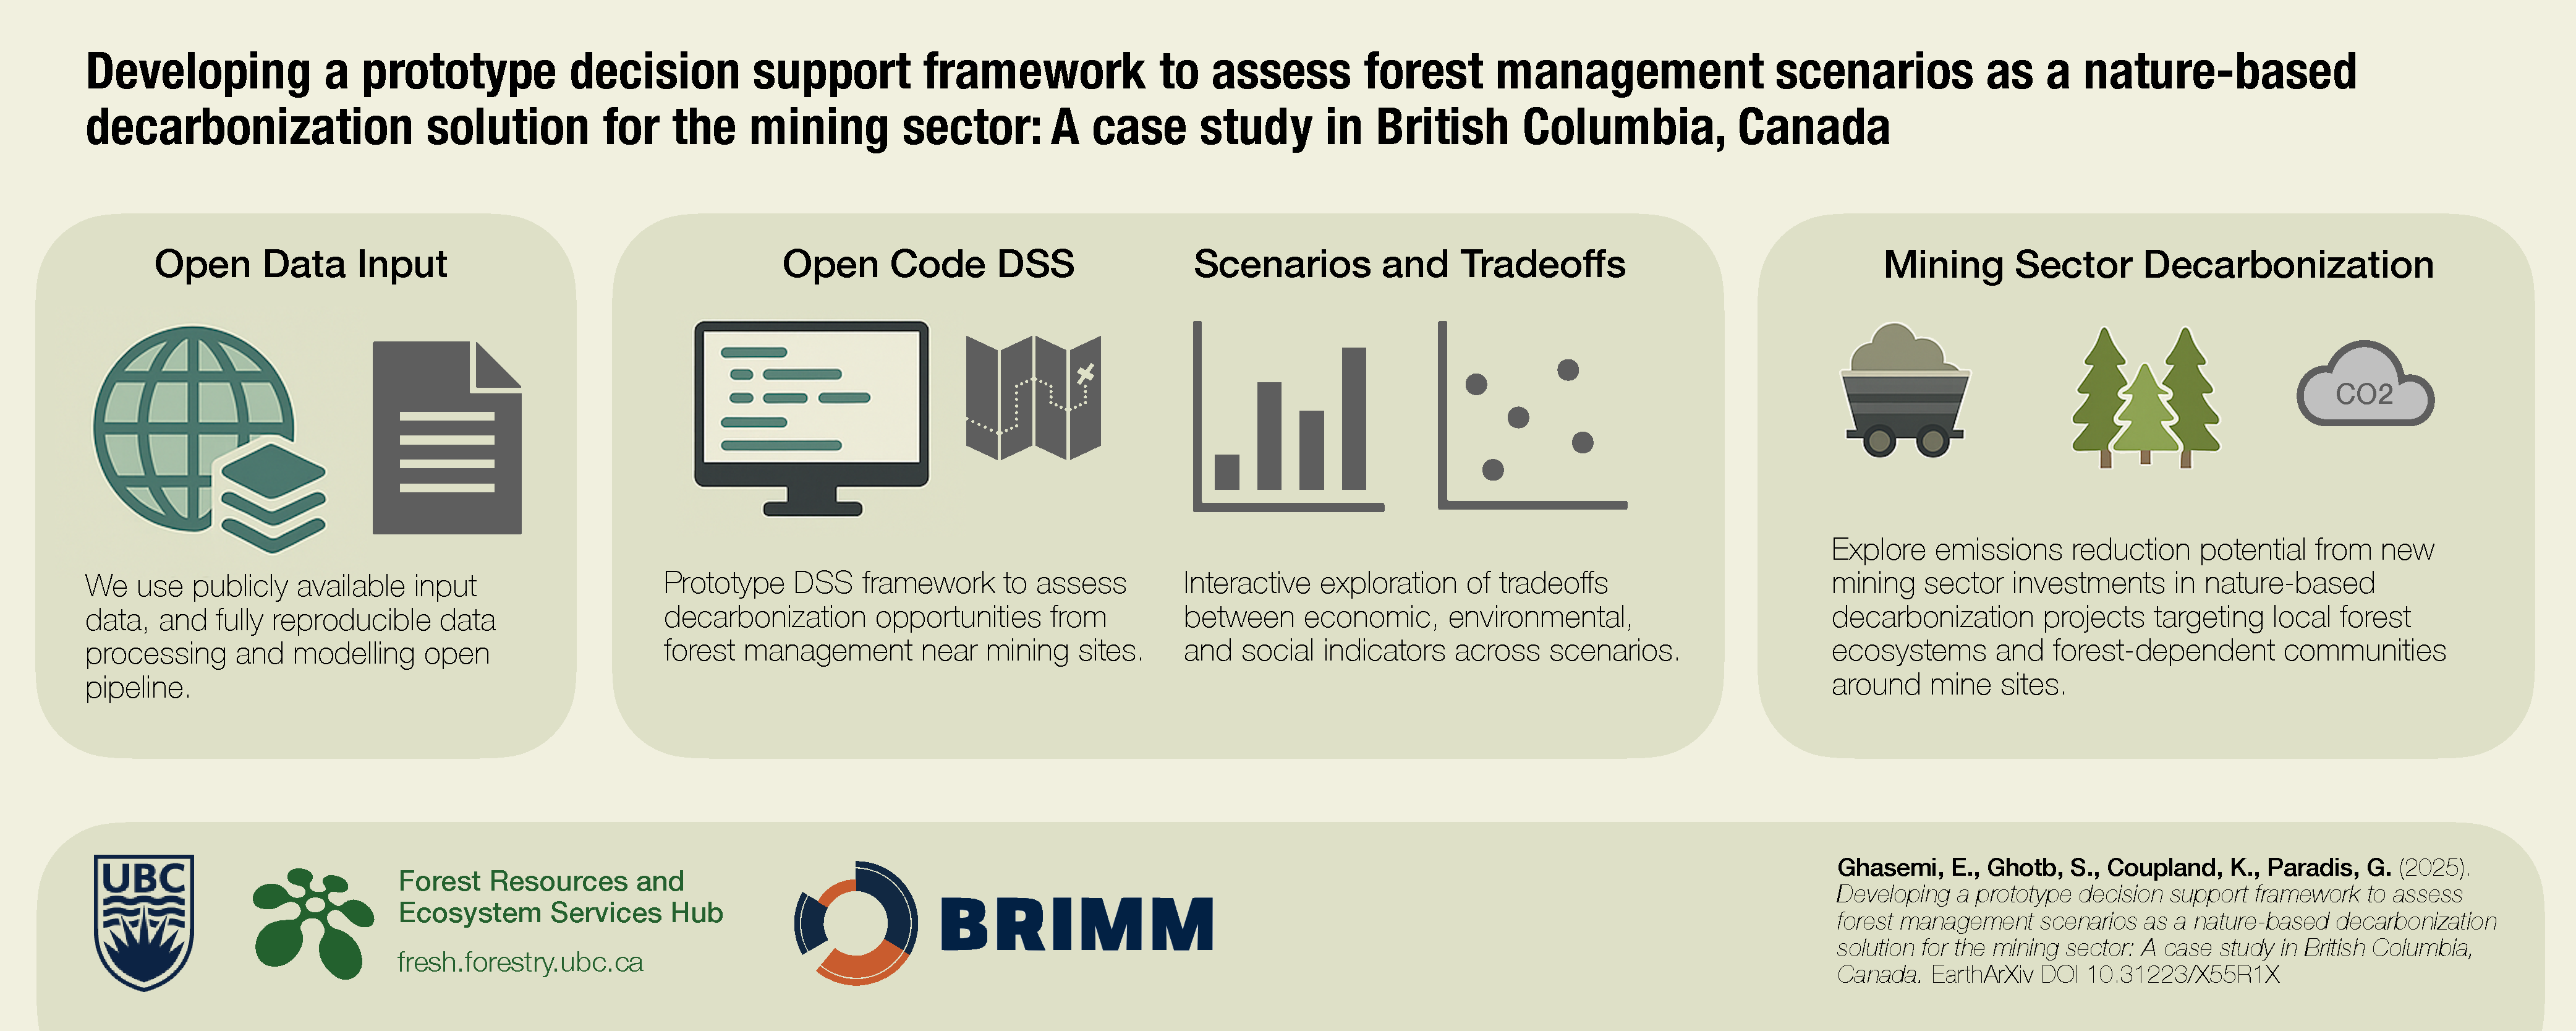
\includegraphics[width=\textwidth]{nbds_dss_manuscript_graphical-abstract.pdf}
\end{graphicalabstract}

% Research highlights (3–5 concise bullet points)
\begin{highlights}
\item Develops a prototype decision support framework for forest management near mining sites
\item Integrates publicly available geospatial and inventory data to estimate harvest and carbon outcomes
\item Evaluates alternative objectives: maximizing harvested volume, minimizing harvested area, maximizing ecosystem carbon stocks, and minimizing net emissions
\item  Quantifies trade-offs among environmental and economic indicators
\item Informs decarbonization planning by assessing forest-based emissions mitigation pathways
\end{highlights}
\begin{frontmatter}

\title{Developing a prototype decision support framework to assess forest management scenarios as a nature-based decarbonization solution for the mining sector: A case study in British Columbia, Canada}

\author[1]{Elaheh Ghasemi}
\ead{elaheh.ghasemi@ubc.ca}
\author[1]{Kathleen Coupland}
\ead{kathleen.coupland@ubc.ca}
\author[1]{Salar Ghotb}
\ead{salar.ghotb@ubc.ca}
\author[1]{Gregory Paradis\corref{cor1}}
\ead{gregory.paradis@ubc.ca}

\address[1]{Faculty of Forestry, University of British Columbia, 2424 Main Mall, Vancouver, BC V6T 1Z4, Canada}

\cortext[cor1]{Corresponding author.}

\begin{abstract}
This study, conducted with a leading gold producer, investigates how forest management nature-based solutions can support pathways to carbon neutrality by 2050. We present a prototype open-source decision support framework that assembles publicly available geospatial, inventory, and landscape modeling data to evaluate forest management scenarios around three British Columbia mining sites.

The framework compares business-as-usual harvesting with alternatives optimized to maximize harvested volume, minimize harvested area, maximize ecosystem carbon stocks, or minimize net emissions. It tracks environmental indicators and quantifies the trade-off between foregone harvest revenues and emission reductions, demonstrating how forest management around mining sites can offer a cost-comparable alternative to direct carbon price payments. Although the current notebook interface is basic, the workflow delivers an open, transparent, and reproducible analysis pipeline that can be adapted to sites with contrasting forest dynamics.

Results show that objectives shape outcomes more strongly than harvested volume alone: strategies emphasizing carbon storage or emissions reduction improve ecosystem indicators but dampen revenue, whereas volume-oriented harvesting boosts economic metrics with environmental costs. The prototype, therefore, helps identify thresholds where environmental gains begin to compromise economic viability and highlights priorities for sharpening the tool, including a more user-friendly interface and integration of additional silvicultural practices.
\end{abstract}

% Line numbers for review
\modulolinenumbers[5]

\begin{keyword}
Decision support framework \sep Nature-based decarbonization \sep Forest management \sep Mining sector \sep Carbon accounting \sep Prototype
\end{keyword}

\end{frontmatter}
\linenumbers

\section{Introduction}
\label{sec:introduction}
In light of the global transition toward decarbonization and net-zero emissions, hard-to-abate industries are under  pressure to align with Paris Agreement targets. These industries such as mining, oil and gas contribute substantially to GHG emissions, accounting for almost 40\% of global CO\textsubscript{2} emissions \citep{gross2021challenge}. The mining sector independently contributes approximately 2\%–-3\% of total global emissions \citep{Bellois2022}. Many leading mining companies have committed to achieving net-zero emissions by 2050, or sooner \citep{Legge2021}. However, achieving these targets will require transformative changes in current and future operations. \citet{Figueiredo2023} proposes that decarbonizing the mining sector over the next three decades will necessitate a fundamental shift in energy use, replacing fossil fuels with clean electricity and renewable energy sources. Although exploration of electrification solutions and the integration of renewable energy technologies is essential, especially in large-scale surface mining operations, there are also significant barriers, including high upfront costs and infrastructure limitations \citep{Issa2023}. \citet{Rumsa2025} reviewed global iron and steel decarbonization roadmaps and found that while near-zero emissions are theoretically achievable by 2050, the sector may fall short of net-zero targets by around 10\% due to barriers like limited resources, insufficient investment in new technologies, and gaps in policy frameworks.

Nature-base solutions (NbS) are considered as an important approach to address societal challenges including climate change \citep{debele2023nature}. Natural carbon sinks such as forests, oceans, and soils naturally sequester and store carbon emissions from the atmosphere. These solutions encompass actions that protect, sustainably manage, and restore natural and modified ecosystems to address critical societal challenges, ultimately benefiting biodiversity and human well-being. The solutions play a crucial role in mitigating GHG emissions, particularly from the agriculture, forestry, and land-use sectors, which account for approximately 22\% of annual global emissions. Recognizing their potential, the scientific community has increasingly acknowledged NbS as an effective climate strategy. The recently approved Sixth Assessment Report by the Intergovernmental Panel on Climate Change (IPCC) affirms that well-implemented NbS ``reduce a range of climate change risks to people, biodiversity, and ecosystem services with multiple co-benefits'' \citep{Portner2022IPCC}. 
 In particular, forest ecosystems are multifunctional nature-based Solutions that provide various environmental and social benefits that can be useful for local communities \cite{salvatori2021forests}. Despite the benefits, forestry reforestation might have a negative NPV and its costs can be more than the advantages (e.g. \cite{schiappacasse2012assessing}). Therefore, hard-to-abate industries including mining can invest in forest offset projects, such as alternative sustainable forest management approaches, reforestation, and ecosystem restoration, to address residual emissions that cannot be eliminated through technological means alone. \citet{Fox2020} explored the potential of reforestation as a carbon sequestration strategy on the legacy surface of coal mining sites in southern Appalachia, USA. Their research quantified carbon storage in reforested areas, revealing that reforestation could sequester significantly more carbon than other strategies, offering substantial carbon offset benefits. 
 
Sustainable forest management (SFM) is widely recognized as an effective NbS for addressing environmental challenges. Forest management strategies vary widely, ranging from passive approaches, where forests are left to develop naturally, to intensive approaches, like plantations and agroforestry \citep{bettinger2013forest}.
Forest management activities, along with the intensity of those activities, can affect the amount of carbon storage at various times  throughout the forest life cycle, with young forests offering a high carbon capture capacity and mature forests serving as long-term carbon storage \citep{Waring2020}. Beyond carbon sequestration (i.e., the capture and storage of carbon), SFM also contributes to decarbonization by promoting harvested wood products (HWPs) that replace carbon-intensive materials \citep{papa2023modeling}.  However, trade-offs exist between maximizing timber production and optimizing carbon storage, requiring careful decision-making to balance environmental and economic outcomes. 

Incorporating NbS into land-use planning, forest management can contribute to reducing the mining sector’s carbon footprint and aligning with long-term net-zero emission targets \citep{smith2022long}.
However, a critical challenge lies in ensuring that NbS carbon credit projects generate verifiable carbon benefits while avoiding unintended ecological consequences, such as biodiversity loss. This study aims to contribute to these issues by developing and presenting a prototype open-source decision support framework to help assess such risks. The prototype is designed to improve transparency and reproducibility in evaluating forest management strategies and their carbon implications. Unlike many existing carbon accounting models, the framework leverages publicly available data to support openness and replicability.

Several complexities arise in this endeavor. Modeling forest inventory at scale is computationally demanding due to the large spatial areas, long time-frames and projections, vast data volumes, and multiple forest management objectives. Furthermore, integrating the forest supply chain, from forest growth to HWPs, adds another layer of complexity, particularly when accounting for the displacement impacts of wood products on emissions. In this study, we connected a forest estate model with a carbon accounting framework to calculate the carbon impacts of various forest management scenarios. Beyond measuring carbon stocks and net emissions, we also evaluate environmental key performance indicators (KPI) such as net emissions, tree species composition and old-growth forest area. To our knowledge, few studies have comprehensively assessed forest management scenarios on forest lands surrounding a mining site while jointly considering environmental indicators. We contribute a case study that addresses the following key questions:
\begin{itemize}
\item How can different forest management scenarios support broader decarbonization efforts in the mining sector?
\item What are the environmental impacts of different forest management scenarios?
\end{itemize}

The remainder of this paper is structured as follows. Section \ref{sec:methods-overview} describes the methodological approach adopted in this study. Section \ref{sec: Case Study} outlines the case study. Section \ref{sec: Results} presents the results, followed by a discussion in Section \ref{sec: discussion}. Finally, Section \ref{sec: conclusion} offers concluding remarks.

\section{Methods}
\label{sec:methods-overview}
\subsection{Overview}
\label{sec: Overview}
The main objective of this study is to develop and present a prototype framework that compares business-as-usual and alternative forest management scenarios in areas around mining sites while considering environmental impacts. In the prototype, we integrate the Wood Supply Simulation System (ws3) to simulate forest growth and forest management activities \citep{Paradis2025_ws3_preprint} and libCBM \citep{libcbmpy} to estimate long-term carbon stocks and flows in forest ecosystems. ws3 is an open-source forest estate model developed as a Python software package. It is designed to support SFM planning in the context of forest resource analysis. libCBM is an open-source version of the Carbon Budget Model of the Canadian Forest Sector (CBM-CFS3) \citep{KURZ2009480}, a carbon accounting model developed by the Canadian Forest Service for forested ecosystems. It calculates carbon stocks and changes over time. To model the carbon dynamics of HWP, the prototype framework incorporates two main processes: simulating the decay of multiple product pools and accounting for HWP substitution effects. Our primary goal is the framework itself; the three-site case study functions as a demonstration of adaptability across sites with distinct forest ecosystem dynamics rather than an attempt to generalize outcomes.

The prototype framework automates key parts of the modeling process by pushing a pair of scenarios (business-as-usual and alternative) through the simulation and optimization pipeline, comparing their outputs across objectives including maximizing harvested volume, minimizing harvested area, maximizing ecosystem carbon stocks, and minimizing net carbon emissions. Key forest management planning outputs reported include harvested area (ha), harvested volume (m³), and growing stock (m³). Moreover, the framework reports the environmental indicator for each scenario over a customizable simulation horizon by tracking total ecosystem carbon stocks (ton), total system net emissions (tCO2e), tree species diversity (Shannon Evenness Index), and old-growth forest area (ha). Figure~\ref{fig:Fig.1} illustrates the process of preparing the data and executing the model. In line with our motivation, the analysis below is presented as a proof-of-concept to demonstrate framework behavior and adaptability, not to prescribe policies. The prototype emphasizes openness, reproducibility, transparency, and auditability. It uses public datasets, plain‑text configuration, and version‑controlled notebooks/scripts to provide an observable pipeline suitable for independent verification and reuse.

\begin{figure}[H]
    \centering
    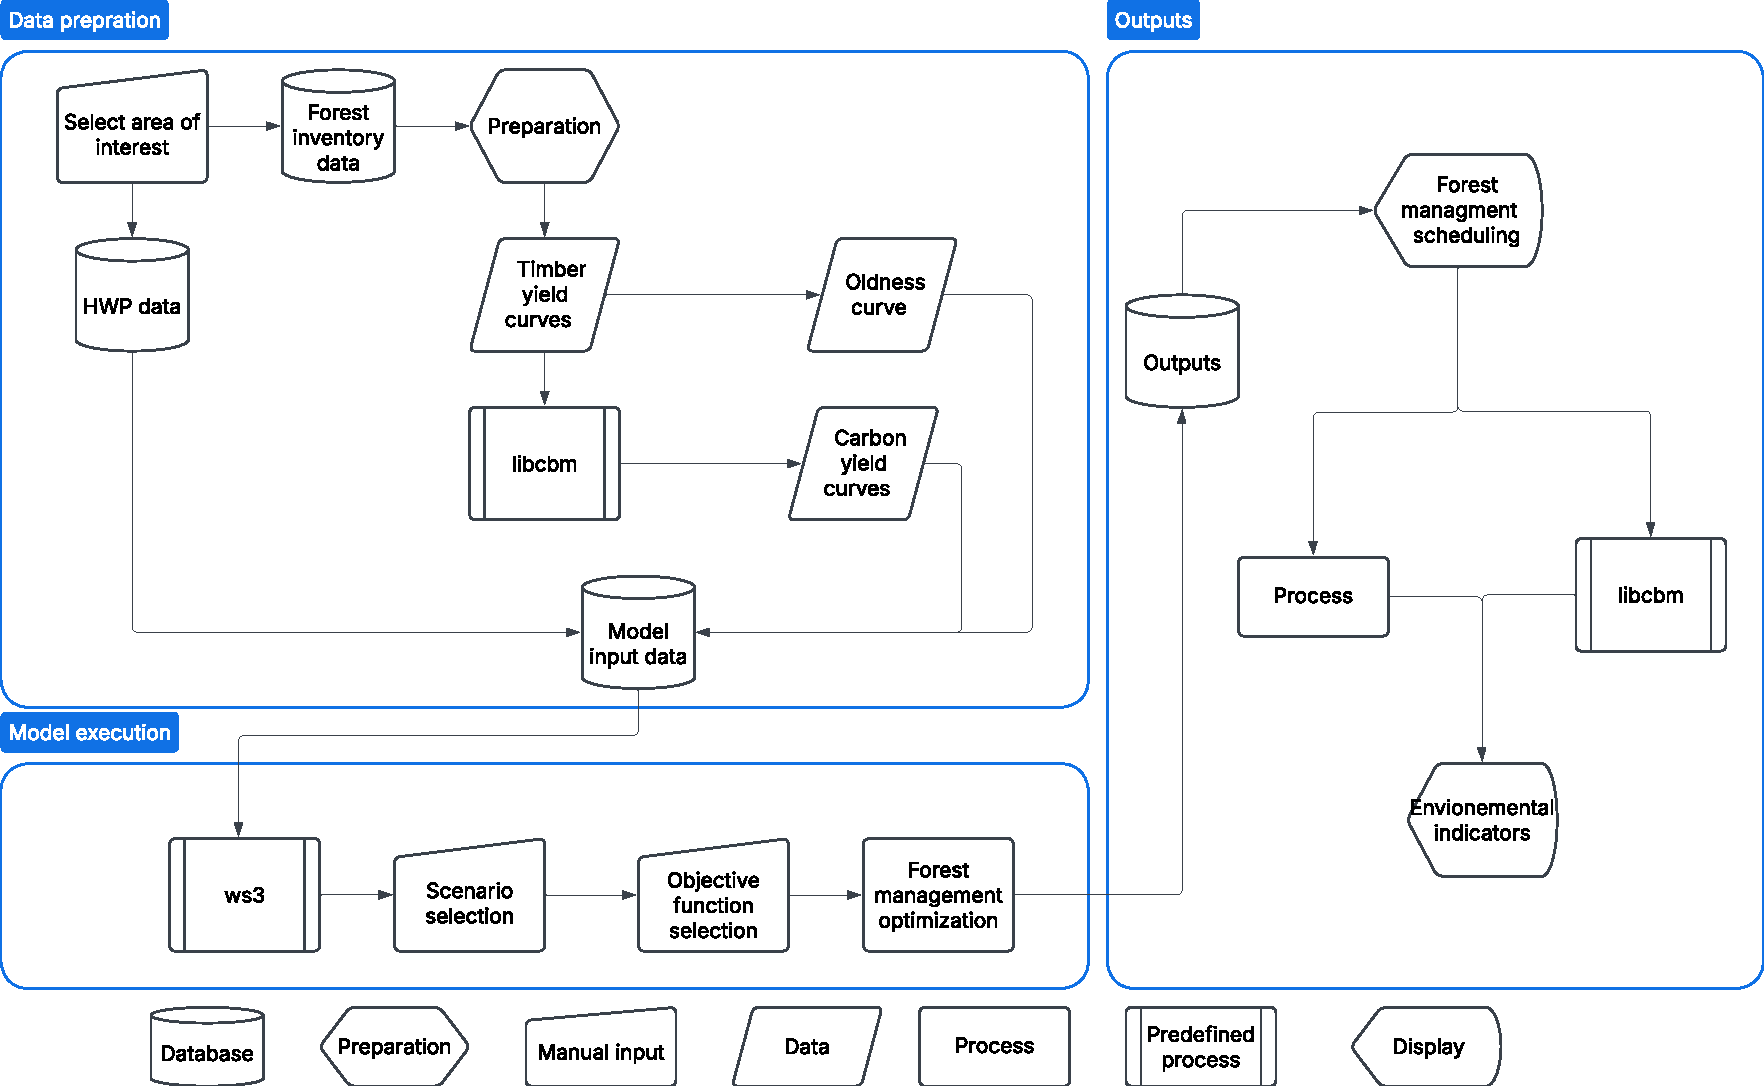
\includegraphics[width=\linewidth]{fig 1.1.pdf} 
    \caption{Overview of the data preparation and model execution process.}
    \label{fig:Fig.1}  
\end{figure}

\subsection{Modeling framework}
\label{sec: model}

This section describes the modeling framework, including the base mathematical formulation and the alternative objective functions considered.

\subsubsection{Mathematical model}
\label{sec: Mathematical model}

The prototype can simulate forest growth and different forest management activities (e.g., harvesting) at the landscape level for long-term horizons. To support planning experiments, a linear programming model adapted from \citet{Paradis2025_ws3_preprint} is employed to optimize harvest scheduling decisions considering initial forest inventory and forest growth and yield curves to achieve certain objectives while satisfying a set of defined constraints.
The proposed model has several notations, input parameters, and variables shown in Table \ref{tab:Notations}.

\begin{table}[H]
\caption{Notations of the model} % Caption placed above the table
\label{tab:Notations} % Place label right after caption
\centering
\begin{tabular}{lp{10cm}} % Define 2 columns (left, paragraph for description)
\hline
\textbf{Notations} & \textbf{Description} \\
\hline
\textit{Sets} &  \\
\hline
$Z$ & Set of spatial zones $i \in Z$ \\

$K$ & Set of available prescriptions $k \in K$ \\
$J$ & Set of forest outputs, $j \in \{1: \text{area}, 2: \text{volume}\}$ \\
$T$ & Set of time periods in the planning horizon \\
\hline
\textit{Parameters} & \\
\hline
$c_{ij}$ & Objective function contribution of prescription $j \in J_i$ in zone $i \in Z$ \\
$\beta_j$ & Admissible level of variation on yield of targeted output $j \in J$ \\
$\alpha_{ikjt}$ & Quantity of output $j \in J$ produced in period $t \in T$ by prescription $k \in K$ in zone $i \in Z$ \\
$l_{jt}$ & Lower bound on yield of output $j \in J$ in period $t \in T$ \\
$u_{jt}$ & Upper bound on yield of output $j \in J$ in period $t \in T$ \\
$y_{j}$ & targeted sustainable yield of output $j \in J$  \\
$gl$ & Lower bound on the volume growth at the end of the planning horizon\\
\hline
\textit{Variables} &  \\
\hline
$I_{jt}$ & Inventory quantity of output $j \in J$ in period $t \in T$\\
$G_{jt}$ & Growth amount of output $j \in J$ in period $t \in T$\\
$x_{ik}$ & Proportion of zone $i \in Z$ on which prescription $k \in K$ is applied
\end{tabular}
\label{tab:model}
\end{table}

The mathematical formulation of the proposed model is as follows:
\begin{align}
\text{max} & \quad \sum_{i \in Z} \sum_{k \in K} c_{ij} x_{ik} \label{eq:1} \\
\text{s.t.} & \quad \sum_{k \in K} x_{ik} = 1, \quad \forall i \in Z \label{eq:2} \\
& \quad y_{j} (1 - \beta_j) \leq \sum_{i \in Z} \sum_{k \in K} \alpha_{ikjt} x_{ik} \leq y_{j} (1 + \beta_j), \quad \forall j \in J, t \in T \label{eq:3} \\
& \quad l_{jt} \leq \sum_{i \in Z} \sum_{k \in K} \alpha_{ikjt} x_{ik} \leq u_{jt}, \quad \forall j \in J, t \in T \label{eq:4} \\
& \quad I_{2t} = I_{2(t-1)} + G_{jt} - \sum_{i \in Z} \sum_{k \in K} \alpha_{ik2t} x_{ik}, \quad \forall t \in T \label{eq:5} \\
& \quad I_{2T} \geq gl \label{eq:6} \\
& \quad 0 \leq x_{ik} \leq 1, \quad \forall i \in Z, k \in K \label{eq:7}
\end{align}
Objective function (\ref{eq:1}) maximizes the desired objective considering the applied prescriptions. Depending on the problem, different objectives can be defined that will be discussed in Section \ref{sec: Objective functions} Constraint set (\ref{eq:2}) implies that total the proportion of prescriptions on each zone should be one. It is noteworthy that doing nothing is a valid prescription along with other prescriptions such as harvesting. Constraints (\ref{eq:3}) are even flow constraints, ensuring consistent target outputs (i.e., harvested volumes and areas). Constraint set (\ref{eq:4}) imposes upper bound and lower bounds on periodic yields. Constraint set (\ref{eq:5}) determines inventory volume for each period including new growth and harvested volume. A lower bound for the inventory volume in the last period is imposed by the constraint set (\ref{eq:6}). Finally, the domain of decision variables is determined by the constraint sets (\ref{eq:7}).

\subsubsection{Objective functions}
\label{sec: Objective functions}
It should be noted that the model is generic and the objective function can be to maximize harvested volume, minimize harvested area, maximize ecosystem carbon stocks, and minimize net carbon emissions.

\emph{Maximize harvested volume.}
This objective aims to maximize the total harvested volume  where the volume of harvested wood is obtained using timber yield curves. Objective function (\ref{eq:8}) aims to maximize the total harvested volume over the planning horizon.
\begin{align}
       \text{max} & \quad \sum_{i \in Z} \sum_{k \in K} \sum_{t \in T} \alpha_{ik2t} x_{ik} \label{eq:8} 
\end{align}

\emph{Minimize harvested area.}
This objective aims to minimze the total harvested area. Objective function (\ref{eq:9}) aims to minimize the total harvested area over the planning horizon.

\begin{align}
       \text{min} & \quad \sum_{i \in Z} \sum_{k \in K} \sum_{t \in T} \alpha_{ik1t} x_{ik} \label{eq:9} 
\end{align}


\emph{Maximize ecosystme carbon stocks.}
Objective function (\ref{eq:10}) tries to maximize amount of carbon stock in the ecosystem, i.e., forest inventory, and HWP. To get the ecosystem carbon stocks, carbon curves are generated by libCBM \citep{libcbmpy} to track biomass and DOM carbon pools. Biomass pools are referred to those carbon stored in living components including roots and merchantable volumes while Dead Organic Matter (DOM) pools include carbon stocks in woody debris and litter \citep{KURZ2009480}.  HWPs are important carbon stocks \citep{geng2017review}, and their half lives are used as a reliable measure to determine carbon storage \citep{braun2016apparent}. Eq. (\ref{eq:11}) is used to determine the periodic carbon stock over the planning horizon, respectively.

\begin{align}
\max \quad & S^{e} + \sum_{p \in P} \sum_{t \in T} S_{pt} \label{eq:10}
\end{align}

\begin{align}
S_{pt} &= \left( \left(1 - \frac{\ln 2}{t_{1/2}^{p}}\right) S_{p(t-1)} + \sum_{i \in Z} \sum_{k \in K} \alpha_{ik2t} x_{ik} \cdot w \cdot n \right) \label{eq:11}
\end{align}

\noindent where:
\begin{align*}
    \text{w} &:= \text{wood density}, \\
    \text{n} &:= \text{carbon content}, \\
    \text{P} &:= \text{set of HWP } p \in P, \\
    \text{S}^{e} &:= \text{carbon retained in the ecosystem}, \\
    \text{S}_{pt} &:= \text{carbon stock in HWP } p \text{ in period } t , \\
    t_{1/2}^{p} &:= \text{half-life of the HWP }p \in P.
\end{align*}

\emph{Minimize net emissions.}
   Objective function (\ref{eq:12}) minimizes total emissions considering ecosystem emissions, HWPs decay and displacement effects.
   The ecosystem emissions are obtained from libCBM \citep{libcbmpy} while emissions from decaying HWPs are calculated using their half lives. Additionally, these HWPs have displacement effects, avoiding emissions by replacing other GHG-intensive products \citep{geng2017review}. Periodic emissions from HWPs decay and displacement over the planning horizons are calculated using Eqs. (\ref{eq:13}) and (\ref{eq:14}) respectively.
   
\begin{align}
   \min & \quad E^{e} + \sum_{p \in P} \sum_{t \in T} E_{pt} - \sum_{d \in D} \sum_{t \in T} E_{dt}
   \label{eq:12}
\end{align}   
\begin{multline}
    E_{pt} = \left( (1 - \frac{ln 2}{t_{1/2}^{p}}) \times 
    \sum_{i \in Z} \sum_{k \in K} \alpha_{ik2t} x_{ik} \times \text{m}_{p} \times \text{w} \right. \\
    \left. \times \text{n} \times \frac{44}{12} \right)
    \label{eq:13}
\end{multline}
\begin{multline}
    E_{dt} = \left( \sum_{i \in Z} \sum_{k \in K} \sum_{p \in P} \alpha_{ik2t} x_{ik} \times \text{m}_{p} \times r_{pd} \times \left(1 - \frac{\ln 2}{t_{1/2}^{p}}\right) \right. \\
    \left. \times \text{f} \times \text{w} \times \text{n} \times \frac{44}{12} \right)
    \label{eq:14}
\end{multline}
  
\noindent where:
\begin{align*}
    \text{D} &:= \text{set of products replaced by HWPs}, d \in D, \\
    \text{f} &:= \text{displacement factor}\\
    \text{E}^{e} &:= \text{carbon emissions released by the ecosystem}, \\
    \text{E}_{pt} &:= \text{carbon emissions released by HWP } p \in P \text{ in period } t \in T \\
    \text{E}_{dt} &:= \text{carbon emissions avoided when } d \in D \text{ is replaced by HWP }p \in P \\
    \text{r}_{pd} &:= \text{percentage of HWP } p \in P \text{ that would replace product } d \in D, \\
    \text{m}_{p} &:= \text{percentage of harvest amount converted to HWP } p \in P
    \end{align*}

\subsection{Environmental indicators}
\label{sec: indicators}
Outputs from the prototype framework include a set of KPI spanning environmental aspects, allowing evaluation of forest management practices under various scenarios and management objectives in our case studies. 

Most of the studies conducted in the past focused on the various environmental impacts of forest management activities \citep{Seely2002, KURZ2009480, Valipour2021, Boisvenue2022}. In the prototype developed in this study, carbon stocks are evaluated as part of environmental indicators in multiple pools, including total carbon of the ecosystem (biomass and DOM) and HWP.
Net emissions are calculated by considering emissions from ecosystem and HWP decay, while accounting for carbon removals from forest growth and the displacement effect of HWP. 

Other environmental KPIs in this are related to biodiversity concerns. The biodiversity of forested ecosystems significantly influences the long-term carbon storage dynamics \citep{Diaz2009}. In \citet{Diaz2006}, biodiversity is defined as the number, abundance, composition, spatial distribution and interactions of genotypes, populations, species, functional types, traits, and landscape units within a given system. However, in this study, we measured biodiversity by evaluating the diversity of tree species and the characteristics of old growth, quantified using the Shannon Evenness Index (SEI) \citep{Gergel2017} and the old growth yield curve generated in this study, respectively. \citet{McGarvey2015} modeled the relationship between carbon stocks and the age of the oldest trees using linear regression. Their findings illustrate that old-growth forests have stored more carbon. 

The Shannon Evenness Index (\(SEI\)) is calculated as Eq. (\ref{eq:15}):
\begin{equation}
SEI = \frac{-\sum_{i=1}^{S} p_i \ln p_i}{\ln S}
\label{eq:15}
\end{equation}
where \( S \) is the total number of species (species richness), and \( p_i \) is the proportion of individuals belonging to species \( i \).
The SEI yields a value between 0 and 1, where 1 indicates complete evenness in species distribution. A higher Shannon Index Evenness value reflects greater biodiversity, indicating a more balanced distribution of tree species within the forest.

The framework calculates the Old Growth Index (OGI) by modeling forest age distribution and volume growth. As shown in Eq.(\ref{eq:16}), the index is defined as a piecewise function where the OGI value is zero for younger forest ages, linearly interpolates between specified age thresholds, and reaches a maximum value of 1 for older forests, reflecting the progression towards old-growth conditions.

\begin{equation}
\label{eq:16}
f(x) = 
\begin{cases}
  0 & \text{if } a \leq \Delta_1 a^* + \Delta_2 \\
  \dfrac{a - (\Delta_1 a^* + \Delta_2)}{(\Delta_3 a' + \Delta_4) - (\Delta_1 a^* + \Delta_2)} & \text{if } \Delta_1 a^* + \Delta_2 < a < \Delta_3 a' + \Delta_4 \\
  1 & \text{if } a \geq \Delta_3 a' + \Delta_4
\end{cases}
\end{equation}


where $a$, $a^*$, and $a^{\prime}$ denote the age of the stand, the rotation age (the optimal age at which a forest stand is harvested to maximize timber yield), and the age of maturity (i.e., the age when the stand or tree reaches its peak growth or maximum yield before decline), respectively. The parameters $\Delta_1$, $\Delta_2$, $\Delta_3$, and $\Delta_4$ represent arbitrary values used to adjust the age thresholds. For the case study presented here, we use $\Delta_1 = \Delta_3 = 1$ and $\Delta_2 = \Delta_4 = 0$.

\subsection{Computational setup}
\label{Computational}
The prototype implementation is in Python, with the model interface designed within a Jupyter notebook running in a JupyterLab environment. It was developed and tested on a cloud-based virtual machine running Ubuntu Linux 24. The current notebook-based interface is intentionally simple and not optimized for end users, but it supports full transparency, reproducibility, and observability of the analysis pipeline. The framework is designed to be portable across computing environments, including desktop computers running Microsoft Windows. Future development could improve usability (e.g., CLI or GUI) while preserving open, auditable workflows.

\section{Case study}
\label{sec: Case Study}
\subsection{Study area}
\label{sec: Study area}
The mining company considered in this study operates several active and legacy mining sites across Canada. Legacy mine sites are locations where mining previously took place but is no longer active \citep{worrall2009towards}. In this study we focus on three mining sites in British Columbia (BC), Canada, including two legacy sites and one active site, as a case study. 
Figure \ref{fig:Fig.2} illustrates the Area of Interest (AOI) for the mining sites, while Table \ref{tab:area} details their Timber Supply Areas (TSA), and area specifications. A TSA is ``a designated area established by the BC Ministry of Forests in order to practice sound, integrated, resource management principles to improve the allowable annual cuts"\citep{CanadaOpenData2025}. The study area for Mining Site 1 is located in the northwest-central region of BC, spanning 1,137,000 hectares and encompassing parts of the Bulkley, Kispiox, Lakes, Morice, and Prince George TSAs. The study area surrounding Mining Site 2, located in the northwestern part of BC, falls within the Cassiar TSA, covering approximately 538,000 hectares. The study area for Mining Site 3, also situated in the northwestern region of BC, is within the Cassiar TSA, encompassing about 405,000 hectares. 

Figure \ref{fig:Fig.2} shows the location of the mining sites and the surrounding watersheds used to define the AOI. The watershed containing the mine location is identified as the primary watershed, the adjacent watersheds as secondary, and watersheds neighboring the secondary ones as tertiary. This structure creates a hierarchical framework of watersheds surrounding each mine site. The watershed was chosen as the basis for defining the AOIs because it is a meaningful ecological spatial unit, with its size and shape related to local ecosystem boundaries and gradients \citep{flotemersch2016watershed}. While watersheds were used to define the AOI, other landscape features could also serve this purpose. This method was selected with the intention that future studies could vary management intensity across the different watershed levels. The prototype framework presented here could also work with AOIs defined using alternative criteria. The colored areas represent the Timber Harvesting Land Base (THLB, in green), forested non-contributing areas (in yellow), and excluded zones (in gray) within each AOI, providing context for land classifications surrounding each site. The THLB is an estimate of the land where timber harvesting is both acceptable and economically feasible \citep{bcgov2025}. Poor and non-productive forest lands are classified as forested non-contributing areas, while non-forested lands such as roads, rivers, wetlands, and lakes are excluded from the AOI.

\begin{table}[H]
\centering
\caption{Mining sites and areas}
\label{tab:area}
\begin{adjustbox}{width=\textwidth}
{\small
\begin{tabular}{lllrrr}
\toprule
\makecell[l]{Mining\\Site} & 
\makecell[l]{Site\\Status} & 
\makecell[l]{Timber\\Supply\\Areas (TSAs)} & 
\makecell[r]{Excluded\\Area\\(k ha)} & 
\makecell[r]{Non-\\contrib.\\Area (k ha)} & 
\makecell[r]{THLB\\Area\\(k ha)} \\
\midrule
Mining Site 1 & Legacy & \makecell[l]{Bulkley, Kispiox,\\ Lakes, Morice,\\ Prince George} & 225.1 & 249.3 & 662.9 \\
Mining Site 2 & Legacy & Cassiar & 347.1 & 56.5 & 134.7 \\
Mining Site 3 & Active & Cassiar & 13.9 & 202.1 & 188.7 \\
\bottomrule
\end{tabular}
}
\end{adjustbox}
\end{table}


\begin{figure}[H]
    \centering
    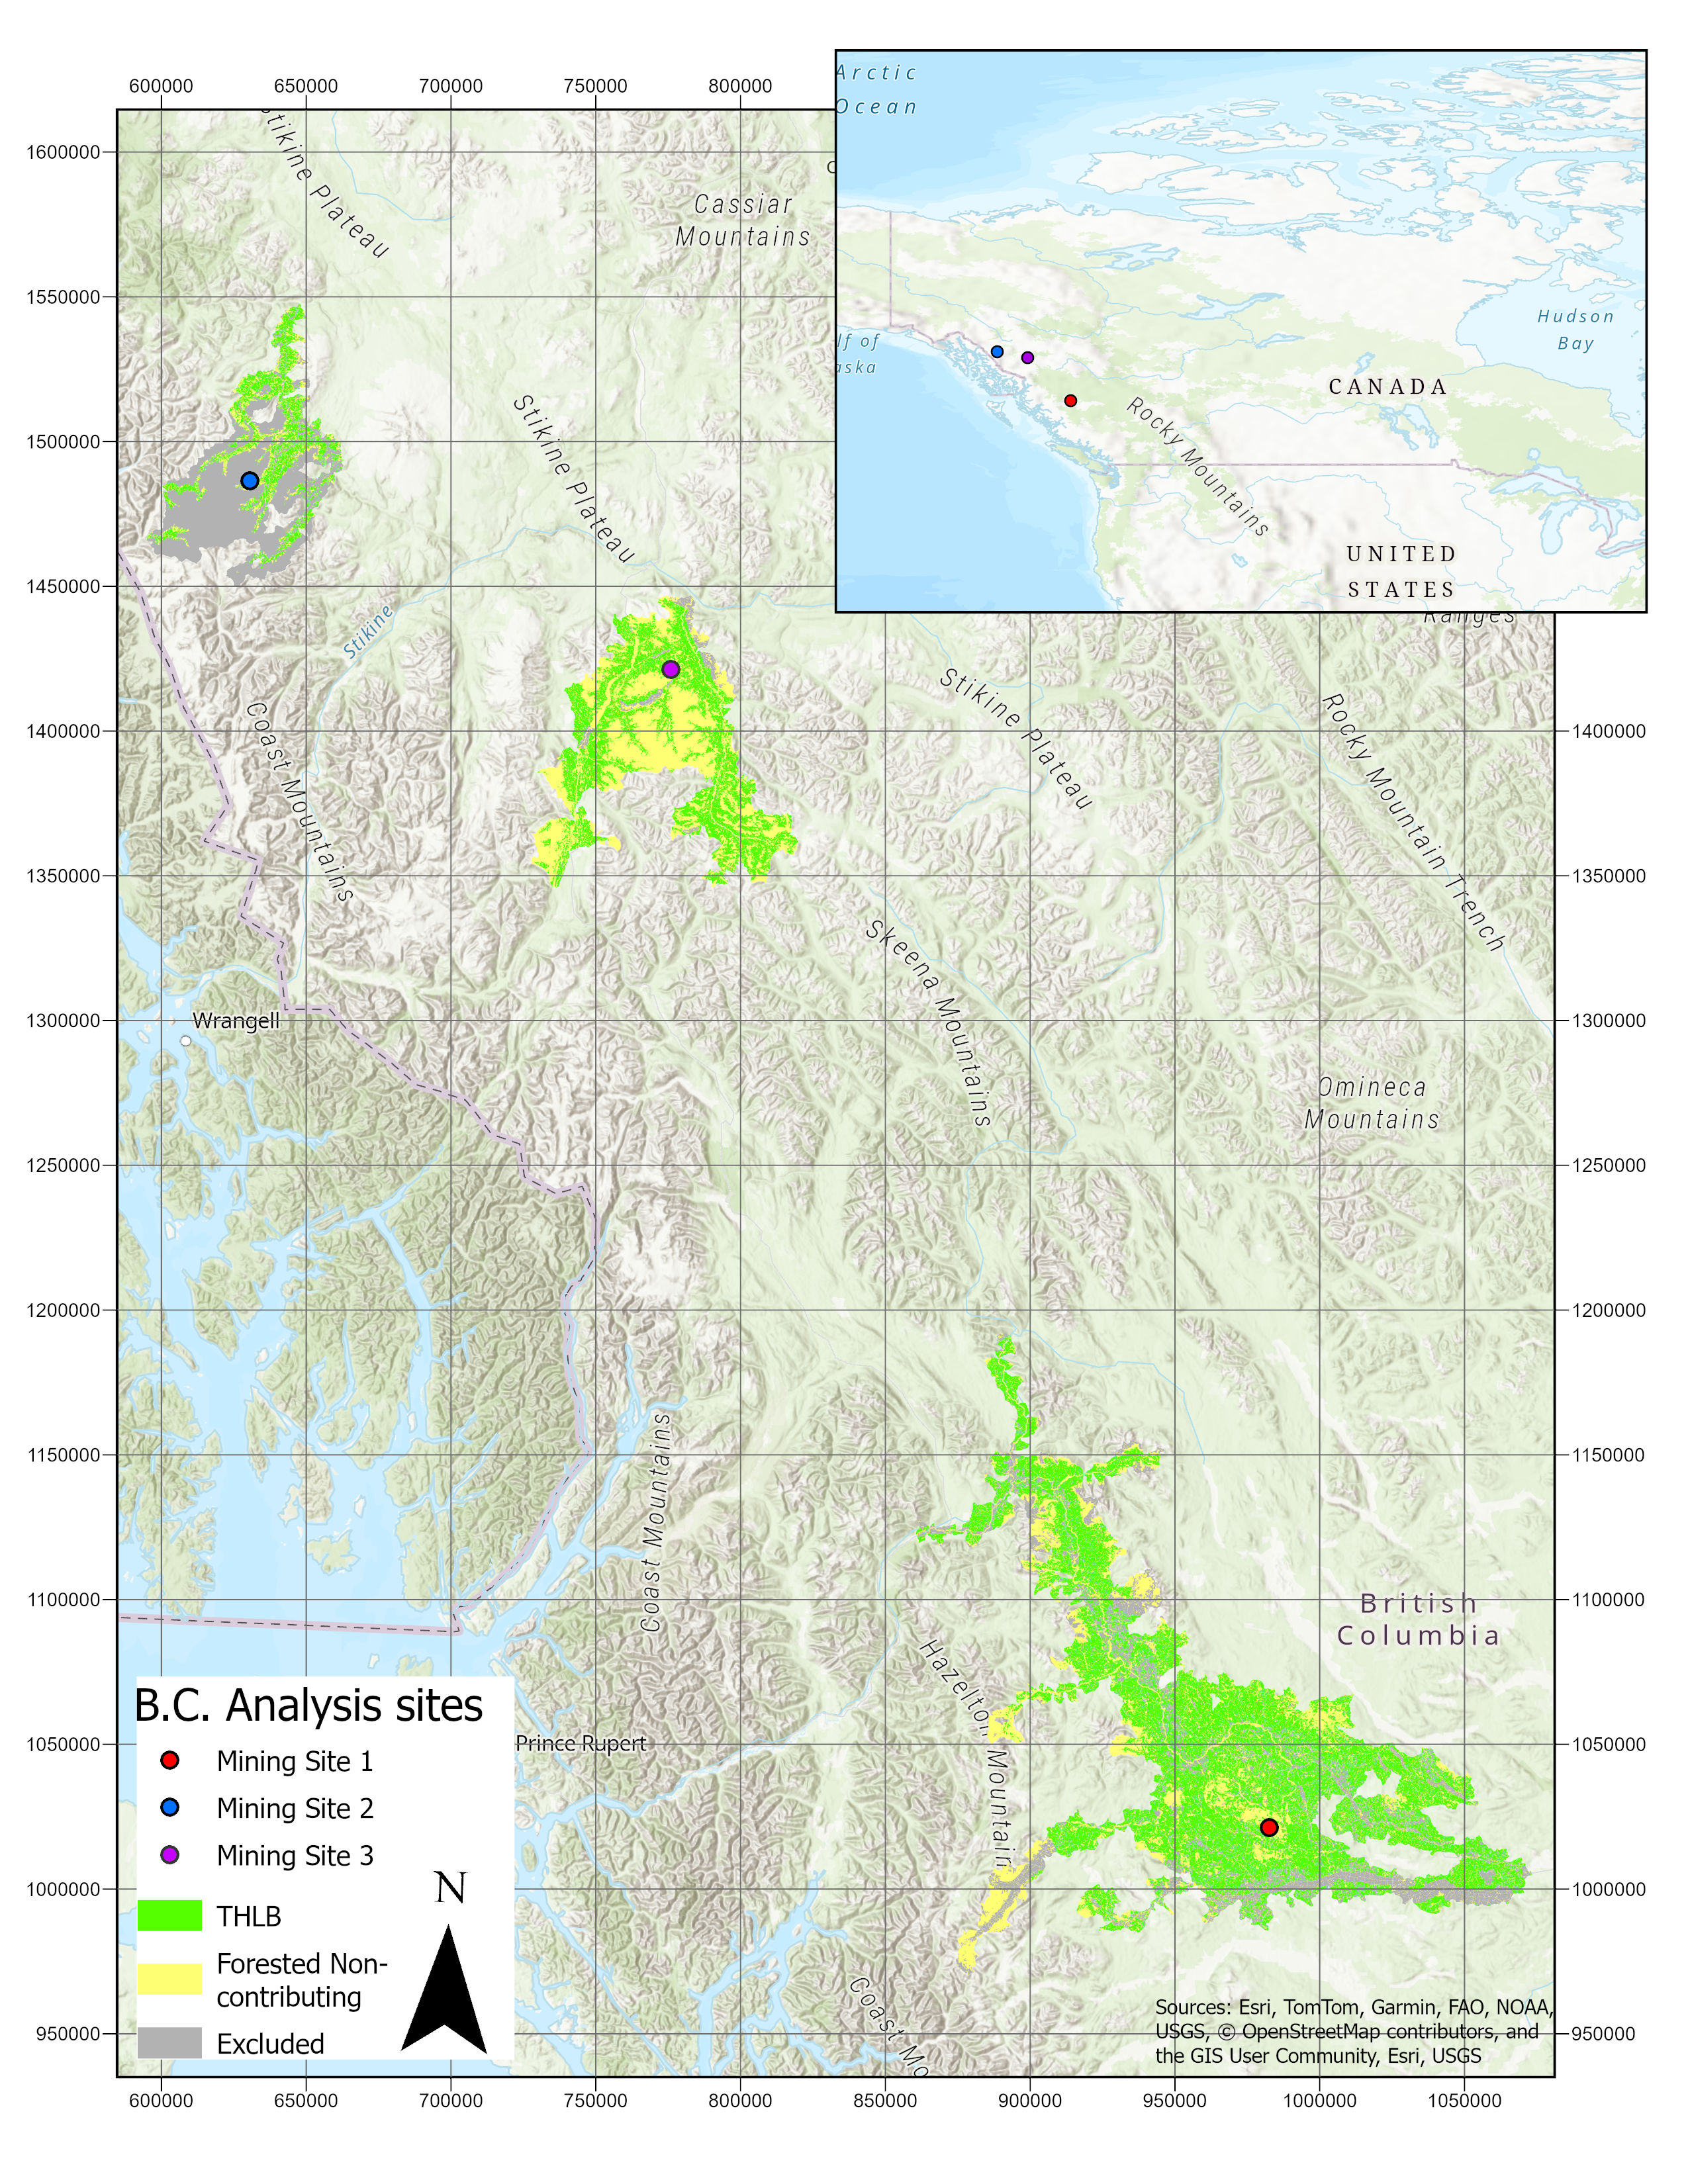
\includegraphics[width=\linewidth]{Fig.2.jpg} 
    \caption{Location of mining sites in British Columbia and their AOI.}
    \label{fig:Fig.2}    
\end{figure}



\subsection{Data}
\label{sec:data}
Apart from the mining site locations, all other input data used in this study are publicly available, primarily sourced from the BC Government Public Portal (DataBC or the Data Catalogue). The prototype framework requires various input data, including the initial forest inventory, growth and yield curves, carbon stock and emission curves, as well as assumptions regarding HWP allocation to product streams, HWP decay rates, and displacement effects. 

This study utilizes publicly available BC Vegetation Resource Inventory (VRI) datasets to populate the forest stand inventory. Each forest stand is represented by the growth curve of its dominant species, with both hardwood and softwood components modeled using individual growth data. In BC, the Table Interpolation Program for Stand Yields (TIPSY) and the Variable Density Yield Projection (VDYP) models are the standard tools for estimating timber yield projections in managed and natural stands, respectively \citep{BCGov_ForestInventory}. To simulate tree growth dynamics in this study, timber yield curves are generated using the VDYP model.
We employ the default Canadian parameters for libCBM \citep{KURZ2009480}, ensuring alignment with our study area. To analyze carbon stocks and emissions, carbon stock and emissions curves were derived from libCBM to model carbon dynamics over time, building upon the carbon yield curve method originally developed by \citet{neilson2008optimal} and more recently adapted for ws3 and libCBM by \citet{yan2025mathematical}.
To track old growth forest, oldness curves are generated using Eq. (\ref{eq:16}), considering yield curves and rotation age to assess the distribution of the stand age over different periods. Similar to \citet{Ke2024}, the Life Cycle Analysis (LCA) method is employed to track emissions from HWP using the same parameters.

\subsection{Forest management scenarios}
\label{sec: Developed scenarios}
While forest management includes a wide range of activities, our analysis specifically focuses on harvest scheduling as a key component. We develop two sets of management scenarios: a business-as-usual baseline and alternative scenarios. In the business as usual scenario, harvest scheduling is optimized by considering even-flow constraints on harvested area and volume, allowing for a 5\% variation, as well as upper bounds on harvest intensity and lower bounds on growing stock. For growing stock, we assume that the final forest inventory at the end of the planning horizon is not less than 90\% of the initial inventory. To determine the maximum harvest level for areas surrounding mining sites under the baseline scenario, we apply the annual allowable cut (AAC) concept used in BC. The AAC for each TSA is determined by the Chief Forester at least once every ten years \citep{BCForestApportionment}. Since AAC and THLB are predetermined for each TSA, we calculate the maximum harvested volume for each mining site based on the proportion of its THLB relative to the corresponding TSA. In alternative scenarios, the intensity of harvest decreases by 10\%. We coupled these scenarios with an additional scenario that examines the model's behavior when only even-flow constraints on harvested volume and area are considered. Hence, a suite of 11 scenarios was developed for this analysis. All scenarios are modeled over a 100-year planning horizon, divided into 10 periods of 10 years each. Clear-cutting was the only harvesting system used. Table \ref{tab:scenario_constraints} provides an overview of the scenarios included in the analysis.

\begin{table}[H]
\caption{Scenarios and applied constraints}
\centering
\label{tab:scenario_constraints}
\resizebox{\textwidth}{!}{%
{\small
\begin{tabular}{llccc}
\toprule
\makecell[l]{Scenario} & 
\makecell[l]{Scenario\\ID} & 
\makecell[l]{Even-flow constraints\\(area \& volume)} & 
\makecell[l]{Maximum harvested volume\\constraint} & 
\makecell[l]{Growing stock\\constraint} \\
\midrule
Baseline    & Baseline & * & *                  & * \\
Scenario 0  & S0       & * & --                 & -- \\
Scenario 1  & S1       & * & 90\% of Baseline   & * \\
Scenario 2  & S2       & * & 80\% of Baseline   & * \\
Scenario 3  & S3       & * & 70\% of Baseline   & * \\
Scenario 4  & S4       & * & 60\% of Baseline   & * \\
Scenario 5  & S5       & * & 50\% of Baseline   & * \\
Scenario 6  & S6       & * & 40\% of Baseline   & * \\
Scenario 7  & S7       & * & 30\% of Baseline   & * \\
Scenario 8  & S8       & * & 20\% of Baseline   & * \\
Scenario 9  & S9       & * & 10\% of Baseline   & * \\
\bottomrule
\end{tabular}%
}
}
\end{table}


\section{Results}
\label{sec: Results}
\subsection{Parameter initialization}
\label{sec:Parameter initialization }
The prototype is designed to be flexible and can accommodate different planning horizons and period lengths. We analyzed the baseline and alternative scenarios described in Section \ref{sec: Developed scenarios} (S0 to S9) for the three mining sites with four objectives: maximizing harvested volume, minimizing harvested area, maximizing ecosystem carbon stocks, and minimizing carbon net emissions.

Although the prototype can account for various HWPs in different proportions with minor configuration changes, this study focuses on two primary products derived from harvested wood: lumber and paper. Based on historical data on log availability and usage in BC in 2020, 50\% of the logs produced are allocated to solid wood products, while the remaining 50\% are designated for paper production \citep{BC_Mill_List_2020}. However, for the purpose of this study, we assume that 80\% of the harvested wood is converted into lumber and 20\% into paper. This assumption allows us to explore harvesting scenarios under the condition that a greater portion of harvested wood is dedicated toward products with longer life cycles. As stated by the IPCC, paper typically has a half-life of up to 2 years, whereas wood-based panels have a half-life of up to 25 years, and sawnwood has a half-life of 35 years \citep{Brunet-Navarro2016}. Therefore, in this study, a half-life of 30 years is assigned to lumber, while paper is given a half-life of 2 years. Furthermore, to account for the substitution effect, we assume that 50\% of the lumber is processed into cross-laminated timber (CLT), which has a long-term carbon displacement impact due to its extended lifespan, estimated at around 100 years according to \citet{head2020dynamic} and is considered effectively permanent for the purposes of this study. Since our primary objective was to demonstrate the applicability of the prototype rather than to generalize the results, we did not conduct a sensitivity analysis on these parameters. The parameter values employed in this study are reported in \ref{sec:appendix1}

The following subsections offer a detailed analysis of the prototype’s outputs for Mining Site 1, while results for Mining Sites 2 and 3 are provided in \ref{sec:appendix2} and \ref{sec:appendix3}, respectively. These analyses are presented as demonstrations of the framework across sites with differing forest ecosystem dynamics.

\subsection{Harvesting scenarios across planning objectives}
\label{sec: comparison scenarios/objectives}
The results show that decisions related to harvest scheduling are sensitive to the selected objective. Figure \ref{fig:Fig.3} compares harvested area, harvested volume, and growing stock in the forest lands surrounding Mining Site 1 under the baseline scenario and scenario S0 (which includes only even-flow constraints), across four key objectives: maximizing harvested volume (\text{Max\_hv}), minimizing harvested area \text{Min\_ha}), maximizing ecosystem carbon stocks (\text{Max\_st}), and minimizing net carbon emissions (\text{Min\_em}).

For the objective of maximizing harvested volume, scenario S0 results in higher harvested area and harvested volume compared to the baseline. Growing stock under scenario S0 declines more over the planning horizon, indicating more intensive harvesting. Notably, S0 shows increased harvesting levels toward the end of the planning horizon, reflecting an effort to maximize wood resource extraction over time. Under the ecosystem carbon stocks maximization objective, the prototype suggests no harvesting at all in scenario S0. This leads to a substantially higher growing stock, highlighting the system’s preference for carbon accumulation when not constrained by harvesting targets. Similar results are observed under the objective of minimizing harvested area, where the model avoids harvesting entirely to preserve standing biomass. For the objective of minimizing net emissions, harvested area and volume under scenario S0 are significantly lower across all periods compared to the baseline. However, based on the initialized parameters, the prototype recommends a low level of harvesting under the scenario S0. The difference in outcomes between the scenario S0 under  carbon stock maximization and net emissions minimization is likely due to the displacement effect, which reduces the impact of harvest-related emissions by assuming they are offset through substitution.

It is also important to examine the behavior of the baseline scenario, which includes harvesting targets applied uniformly across all objectives. Although the same constraints on harvested area, volume, and growing stock are imposed under each objective, the outcomes differ. Harvested volume remains relatively consistent across objectives, reflecting the need to meet predefined volume targets. However, this consistency does not extend to harvested area, where notable variations are observed. These differences may be attributed to the diverse growth rates of tree species and their varying contributions to biomass pools and DOM. Consequently, the harvested area may vary depending on the species composition prioritized under different management objectives.

Figure \ref{fig:Fig.4} illustrates how different management objectives influence the species composition of retained stands under the baseline scenario. It compares the distribution of tree species at the end of the planning horizon across four harvesting objectives, alongside a no-harvest case that reflects the initial inventory composition.
Retention patterns for Western Hemlock (\textit{Tsuga heterophylla}), Douglas-fir (\textit{Pseudotsuga menziesii}), Trembling Aspen (\textit{Populus tremuloides}), and Spruce and Spruce Hybrids (\textit{Picea}) remain relatively consistent across objectives, with Western Hemlock and Spruce showing slightly higher retention under the maximize carbon stock objective. Pines (\textit{Pinus}) emerges as the dominant retained species under the minimize emissions objective. In contrast, Balsam (\textit{Abies lasiocarpa}) dominates under the maximize carbon stock objective.

\begin{figure}[H]
    \centering
    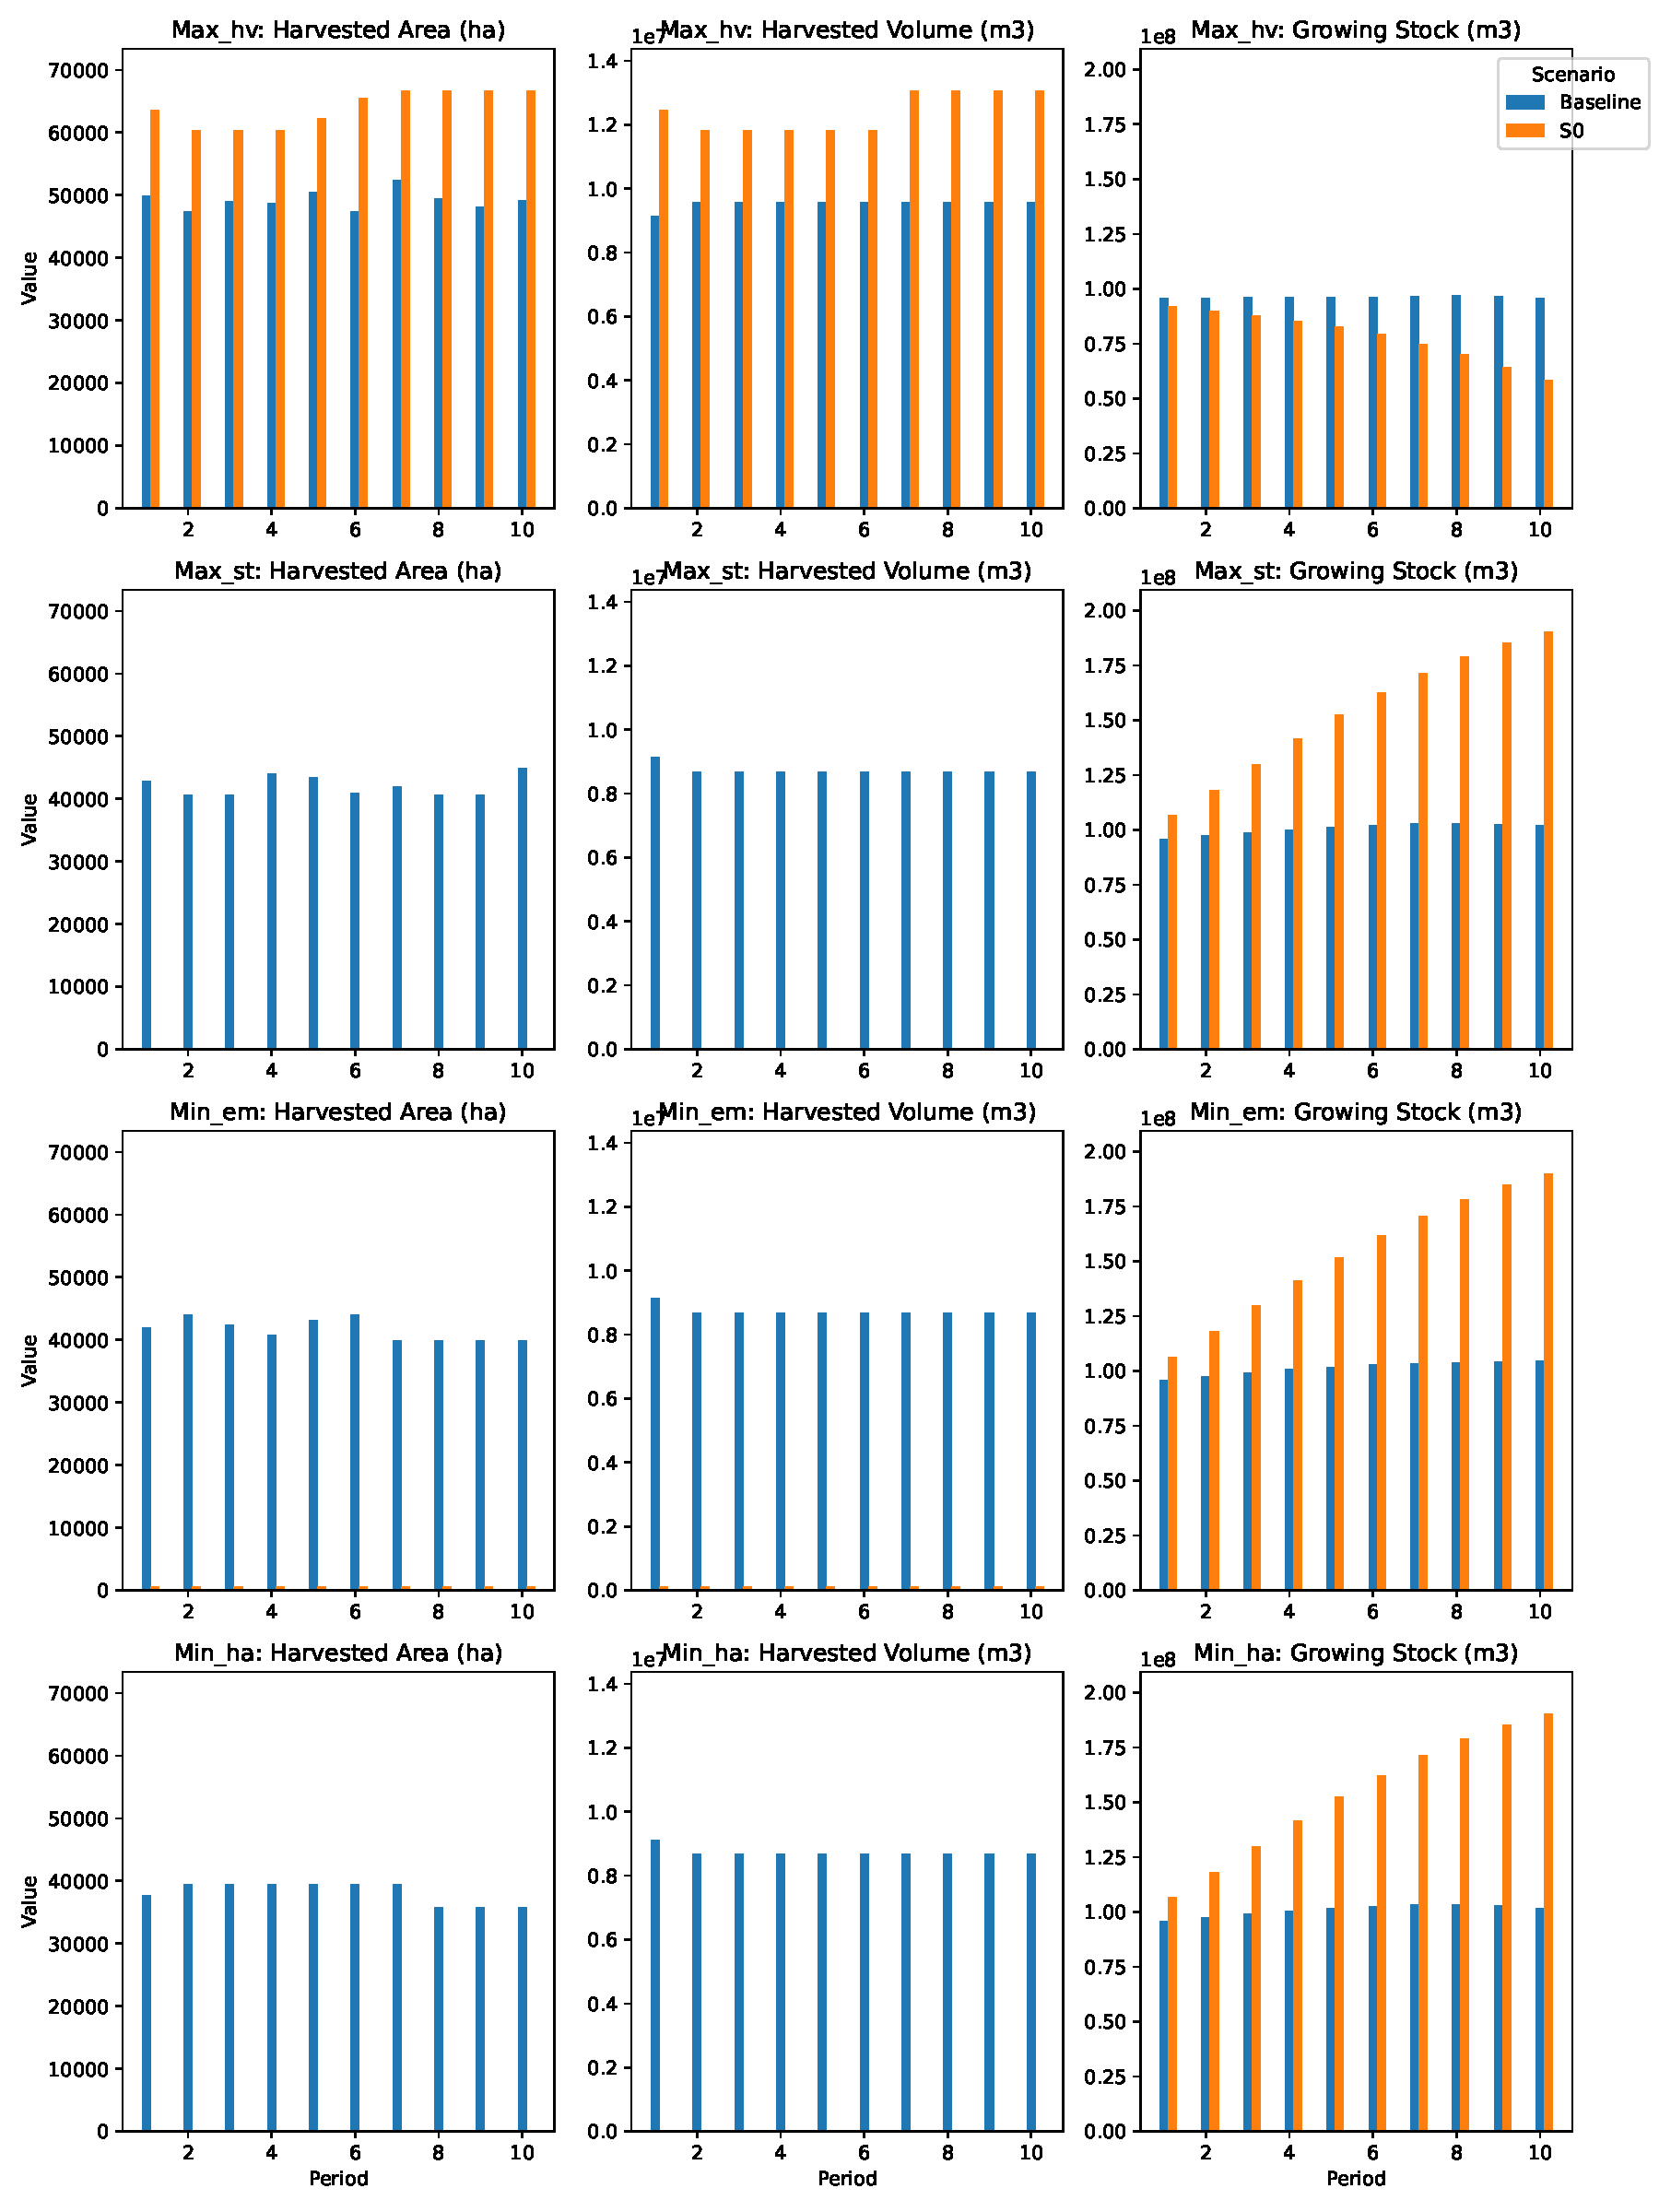
\includegraphics[width=\linewidth]{Fig.3.pdf} 
    \caption{Comparison of harvested area, volume, and growing stock in the forest lands surrounding Mining Site 1: Baseline vs. scenario S0 across planning objectives.}
    \label{fig:Fig.3}    
\end{figure}

\begin{figure}[H]
    \centering
    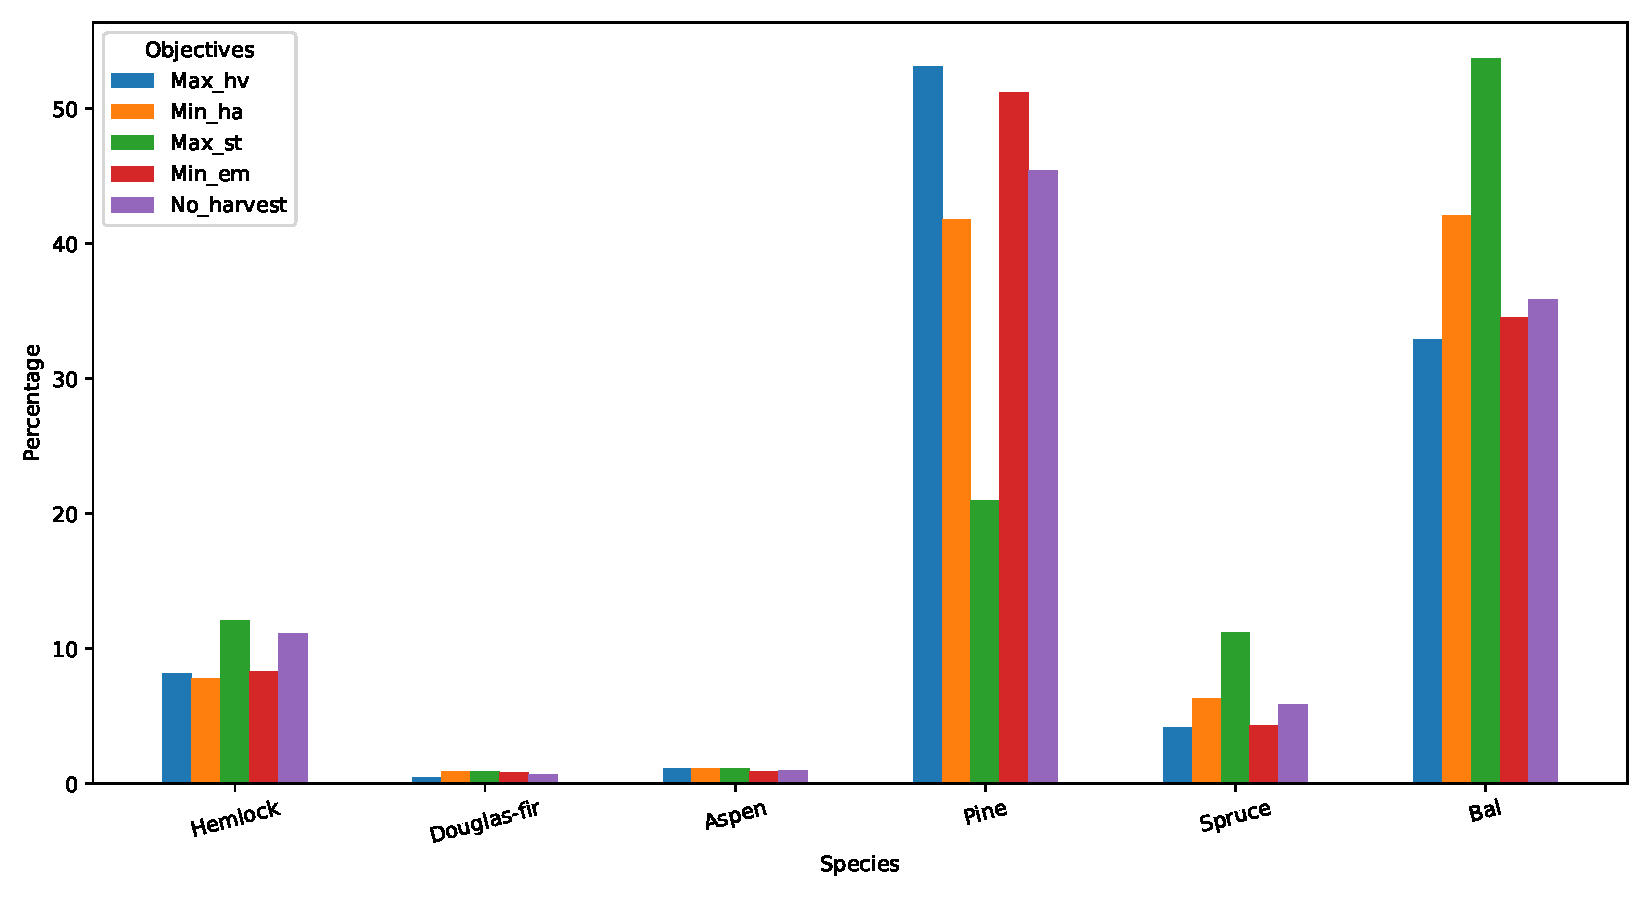
\includegraphics[width=\linewidth]{Fig.4.pdf} 
    \caption{Comparison of retained tree species under planning objectives and the no-harvest condition in forest lands surrounding Mining Site 1 (baseline scenario).}
    \label{fig:Fig.4}    
\end{figure}

\subsection{Environmental KPIs across harvesting scenarios under different planning objectives}
\label{sec: KPIs}
Forest management decisions are not only shaped by the objectives we choose, but they can also have varying impacts on environmental KPIs.
Tables \ref{tab:KPIs_max_hv} to \ref{tab:KPIs_min_ha} show the comparison of the baseline and alternative scenarios (S0 to S9) across the environmental KPIs, considering the objectives of maximizing harvested volume (\text{Max\_hv}), minimizing harvested area \text{Min\_ha}), maximizing carbon stock (\text{Max\_st}), and minimizing net emissions (\text{Min\_em}) for the forest lands surrounding Mining Site 1.

Under the objective of maximizing harvested volume, Scenario S0 results in high elevated harvest levels. However, this comes at the expense of environmental performance, with lower scores in the old-growth and net emissions indicators, reflecting increased carbon emissions and loss of old-growth forest. As harvested volume restrictions become more stringent in scenarios such as S1 and S2, harvest levels decline accordingly, leading to notable improvements in both net emissions and old-growth preservation. Scenario S9, with the lowest harvested volume under this objective, demonstrates the strongest performance on these environmental indicators.

Species diversity shows minimal variation across scenarios regardless of the objective. Scenario S1, which allows for 90\% of the baseline harvested volume, achieves the highest value. However, no consistent trend is observed between harvested volume and species diversity, as values fluctuate across scenarios.
While harvested volume decreases linearly across scenarios, this linear pattern does not hold for net emissions, species diversity, or old-growth indicators.

Under the objectives of maximizing ecosystem carbon stocks, minimizing net emissions, and minimizing harvested area, the baseline scenario shows the highest harvested volume. However, it also produces the highest net emissions and results in the lowest area of old-growth forest. From an environmental and biodiversity standpoint, Scenario S0 (which entails the lowest or no harvesting under these objectives) performs best, offering the greatest carbon retention and preservation of old-growth forest.

Similar to the patterns observed under the maximizing harvested volume, no clear relationship is evident between harvest levels and species diversity, with values varying irregularly across scenarios.

In the following subsections, we analyze the performance of each KPI across different scenarios and management objectives in the forested lands surrounding Mining Site 1.

\begin{table}[H]
\centering
\caption{Comparison of KPIs across harvesting scenarios for the forest lands surrounding Mining Site 1 under the objective of maximizing harvested volume}
\label{tab:KPIs_max_hv}
\begin{adjustbox}{width=\textwidth}
{\small
\begin{tabular}{lrrrr}
\toprule
\makecell[l]{Scenario} & 
\makecell[r]{Harvest\\Volume\\($\mathrm{Mm}^3$)} & 
\makecell[r]{Net\\Emissions\\(MtCO\textsubscript{2}e)} & 
\makecell[r]{Species\\Indicator} & 
\makecell[r]{Old\\Growth\\(k ha)} \\
\midrule
Baseline &  95.4 &  -10.2 &  0.733 & 196.4 \\
S0       & 123.8 &   44.2 &  0.758 & 167.1 \\
S1       &  85.8 &  -20.2 &  0.761 & 222.9 \\
S2       &  76.3 &  -37.7 &  0.751 & 247.4 \\
S3       &  66.8 &  -53.6 &  0.745 & 286.9 \\
S4       &  57.2 &  -69.0 &  0.740 & 324.9 \\
S5       &  47.7 &  -83.7 &  0.738 & 367.4 \\
S6       &  38.2 &  -96.9 &  0.728 & 420.2 \\
S7       &  28.6 & -116.5 &  0.733 & 462.8 \\
S8       &  19.1 & -127.3 &  0.737 & 502.6 \\
S9       &   9.5 & -141.6 &  0.740 & 535.5 \\
\bottomrule
\end{tabular}
}
\end{adjustbox}
\end{table}

\begin{table}[H]
\centering
\caption{Comparison of KPIs across harvesting scenarios for the forest lands surrounding Mining Site 1 under the objective of minimizing harvested area.}
\label{tab:KPIs_min_ha}
\begin{adjustbox}{width=\textwidth}
{\small
\begin{tabular}{lrrrrr} % first column left aligned
\toprule
\makecell[l]{Scenario} & 
\makecell[r]{Harvest\\Volume\\($\mathrm{Mm}^3$)} & 
\makecell[r]{Harvest\\Area\\(k ha)} & 
\makecell[r]{Net\\Emissions\\(MtCO\textsubscript{2}e)} & 
\makecell[r]{Species\\Indicator} & 
\makecell[r]{Old Growth\\(k ha)} \\
\midrule
Baseline & 86.0 & 381.9 &  -27.5 & 0.754 & 303.7 \\
S0       & -    & --    & -155.6 & 0.746 & 580.5 \\
S1       & 77.7 & 333.3 &  -42.3 & 0.753 & 334.1 \\
S2       & 69.3 & 287.4 &  -55.5 & 0.749 & 364.7 \\
S3       & 61.0 & 244.0 &  -69.2 & 0.747 & 393.7 \\
S4       & 52.7 & 203.3 &  -83.3 & 0.744 & 423.1 \\
S5       & 44.4 & 164.5 &  -96.5 & 0.746 & 451.2 \\
S6       & 36.1 & 126.8 & -109.0 & 0.743 & 479.4 \\
S7       & 25.0 &  90.6 & -121.8 & 0.749 & 505.1 \\
S8       & 16.6 &  57.4 & -133.9 & 0.749 & 530.3 \\
S9       & 8.3  &  27.2 & -144.8 & 0.750 & 556.6 \\
\bottomrule
\end{tabular}
}
\end{adjustbox}
\end{table}

\begin{table}[H]
\centering
\caption{Comparison of KPIs across harvesting scenarios for the forest lands surrounding Mining Site 1 under the objective of maximizing carbon stock}
\label{tab:KPIs_max_st}
\begin{adjustbox}{width=\textwidth}
{\small
\begin{tabular}{lrrrrr} % First column left-aligned
\toprule
\makecell[l]{Scenario} & 
\makecell[r]{Harvest\\Volume\\($\mathrm{Mm}^3$)} & 
\makecell[r]{Carbon\\Stock\\(MtC)} & 
\makecell[r]{Net\\Emissions\\(MtCO\textsubscript{2}e)} & 
\makecell[r]{Species\\Indicator} & 
\makecell[r]{Old Growth\\(k ha)} \\
\midrule
Baseline & 86.0 & 199.4 &  -34.3 & 0.753 & 317.7 \\
S0       & -    & --    & -155.6 & 0.746 & 580.5 \\
S1       & 77.7 & 202.3 &  -49.7 & 0.751 & 343.0 \\
S2       & 69.3 & 204.9 &  -64.3 & 0.748 & 366.4 \\
S3       & 61.0 & 207.4 &  -78.5 & 0.744 & 390.8 \\
S4       & 52.7 & 209.6 &  -91.9 & 0.744 & 417.5 \\
S5       & 44.4 & 211.6 & -105.0 & 0.744 & 445.6 \\
S6       & 36.1 & 213.5 & -117.1 & 0.743 & 473.6 \\
S7       & 25.0 & 215.1 & -128.6 & 0.742 & 500.6 \\
S8       & 16.6 & 216.5 & -139.2 & 0.743 & 526.9 \\
S9       & 8.3  & 217.7 & -148.5 & 0.743 & 552.5 \\
\bottomrule
\end{tabular}
}
\end{adjustbox}
\end{table}

\begin{table}[H]
\centering
\caption{Comparison of KPIs across harvesting scenarios for the forest lands surrounding Mining Site 1 under the objective of minimizing net emissions.}
\label{tab:KPIs_min_em}
\begin{adjustbox}{width=\textwidth}
{\small
\begin{tabular}{lrrrr} % first column left-aligned, others centered
\toprule
\makecell[l]{Scenario} & 
\makecell[r]{Harvest\\Volume\\($\mathrm{Mm}^3$)} & 
\makecell[r]{Net\\Emissions\\(MtCO\textsubscript{2}e)} & 
\makecell[r]{Species\\Indicator} & 
\makecell[r]{Old Growth\\(k ha)} \\
\midrule
Baseline & 86.0  &  -33.2 &  0.726 & 214.5 \\
S0       & 1.1   & -154.9 &  0.745 & 574.6 \\
S1       & 77.7  &  -48.8 & 0.714 & 243.0 \\
S2       & 69.3  &  -63.9 & 0.706 & 275.4 \\
S3       & 61.0  &  -78.4 & 0.699 & 311.3 \\
S4       & 52.7  &  -92.5 & 0.693 & 349.1 \\
S5       & 44.4  & -105.9 & 0.693 & 385.0 \\
S6       & 36.1  & -118.8 & 0.697 & 422.5 \\
S7       & 25.0  & -130.3 & 0.707 & 459.1 \\
S8       & 16.6  & -140.7 & 0.723 & 498.7 \\
S9       & 8.3  & -148.9 & 0.737 & 538.8 \\
\bottomrule
\end{tabular}
}
\end{adjustbox}
\end{table}



\subsubsection{Environmental key performance indicators}
\label{sec:Environmental indicators}

Under the environmental indicators, we examined net emissions, old growth area, and tree species diversity. 
Figure \ref{fig:Fig.7} presents a comparison of net emissions (tCO\textsubscript{2}e) across different forest management objectives under the baseline and alternative scenarios (S0–S9) in forested areas surrounding Mining Site 1. Although each scenario maintains consistent harvested volume constraints, net emissions vary depending on the management objective. All scenarios beyond S0 result in negative net emissions across all objectives. In contrast, Scenario S0 under the objective of maximizing harvested volume leads to a substantial increase in emissions, with high positive net emissions. From S1 to S9, the magnitude of negative emissions increases progressively. The baseline scenario consistently shows the smallest reduction in net emissions. Among the four objectives, minimizing net emissions achieves the greatest reductions in nearly all scenarios. Conversely, maximizing harvested volume consistently yields the least reductions, i.e., smaller negative values, highlighting a clear trade-off between production-oriented and climate mitigation goals.

Figure \ref{fig:Fig.8} shows the progression of net emissions (tCO\textsubscript{2}e) over a 100-year planning horizon under four different forest management objectives. The graphs exhibit a cyclical pattern with spikes in emissions every 10 years, corresponding to harvest cycles. Under the objective of maximizing harvested volume, scenarios S0 through S5 as well as baseline scenario display periodic peaks of positive net emissions, suggesting that increasing harvest intensity beyond a certain threshold results in net carbon releases during specific planning periods. This trend reflects the carbon cost associated with aggressive timber extraction strategies.
In contrast, under the objective of minimizing net emissions, only the baseline and S1 scenarios exhibit positive net emissions at peak points over the 100-year planning horizon. All other scenarios maintain consistently negative net emissions, highlighting the relative effectiveness of emissions-focused management objectives in sustaining long-term carbon sequestration performance.
\begin{figure}[H]
    \centering
    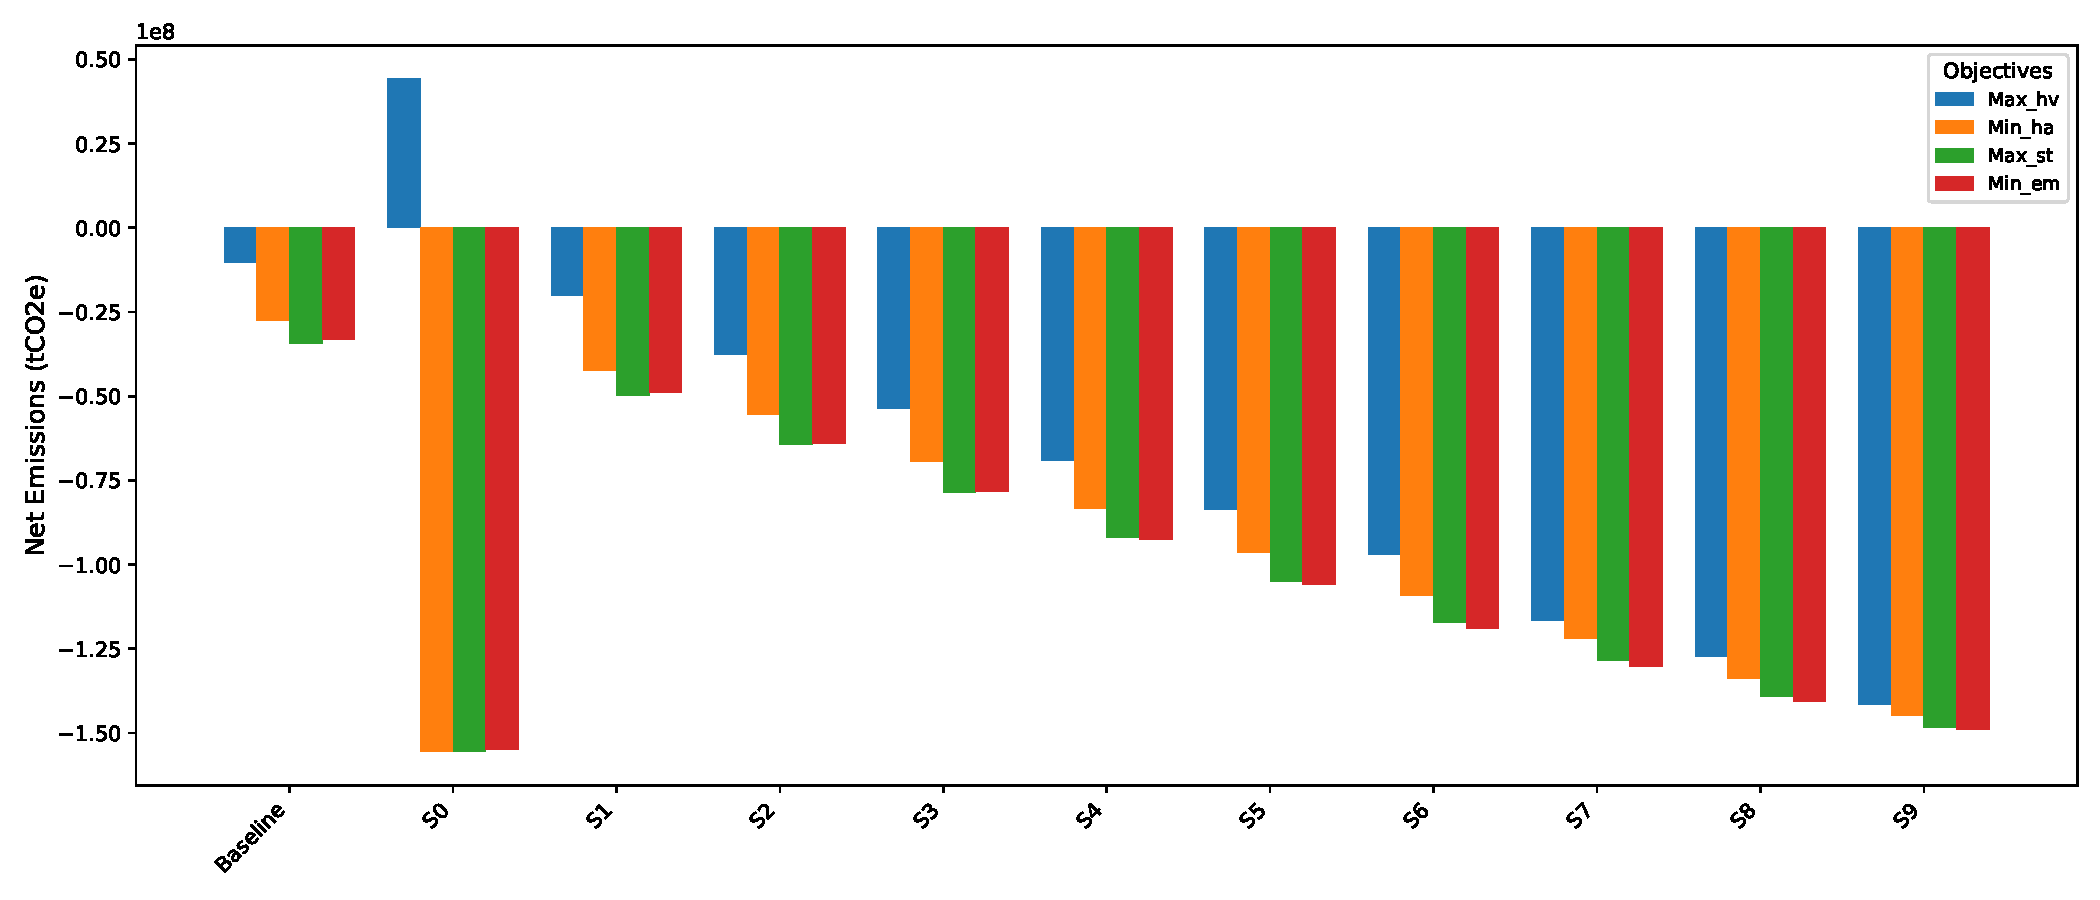
\includegraphics[width=\linewidth]{Fig.7.pdf} 
    \caption{Comparison of net emissions across different scenarios and planning objectives in the forest lands surrounding Mining site 1.}
    \label{fig:Fig.7}    
\end{figure}

\begin{figure}[H]
    \centering
    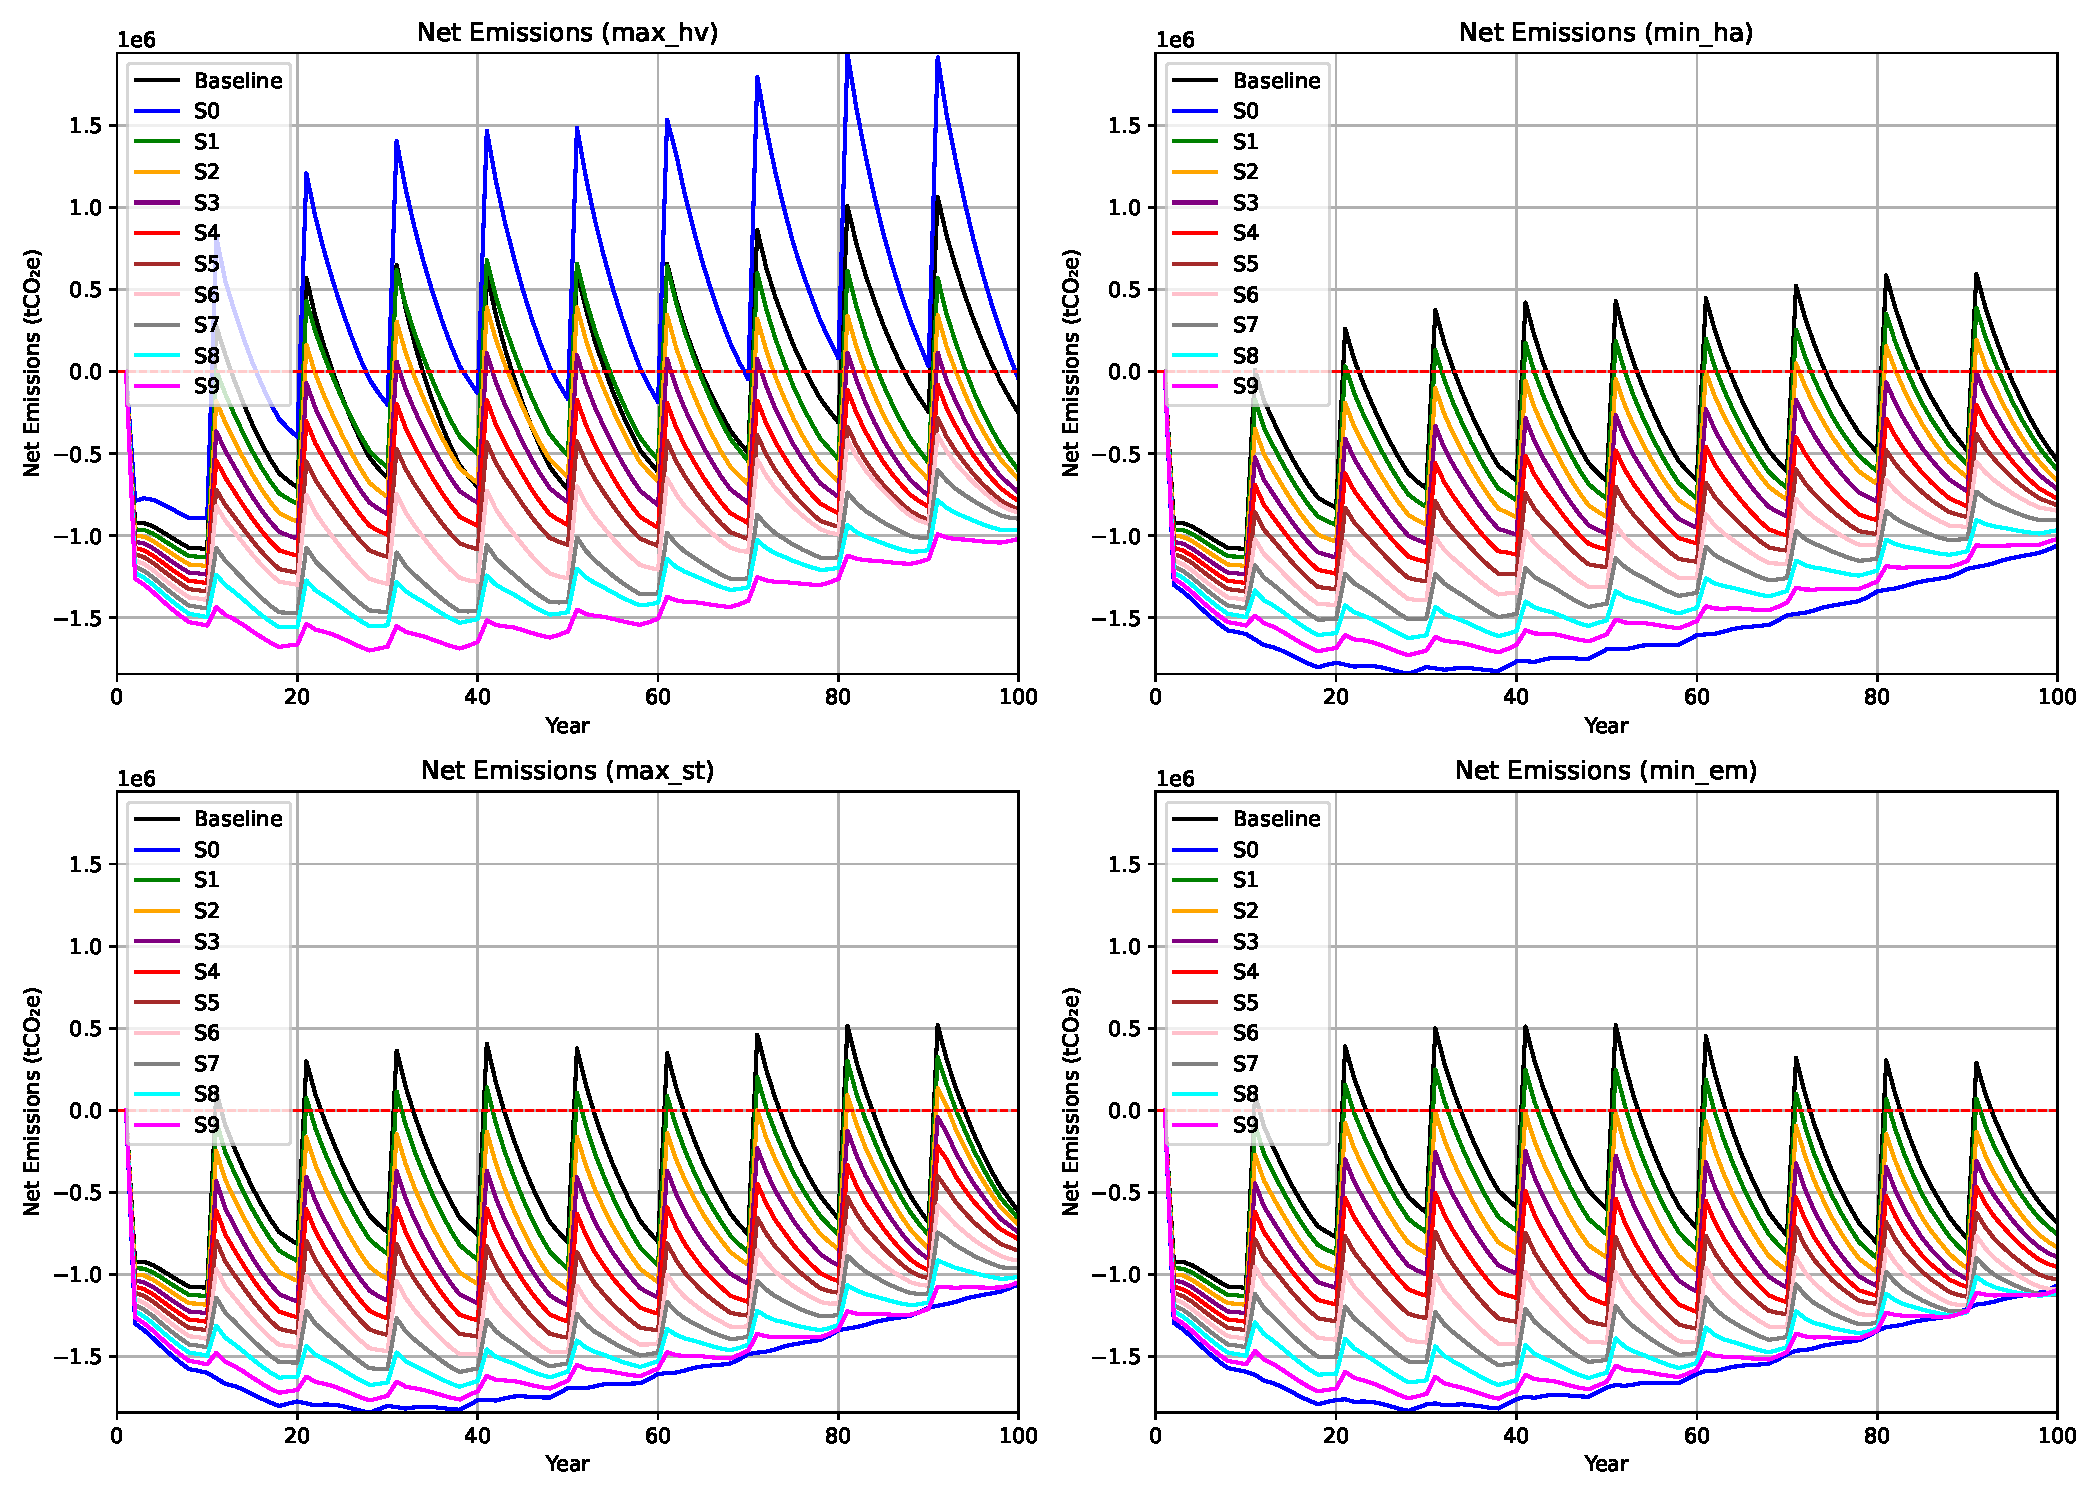
\includegraphics[width=\linewidth]{Fig.8.pdf} 
    \caption{Comparison of net emissions across different scenarios and planning objectives in the forest lands surrounding Mining Site 1 over a 100-year planning horizon.}
    \label{fig:Fig.8}    
\end{figure}
Figure \ref{fig:Fig.9} presents a comparative analysis of old growth forest area across harvesting scenarios and planning objectives in the forest lands surrounding Mining Site 1. The results indicate a general increase in the old growth area from Scenario S0 through S9 under all objectives. Notably, scenarios under minimizing harvested area and maximizing ecosystem carbon stocks tend to preserve more old growth area than the maximizing harvested volume objective and minimizing net carbon emissions. However, the difference in old growth preservation decreases as the harvest intensity decreases from Scenario S1 to Scenario S9. The smallest old growth area is observed in Scenario S0, which focuses on maximizing harvest levels.

Figure \ref{fig:Fig.10} presents a comparison of tree species diversity across various harvesting scenarios and planning objectives in the forest lands surrounding Mining Site 1. The values range from 0.7 to 0.77, indicating moderately high tree species diversity under all scenarios and objectives. Notably, there is no dramatic decline in diversity under any specific scenario or objective. Among the planning objectives, minimizing net emissions consistently results in the lowest diversity values. Overall, the differences in species diversity are more strongly influenced by the planning objectives than by the specific harvesting scenarios.

\begin{figure}[H]
    \centering
    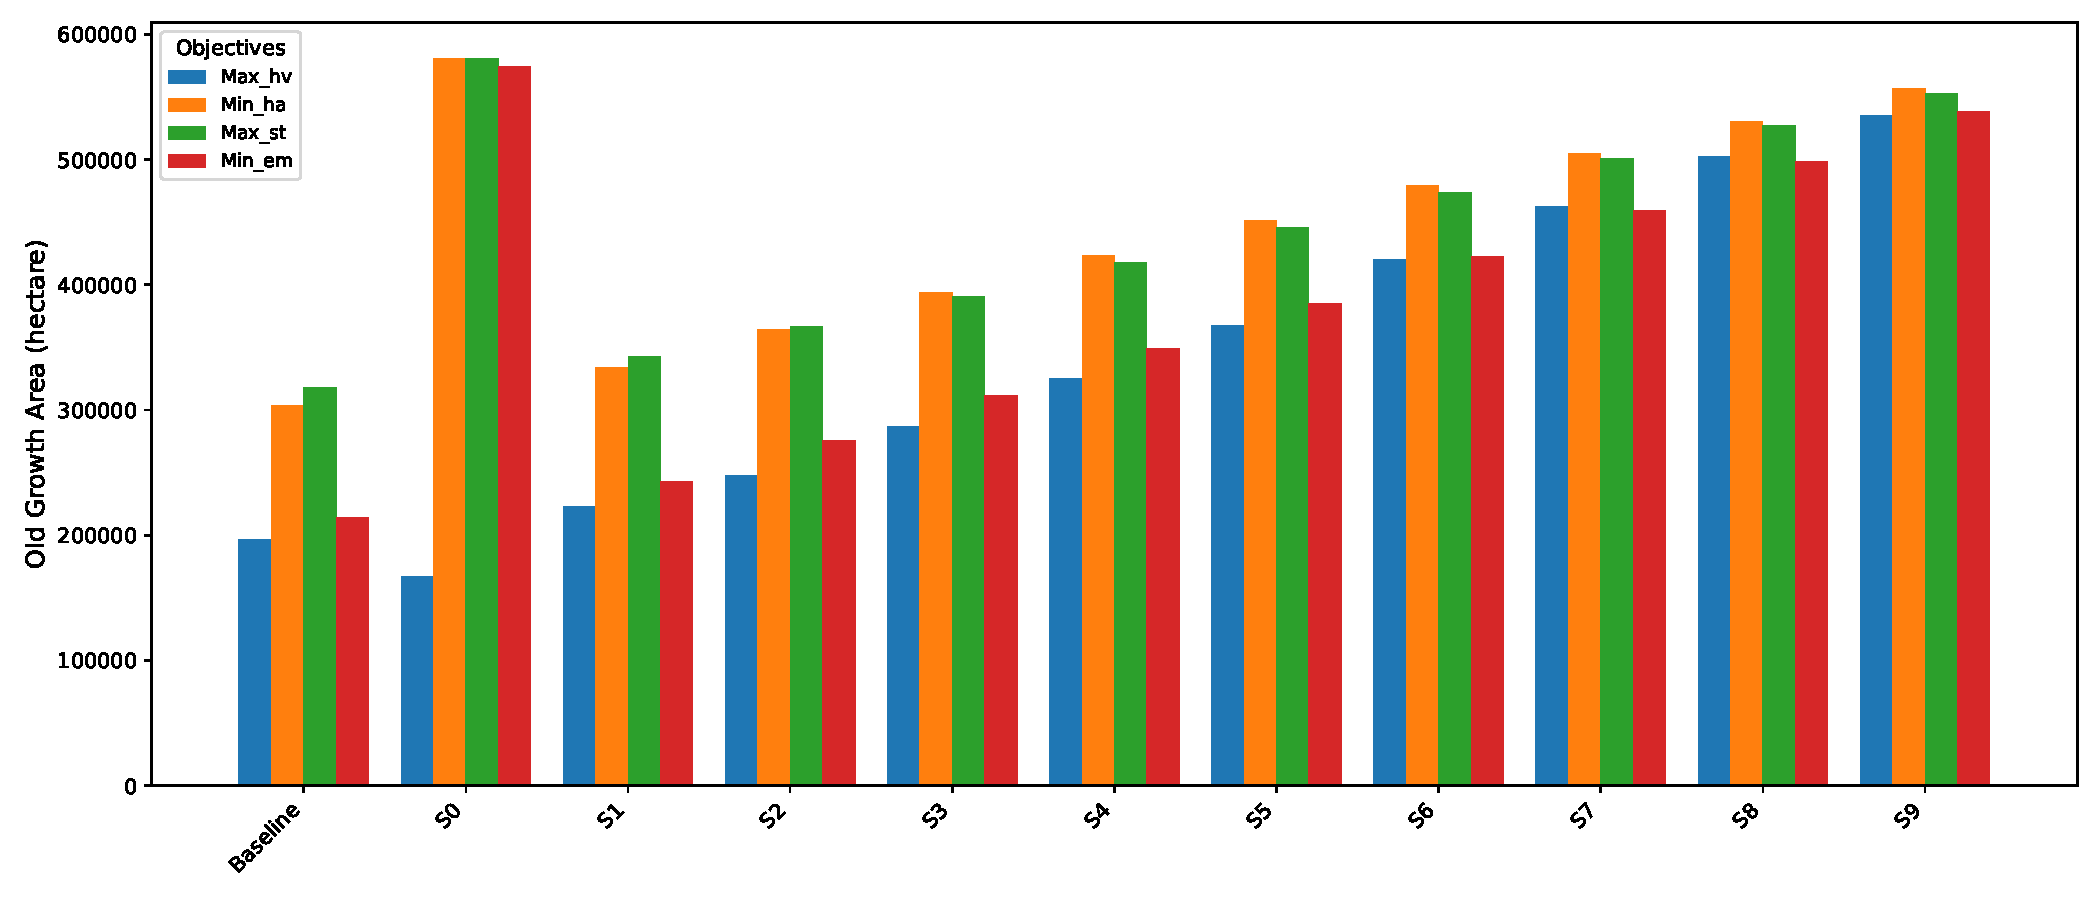
\includegraphics[width=\linewidth]{Fig.9.pdf} 
    \caption{Comparison of old growth attributes across harvesting scenarios and planning objectives in the forest lands surrounding Mining Site 1.}
    \label{fig:Fig.9}    
\end{figure}
\begin{figure}[H]
    \centering
    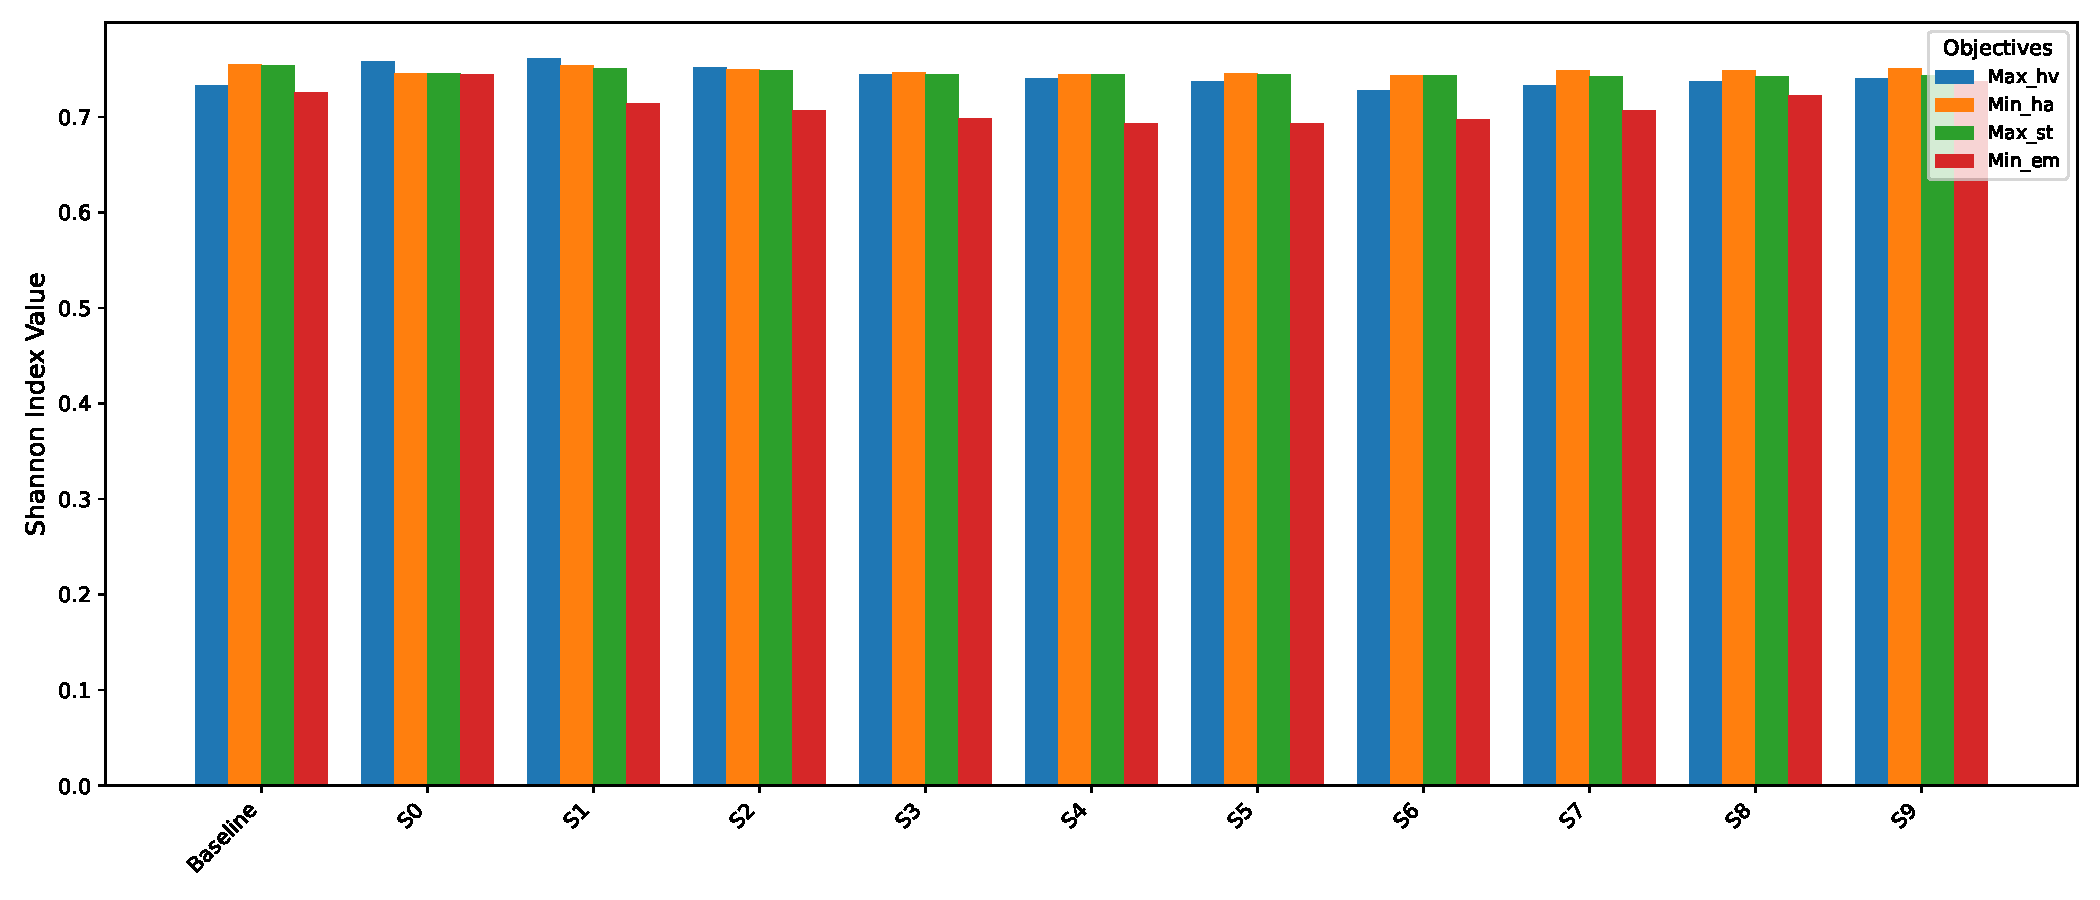
\includegraphics[width=\linewidth]{Fig.10.pdf} 
    \caption{Comparison of tree species diversity across harvesting scenarios and planning objectives in the forest lands surrounding Mining Site 1.}
    \label{fig:Fig.10}    
\end{figure}

\section{Discussion}
\label{sec: discussion}
\subsection{Impact of forest management objectives and harvest  intensity scenarios on key environmental indicators}
\label{sec: Impact of forest management objectives and harvest  intensity scenarios on key environmental indicator}

The aim of this study was to develop a prototype decision support framework for evaluating forest management objectives and harvest scenarios in relation to environmental indicators, and to assess how these decisions can contribute to mining sector decarbonization efforts. We examined a set of management objectives, including maximizing ecosystem carbon stocks or harvested volume and minimizing net carbon emissions or harvested area, in combination with a range of harvest intensity scenarios (S0–S9), applied across three case study sites. Environmental indicators included net emissions, old-growth forest area, and tree species diversity. Although we do not prescribe specific forest management strategies or generalize the findings to other forests and cases, the results offer insights based on the findings presented here. 

Our findings show that, under the same harvest-intensity level, different management objectives led to varying impacts on forest outcomes, including harvested volume and area, as well as growing stock. However, it is important to note that the objectives of minimizing harvested area, minimizing net carbon emissions, and maximizing ecosystem carbon stocks produced similar results. This pattern was consistent across all three case-study sites (see the baseline scenarios in Figures \ref{fig:Fig.3}, \ref{fig:Fig.A.1}, and \ref{fig:Fig.B.1} for mining sites 1, 2, and 3, respectively). 

As anticipated, variations in harvest intensity also led to corresponding shifts in environmental indicators. This finding is consistent with earlier work, such as that of \citet{Valipour2021}, which demonstrated how varying harvesting intensities can influence long-term forest dynamics and sustainability. Scenarios with reduced harvested volumes generally produce lower net emissions and increase the area of old-growth forest. However, while the harvest-intensity level changes linearly across scenarios, this does not hold true for environmental indicators. For mining site 1, under the objective of maximizing harvested volume (Table \ref{tab:KPIs_max_hv}), reducing the maximum harvest level from 90\% of the baseline harvested volume in scenario S1 to 80\% in scenario S2 (i.e. 9.5 million tonnes) results in an 87\% improvement in net emissions (almost 10 MtCO\textsubscript{2}e). Similar trends are evident across other management objectives and case-study sites. 

These differences become even more pronounced when comparing outcomes within the same harvest-intensity level scenario but across different management objectives. This finding is consistent with \citet{Makela2023}, who showed that forest management methods as well as harvest intensities influence wood production, carbon sequestration, and biodiversity. For instance, by shifting the forest management objective from maximizing harvested volume to minimizing net emissions, under the same baseline scenario in Mining Site 1, the net emissions improve from -10.2  MtCO\textsubscript{2}e to -34.3  MtCO\textsubscript{2}e (see Tables \ref{tab:KPIs_max_hv} and \ref{tab:KPIs_min_em}). Similarly, under the same baseline scenario, prioritizing the objective of maximizing carbon stock rather than maximizing harvested volume results in a 61\% increase in the old-growth index (see Tables \ref{tab:KPIs_max_hv} and \ref{tab:KPIs_max_st}).

The prototype developed in this study also provides a useful tool for monitoring changes in old-growth forests and tree species composition under different forest management objectives and harvest-intensity level scenarios. Although climate change mitigation and biodiversity conservation have both received increasing attention in recent years, they are often treated as separate priorities. In practice, these goals are rarely addressed in an integrated or coordinated manner \citep{Diaz2009}.
As highlighted by \citet{ezquerro2016operational}, forest management objectives have evolved significantly over the past few decades, with growing recognition of the importance of non-market ecosystem services such as biodiversity. However, effectively incorporating biodiversity considerations into forest planning remains a persistent challenge for both researchers and practitioners.

While the three case studies presented here are not intended to represent all forest types or regions, the results offer valuable insights into how biodiversity responds to different management strategies. The prototype’s outputs reveal that tree species composition can vary considerably depending on whether harvesting is excluded or allowed under various management goals. The baseline scenarios for Mining Sites 1, 2, and 3 (Figures \ref{fig:Fig.4}, \ref{fig:Fig.A.2}, and \ref{fig:Fig.B.2}) demonstrate how different strategies influence which species are retained. For example, in the baseline scenarios for forest lands surrounding Mining Sites 1, 2, and 3, Pines, Balsam, and Spruce are the dominant retained species under minimizing net carbon emissions objective. In contrast, Balsam becomes increasingly dominant under maximizing ecosystem carbon stocks objective across all sites. This shift suggests that species selection varies with management goals, reflecting differences in their relative capacity for carbon storage, based off the species different growth patterns and speed.

The findings also suggest that the choice of management objective has a greater impact on tree species diversity than the intensity of harvesting itself (Figures \ref{fig:Fig.10}, \ref{fig:Fig.A.8}, and \ref{fig:Fig.B.8}). In other words, it is not just how much harvesting takes place, but the broader goals guiding SFM that shape which species are retained. Similarly, \citet{Makela2023} showed that while harvest intensity strongly determines forest carbon stocks and fluxes, biodiversity responses are more strongly influenced by management practices than by harvesting levels and are relatively independent of carbon outcomes. Based on our results, overall species diversity does not change dramatically across scenarios, however small shifts in which species dominate can still affect how forests develop over time, including their structure, ecological succession, and resilience. Previous studies have noted that structurally complex forests often store more carbon \citep{Thom2019}, suggesting that species diversity may be an increasingly useful indicator for understanding carbon-related outcomes. 

The results also show that, in addition to species diversity, the old-growth forest area varies depending on the management objective. For climate-related objectives, the area of old-growth forest tends to be slightly larger under the carbon stock maximization objective than under the net carbon emissions minimization objective. This pattern is consistent across all three case study sites (see Tables \ref{tab:KPIs_max_hv}–\ref{tab:KPIs_min_ha}, \ref{tab:KPIs_max_hv_site2}–\ref{tab:KPIs_min_ha_site2}, and \ref{tab:KPIs_max_hv_site3}–\ref{tab:KPIs_min_ha_site3} for Mining Sites 1, 2, and 3, respectively). In line with findings from \citet{McGarvey2015}, this study adds to the growing body of evidence suggesting that old-growth forests managed for carbon storage can also serve as important reservoirs of biodiversity. 

\subsection{Evaluating the economic trade-offs of forest management scenarios for the mining sector}
\label{sec: Evaluating the Economic Trade-offs of Forest Management Scenarios for the Mining Sector}


Effective forest management as a climate mitigation strategy involves navigating various trade-offs, requiring a balance between long-term environmental and economic considerations \citep{Waring2020}. Although this study focuses on environmental indicators, revenue from harvested wood can also be calculated as an economic indicator, quantifying the financial returns derived from forest harvesting. However, relying solely on this measure provides only a partial representation of economic outcomes, as it does not capture broader costs, trade-offs, and value-chain effects. Nevertheless, it can serve as a useful baseline indicator for preliminary economic assessment.

According to the 2021 Economic Start of BC's Forest Sector report published by \citet{BC_ForestSector_2021}, timber harvests in BC totaled 52.7 million $m^3$ in 2021 and generated \$1.9 billion in provincial government revenues, which corresponds to an average revenue of approximately \$36 per cubic meter. In this study, for instance, in the mining site 1 under maximizing harvested volume (Table \ref{tab:KPIs_max_hv}), moving from the baseline scenario (harvested volume of 95.4 million m$^3$ and net emissions of -10.2 Mt CO$_2$e) to Scenario S1 (harvesed volume of 85.8 million m$^3$ and net emissions of -20.2 Mt CO$_2$e) reduces the harvested volume by 10\% results in a reduction of 10 Mt CO$_2$e. Considering an average revenue of approximately \$36 per cubic meter, the reduction in harvested volume (9.6 million m$^3$) corresponds to a foregone revenue of roughly \$345.6 million. Consequently, the implied carbon price (i.e., the opportunity cost of emission reduction measured as foregone revenue per 
additional tonne of CO$_2$e mitigated) associated with this harvest reduction is estimated as

\[
\text{Implied carbon price} = \frac{\text{Revenue loss}}{\text{Emission reduction}} \approx \frac{345.6 \text{ million \$}}{10 \text{ Mt CO$_2$e}} \approx 34.6~\text{\$/tCO$_2$e}.
\]

\begin{table}[htbp]
\centering
\caption{Implied carbon price (\$/tCO$_2$e) across scenarios and management objective.}
\label{tab:implied_carbon_price_objectives}
\begin{tabular}{lllll}
\toprule
Scenario & Max\_hv & Min\_ha & Max\_cs & Min\_em \\
\midrule
S1 & 34.6 & 20.2 & 19.4 & 19.2 \\
S2 & 25.0 & 21.5 & 20.1 & 19.6 \\
S3 & 23.8 & 21.6 & 20.4 & 19.9 \\
S4 & 23.4 & 21.5 & 20.8 & 20.2 \\
S5 & 23.4 & 21.7 & 21.2 & 20.6 \\
S6 & 23.8 & 22.1 & 21.7 & 21.0 \\
S7 & 22.7 & 23.3 & 23.3 & 22.6 \\
S8 & 23.5 & 23.5 & 23.9 & 23.3 \\
S9 & 23.6 & 23.9 & 24.5 & 24.2 \\
\bottomrule
\end{tabular}

\vspace{2mm}
\footnotesize\emph{Notes:} Values represent the magnitude of 
$\Delta \text{Revenue}/\Delta \text{Emissions}$, calculated relative to the 
baseline scenario within each management objective.
\end{table}



Table~\ref{tab:implied_carbon_price_objectives} reports the implied carbon price 
across alternative management objectives. 
Under the maximizing harvested volume objective, the implied price is highest in S1 
(34.6~\$/tCO$_2$e) and declines thereafter, stabilizing around 22--25~\$/tCO$_2$e 
for S2--S9. In contrast, the other objectives exhibit a narrower range of values and a gradual 
convergence toward approximately 23--24~\$/tCO$_2$e in the more stringent 
scenarios (S7--S9). This pattern suggests that once emission reductions become 
substantial, the marginal economic trade-off per additional tonne of CO$_2$e 
becomes relatively insensitive to the specific management objective. 

The estimated implied carbon prices (approximately 19--35~\$/tCO$_2$e across 
scenarios) fall well within the range of Canada's national carbon pricing 
framework. Canada's federal carbon pricing system introduced a minimum price 
of 65~\$/tCO$_2$e in 2023, increasing by 15~\$ annually to reach 
170~\$/tCO$_2$e by 2030 \citep{CanadaCarbonPricing2023}. In this context, the opportunity cost of emission reduction estimated in this study lies substantially below the projected 2030 benchmark price. Although the results are site-specific and not intended for broad generalization, they suggest that the mining industry could consider investing in harvest-based mitigation strategies as a cost-effective alternative to directly paying the prevailing carbon price.

Forest management decisions surrounding mining sites carry not only environmental consequences but also important economic implications. By comparing alternative management scenarios, such as reduced harvesting, we can assess both the foregone revenue from timber extraction and the potential financial gains associated with improved carbon outcomes. For instance, scenarios that limit harvesting may reduce direct economic returns from wood products, yet they can significantly enhance net carbon emissions reductions. When these emissions benefits are translated into monetary terms using prevailing carbon prices, they provide a tangible metric for evaluating whether the carbon value gained can offset, or even exceed, the economic losses from reduced timber revenues.

The developed prototype decision support framework in this study enables exploratory quantification of trade-offs, helping to identify thresholds at which environmental benefits may begin to conflict with economic viability in this case-study context. By comparing outcomes across a range of scenarios, the tool supports planners and decision-makers in evaluating forest management objectives and strategies. Consistent with the findings of \citet{Hiltunen2021}, the results indicate that no single management strategy simultaneously maximizes both environmental and economic performance. 

\subsection{Scope and limitations}
\label{sec: limitations}
To our knowledge, few case studies present a prototype decision support framework that tracks carbon from forests to HWPs and the resulting displacement effects. The prototype also incorporates various objectives, scenarios, and constraints to simulate and optimize forest management practices. While the prototype is designed to be adaptable across differing data and objectives, the results presented are specific to the defined case studies and may not be directly applicable to other contexts.

Despite the benefits, this study has some limitations that present opportunities for future research. We assumed that the harvested wood is converted into only two types of HWPs, i.e., lumber and paper. Also, a simplified half-life of 30 years was assumed for lumber. A more rigorous life-cycle assessment could refine the results. In addition, while the defined scenarios were based on the percentage of maximum harvested volume, considering other constraints can result in more realistic scenarios.

The main goal of this study was to demonstrate the functionality of the prototype framework to generate results for each scenario. However, a sensitivity analysis is not conducted. Such analysis helps decision makers to know how sensitive the results would be against changes in input parameters such as half-lives and displacement factors. 

The key performance indicators employed in this study were primarily limited to environmental dimensions. Although we examined the trade-off between reduced direct revenues from harvested wood products and associated emissions resulting from lower harvest levels,  specifically to assess whether harvest-level management could be considered a NbS for supporting the mining sector’s efforts to achieve net-zero emissions by 2050, these metrics do not capture broader dimensions of social sustainability, such as community well-being, equity, or long-term economic resilience. Similarly, the biodiversity indicators focused primarily on tree species diversity and old-growth forest area, without accounting for other critical components of forest ecosystems, such as wildlife habitats, understory vegetation, or soil biodiversity. These simplifications, while necessary for tractability, point to opportunities for future work to incorporate a more holistic set of indicators that better reflect the complexity of forest socio-ecological systems. Furthermore, each of these aspects can be considered as objective functions along with harvested area and volume, carbon stocks, and carbon emissions in a multi-objective optimization model. This approach can enable decision makers to explore potential trade-offs between these objectives. 

Finally, we modeled only clear-cutting in the prototype framework. Including other forest management activities, such as selective cutting, planting, fertilizing, and/or partial cutting, would provide a more complete assessment of their impacts on environmental and socioeconomic outcomes.

\section{Conclusion}
\label{sec: conclusion}
This study developed and applied a prototype open-source decision support framework to evaluate forest management strategies as an NbS for decarbonization in the context of mining operations in BC, Canada. By integrating environmental indicators, the prototype enables an initial assessment of trade-offs among various forest management objectives and harvesting scenarios.

The results indicate that although harvest levels vary linearly across scenarios, environmental indicators, such as net emissions, old-growth retention, and species diversity, respond in more complex and nonlinear ways. Management objectives play a decisive role in shaping these outcomes, often exerting a stronger influence than harvest amount alone. According to the results, scenarios focused on maximizing ecosystem carbon stocks or minimizing net carbon emissions achieved notable environmental benefits. This analysis underscores the importance of clearly defined planning objectives in SFM. 

The findings indicate that forest management near mining sites can offer a measurable and economically interpretable mitigation pathway. By quantifying the trade-off between foregone timber revenues and emission reductions, the study derives an implied carbon price comparable to Canada’s carbon pricing benchmarks. Nevertheless, site-specific conditions and broader socioeconomic factors should be carefully considered when applying these insights.

While the findings provide valuable insights, they are based on a limited set of case studies and should not be generalized across all forest ecosystems or management contexts. The modeling relies on a number of assumptions regarding species responses, decay rates, and displacement effects, which may vary in other geographic or institutional settings. Future work should expand the application of the prototype framework across different forest types and policy contexts and incorporate dynamic ecological feedback and more nuanced socioeconomic indicators. Despite these limitations, the study offers a practical and adaptable tool for exploring forest management strategies as nature-based decarbonization solutions and contributes to a growing body of work at the intersection of forest management, climate action, and sustainable development.

While the prototype facilitates the assessment of different forest management scenarios and KPIs, this study only focused on harvest scheduling and a limited set of KPIs, so it does not cover the full range of ecological and socioeconomic factors. The system also does not include other forest management practices, such as selective cutting, planting, or fertilization strategies, which could have a big impact on carbon storage and biodiversity. Adding these practices to the prototype would provide a more complete picture of how forest management affects carbon neutrality.


\section*{CRediT authorship contribution statement}
\label{sec: CRediT}
\textbf{Elaheh Ghasemi}: Conceptualization, Data curation, Formal analysis, Methodology, Software, Validation, Visualization, Writing – original draft. \textbf{Kathleen Coupland}: Data curation, Formal analysis, Writing – review \& editing. \textbf{Salar Ghotb}: Software, Writing – original draft. \textbf{Gregory Paradis}: Data curation, Formal analysis, Funding acquisition, Methodology, Project administration, Resources, Software, Writing – review \& editing, Supervision.

\section*{Declaration of competing interest}
\label{sec:Declaration of Competing Interest}
The authors declare that they have no known competing financial interests or personal relationships that could have appeared to influence the work reported in this article.

\section*{Use of AI and AI-assisted technologies in scientific writing}
In the final stage of manuscript preparation, the authors used a generative AI tool to assist with language polishing and to verify that the submission package conformed to the journal's Guide for Authors (e.g., highlights length/format and presence of required declarations). No scientific analysis, results generation, or novel content creation was performed by AI. The authors take full responsibility for the content of this work.

\section*{Funding}
This work was supported by Mitacs through the Accelerate Program in partnership with Newmont Goldcorp Inc. (grant IT32088), by the World Economic Forum through the Hoffmann Fellowship program (grant AWD-028246), and by the Bradshaw Research Initiative in Minerals and Mining (BRIMM).

\section*{Acknowledgments}
\label{sec:acknowledgments}
We thank Yunhao Xu and Rosalia Jaffray for their contributions to writing and reviewing early drafts of this manuscript.


\section*{Data availability and reproducibility}
\label{sec: data availability}
The data and code supporting the findings of this study are available in \citet{nbds_dss_2025}. The latest prototype framework and example notebooks are hosted at \url{https://github.com/UBC-FRESH/nbds_dss}.

\bibliographystyle{elsarticle-num-names}
\bibliography{references}

\appendix

\newpage
% Avoid duplicate hyperref anchors for figures when counters reset in appendices
\makeatletter
\renewcommand\theHfigure{\thesection.\arabic{figure}}
\renewcommand\theHtable{\thesection.\arabic{table}}
\makeatother
\phantom{}
\section{Parameter values}
\label{sec:appendix1}
\renewcommand{\thetable}{A.\arabic{table}}
\setcounter{table}{0}
\setcounter{figure}{0}
In this appendix, the values for model parameters are listed.

\begin{table}[H]
\centering
\caption{Values of the input parameters of the model.}
\label{tab:parameters}
\begin{adjustbox}{width=\textwidth}
{\small
\begin{tabular}{llc}
\toprule
\makecell[l]{Parameter} & 
\makecell[l]{Description} & 
\makecell[c]{Value} \\
\midrule
$\beta_j$ & Admissible level of variation on yield of targeted output & 0.05 \\
$w$ & Wood density & 460 $kg/m^{3}$ \\
$n$ & Carbon content & 0.5\\
$P$ & Set of HWPs & Solid wood, Paper\\
$t_{1/2}^{p}$ & half life of HWP p & Solid wood: 30, Paper: 2\\
$D$ & Set of products replaced by HWPs & Concrete\\
$f$ & Displacement factor & 1\\
$r_{pd}$ & percentage of HWP p that would replace product d & Solid wood: 0.4, Paper: 0\\
$m_{p}$ & percentage of harvest amount converted to HWP p & Solid wood: 0.8, Paper: 0.2\\
\bottomrule
\end{tabular}
}
\end{adjustbox}
\end{table}


\section{Results of Mining Site 2}
\label{sec:appendix2}
\renewcommand{\thetable}{A.\arabic{table}}
\setcounter{table}{0}
\setcounter{figure}{0}
Here, we present the detailed results from running all defined scenarios under various objectives for Mining Site 2.

\begin{figure}[H]
    \centering
    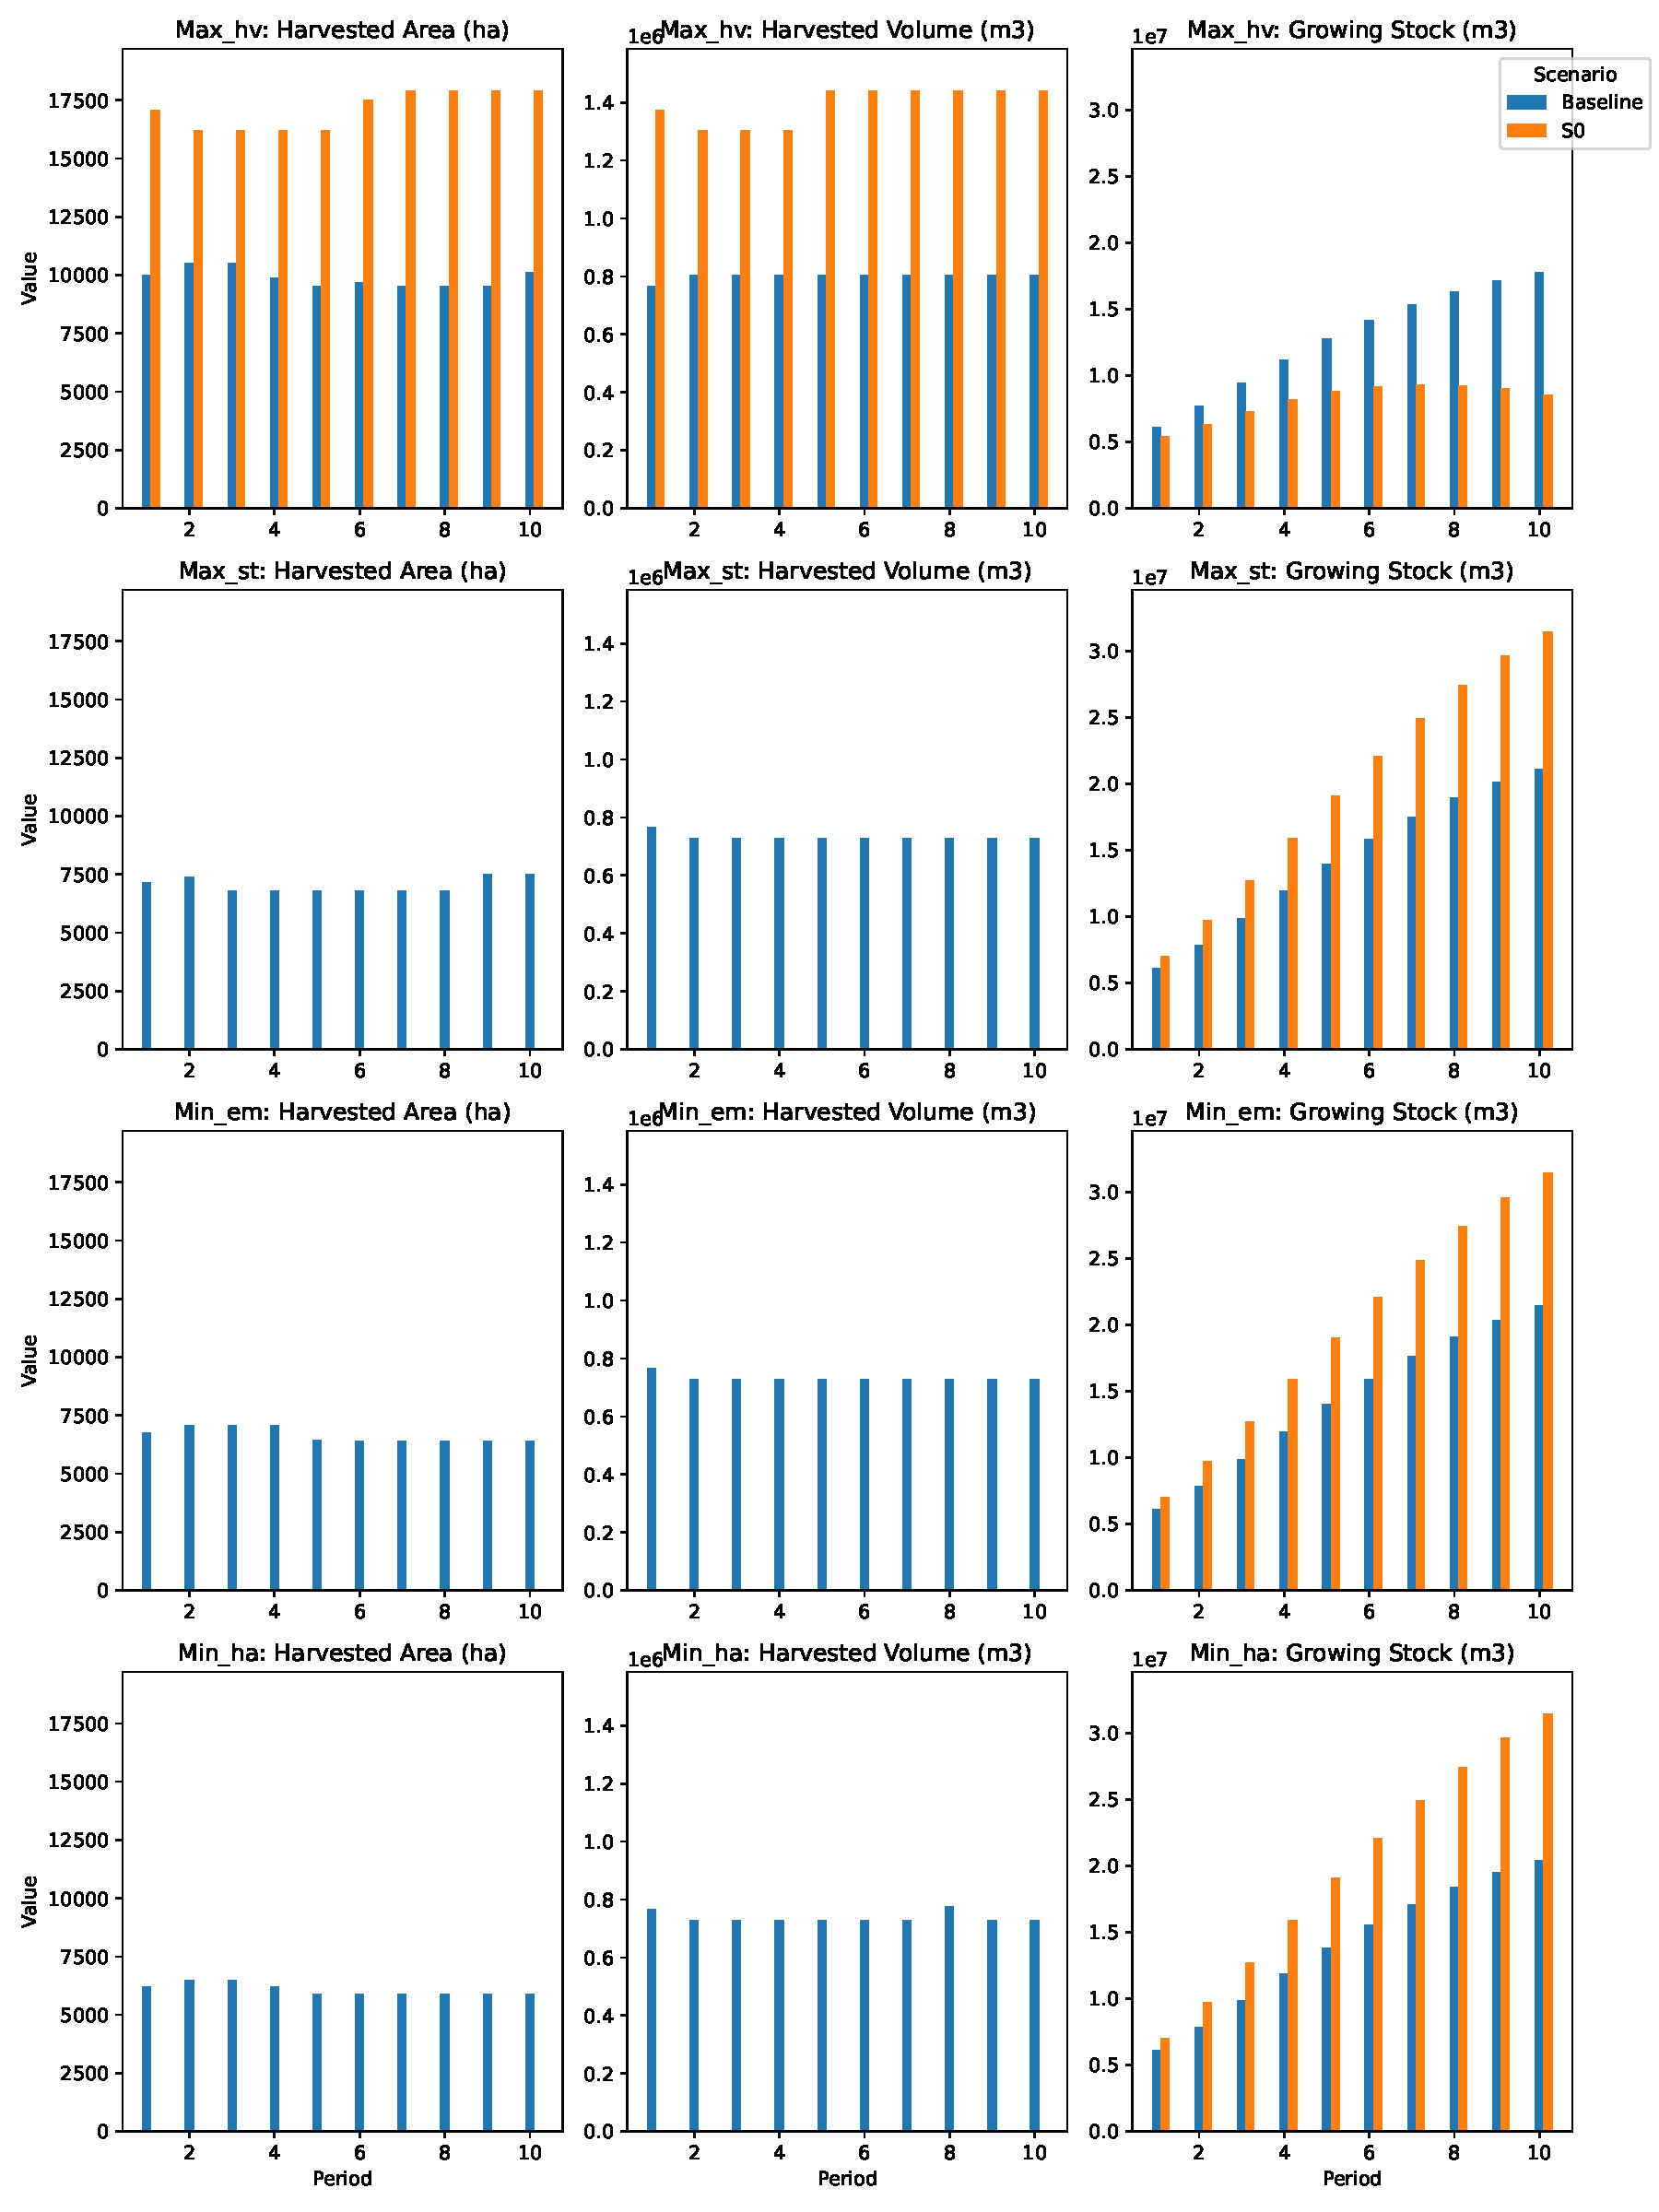
\includegraphics[width=\linewidth]{Fig.A.1.pdf} 
    \caption{Comparison of harvested area, volume, and growing stock in the forest lands surrounding Mining Site 2: Baseline vs. scenario S0 across planning objectives.}
    \label{fig:Fig.A.1}    
\end{figure}

\begin{figure}[H]
    \centering
    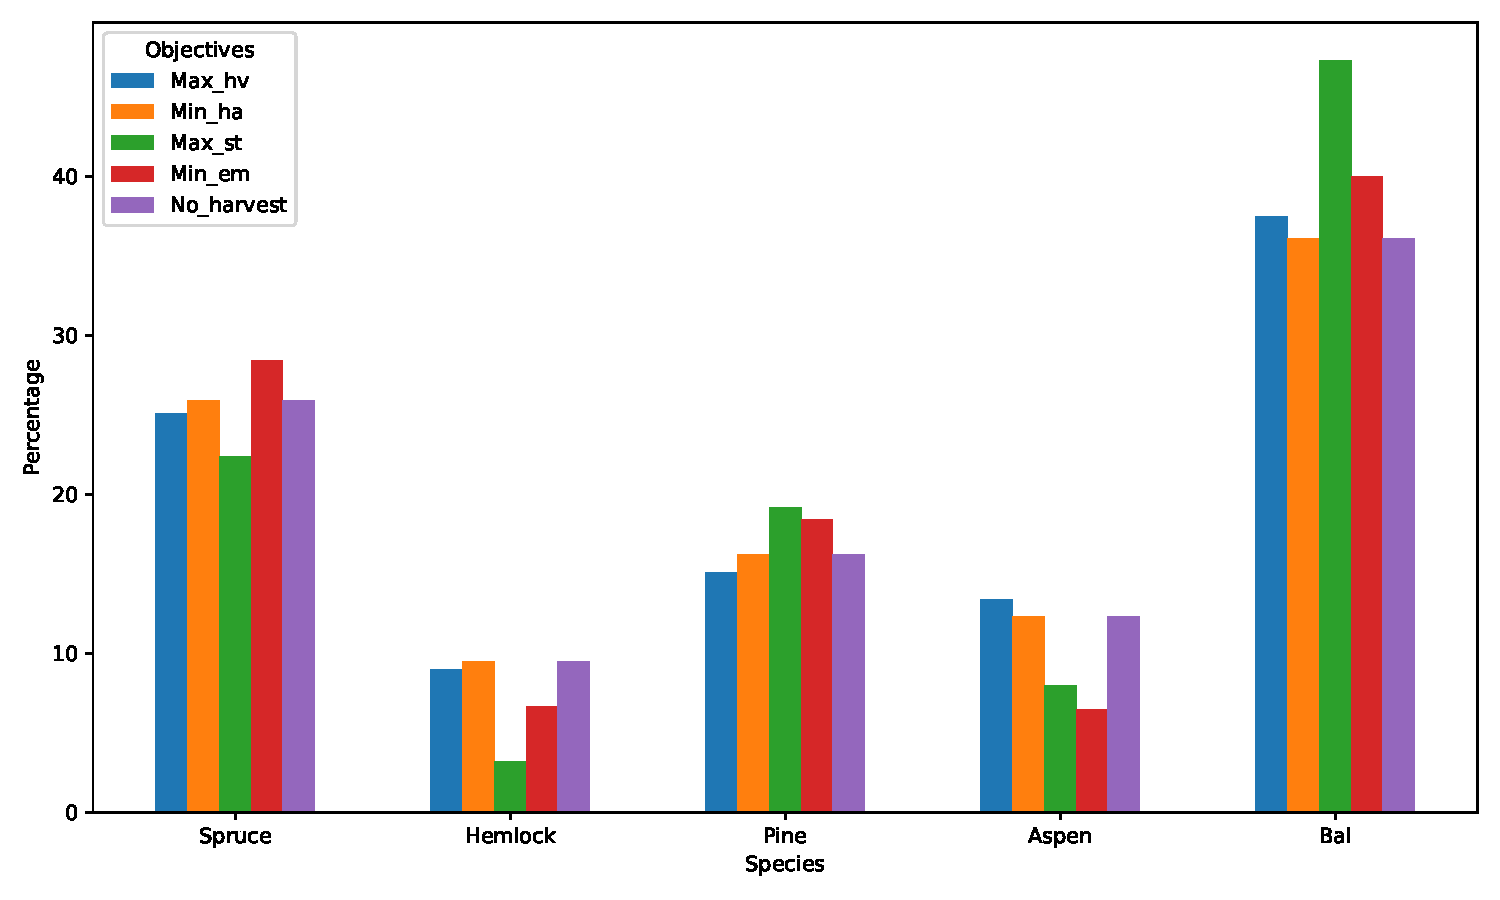
\includegraphics[width=\linewidth]{Fig.A.2.pdf} 
    \caption{Comparison of retained tree species under planning objectives and the no-harvest condition in forest lands surrounding Mining Site 2 (baseline scenario).}
    \label{fig:Fig.A.2}    
\end{figure}

\begin{table}[H]
\centering
\caption{Comparison of KPIs across harvesting scenarios for the forest lands surrounding Mining Site 2 under the objective of maximizing harvested volume.}
\label{tab:KPIs_max_hv_site2}
\begin{adjustbox}{width=\textwidth}
{\small
\begin{tabular}{lrrrr}
\toprule
\makecell[l]{Scenario} & 
\makecell[r]{Harvest\\Volume\\(Mm\textsuperscript{3})} & 
\makecell[r]{Net\\Emissions\\(MtCO\textsubscript{2}e)} & 
\makecell[r]{Species\\Indicator} & 
\makecell[r]{Old Growth\\(k ha)} \\
\midrule
Baseline &  8.01  & -22.43 &  0.923 & 26.6  \\
S0       & 13.93  &  -6.21 & 0.809 & 14.7  \\
S1       &  7.20  & -20.82 &  0.917 & 31.5  \\
S2       &  6.40  & -24.44 &  0.920 & 33.4  \\
S3       &  5.60  & -27.88 &  0.918 & 34.9  \\
S4       &  4.80  & -30.83 &  0.916 & 36.6  \\
S5       &  4.00  & -33.80 &  0.917 & 39.0  \\
S6       &  3.20  & -37.20 &  0.917 & 40.7  \\
S7       &  2.40  & -40.17 &  0.920 & 42.7  \\
S8       &  1.60  & -43.34 &  0.922 & 44.9  \\
S9       &  0.80  & -46.26 &  0.926 & 52.3  \\
\bottomrule
\end{tabular}
}
\end{adjustbox}
\end{table}


\begin{table}[H]
\centering
\large
\caption{Comparison of KPIs across harvesting scenarios for the forest lands surrounding Mining Site 2 under the objective of maximizing carbon stock.}
\label{tab:KPIs_max_CS_site2}
\begin{adjustbox}{width=\textwidth}
{\small
\begin{tabular}{lrrrrrr} % first column left aligned
\toprule
\makecell[l]{Scenario} & 
\makecell[r]{Harvest\\Volume\\($\mathrm{Mm}^3$)} &
\makecell[r]{Carbon\\Stock\\(MtC)} & 
\makecell[r]{Net\\Emissions\\(MtCO\textsubscript{2}e)} & 
\makecell[r]{Species\\Indicator} & 
\makecell[r]{Old Growth\\(k ha)} \\
\midrule
Baseline & 7.32 & 36.67 & -32.70 & 0.818 & 24.7 \\
S0       & -    & 39.68 & -49.43 & 0.929 & 48.8 \\
S1       & 6.58 & 37.10 & -35.00 & 0.822 & 26.3 \\
S2       & 5.85 & 37.50 & -37.14 & 0.828 & 28.3 \\
S3       & 5.12 & 37.88 & -39.16 & 0.849 & 30.2 \\
S4       & 4.39 & 38.23 & -41.09 & 0.864 & 32.2 \\
S5       & 3.66 & 38.56 & -42.92 & 0.869 & 34.4 \\
S6       & 2.93 & 38.87 & -44.60 & 0.878 & 36.7 \\
S7       & 2.19 & 39.13 & -46.23 & 0.896 & 39.0 \\
S8       & 1.46 & 39.36 & -47.54 & 0.909 & 42.0 \\
S9       & 0.74 & 39.54 & -48.58 & 0.921 & 45.5 \\
\bottomrule
\end{tabular}
}
\end{adjustbox}
\end{table}

\begin{table}[H]
\centering
\caption{Comparison of KPIs across harvesting scenarios for the forest lands surrounding Mining Site 2 under the objective of minimizing net emissions.}
\label{tab:KPIs_min_em_site2}
\begin{adjustbox}{width=\textwidth}
{\small
\begin{tabular}{lrrrrrr}
\toprule
\makecell[l]{Scenario} & 
\makecell[r]{Harvest\\Volume\\($\mathrm{Mm}^3$)} & 
\makecell[r]{Net\\Emissions\\(MtCO\textsubscript{2}e)} & 
\makecell[r]{Species\\Indicator} & 
\makecell[r]{Old Growth\\(k ha)} \\
\midrule
Baseline & 7.32 &-33.38 & 0.867 & 19.8 \\
S0       & 0.9  &-49.41 & 0.928 & 48.6 \\
S1       & 6.85 &-35.59 & 0.869 & 25.0 \\
S2       & 5.85 &-37.68 & 0.872 & 23.1 \\
S3       & 5.12 &-39.67 & 0.877 & 25.1 \\
S4       & 4.93 &-41.55 & 0.877 & 27.4 \\
S5       & 3.66 &-43.33 & 0.881 & 30.2 \\
S6       & 2.93 &-44.98 & 0.890 & 33.2 \\
S7       & 2.19 &-46.28 & 0.894 & 36.8 \\
S8       & 1.46 &-47.58 & 0.905 & 39.9 \\
S9       & 0.74 &-48.65 & 0.919 & 43.6 \\
\bottomrule
\end{tabular}
}
\end{adjustbox}
\end{table}

\begin{table}[H]
\centering
\caption{Comparison of KPIs across harvesting scenarios for the forest lands surrounding Mining Site 2 under the objective of minimizing harvested area.}
\label{tab:KPIs_min_ha_site2}
\begin{adjustbox}{width=\textwidth}
{\small
\begin{tabular}{lrrrrr}
\toprule
\makecell[l]{Scenario} & 
\makecell[r]{Harvest\\Volume\\($\mathrm{Mm}^3$)} &
\makecell[r]{Harvest\\Area\\(k ha)} & 
\makecell[r]{Net\\Emissions\\(MtCO\textsubscript{2}e)} & 
\makecell[r]{Species\\Indicator} & 
\makecell[r]{Old Growth\\(k ha)} \\
\midrule
Baseline & 7.32 & 60.74  & -30.67 & 0.893 & 27.3 \\
S0       & 0.02 & --     & -49.43 & 0.929 & 48.8 \\
S1       & 6.58 & 52.60  & -32.93 & 0.894 & 28.7 \\
S2       & 5.85 & 44.81  & -35.23 & 0.889 & 31.0 \\
S3       & 5.12 & 37.41  & -37.36 & 0.888 & 33.4 \\
S4       & 4.39 & 30.46  & -39.35 & 0.885 & 35.1 \\
S5       & 3.66 & 23.93  & -41.38 & 0.884 & 37.9 \\
S6       & 2.93 & 17.91  & -43.11 & 0.888 & 40.8 \\
S7       & 2.19 & 12.41  & -44.77 & 0.893 & 43.1 \\
S8       & 1.46 &7.48    & -46.46  & 0.899 & 45.5 \\
S9       & 0.74 & 3.19   & -48.02  & 0.914 & 47.2 \\
\bottomrule
\end{tabular}
}
\end{adjustbox}
\end{table}


\begin{figure}[H]
    \centering
    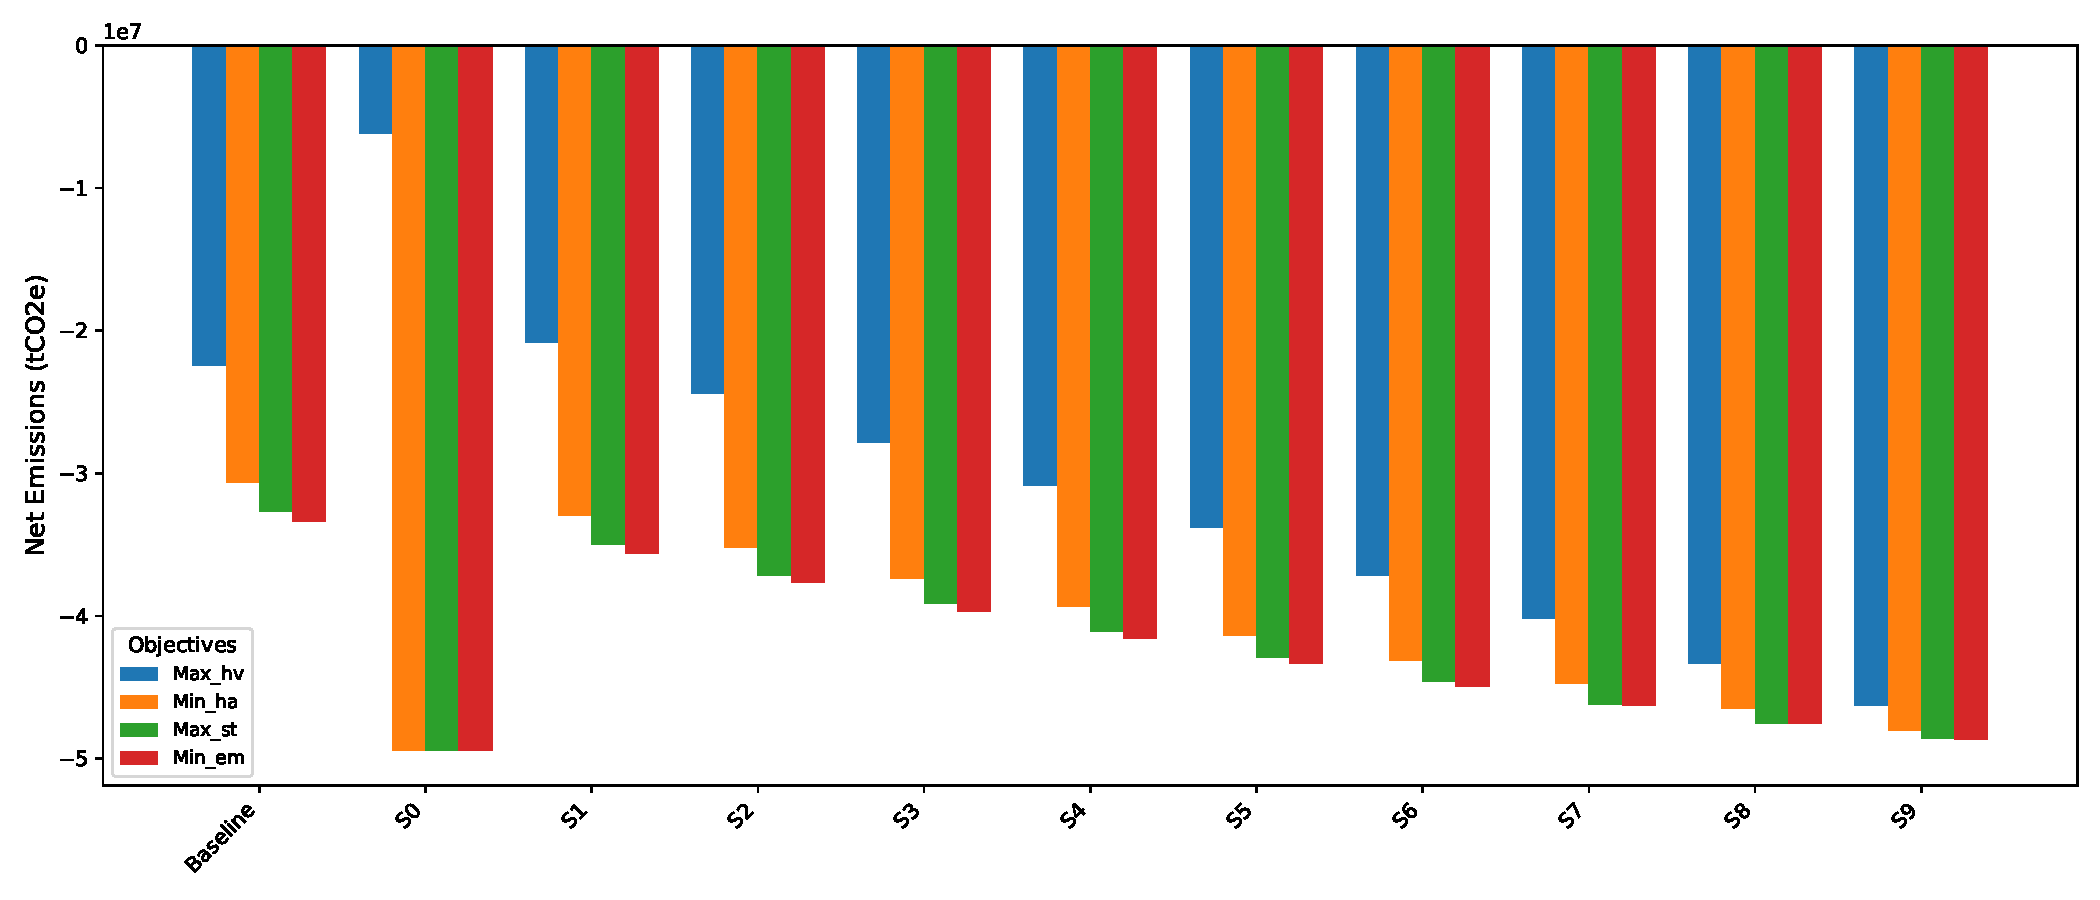
\includegraphics[width=\linewidth]{Fig.A.5.pdf} 
    \caption{Comparison of net emissions across different scenarios and planning objectives in the forest lands surrounding Mining site 2.}
    \label{fig:Fig.A.5}    
\end{figure}

\begin{figure}[H]
    \centering
    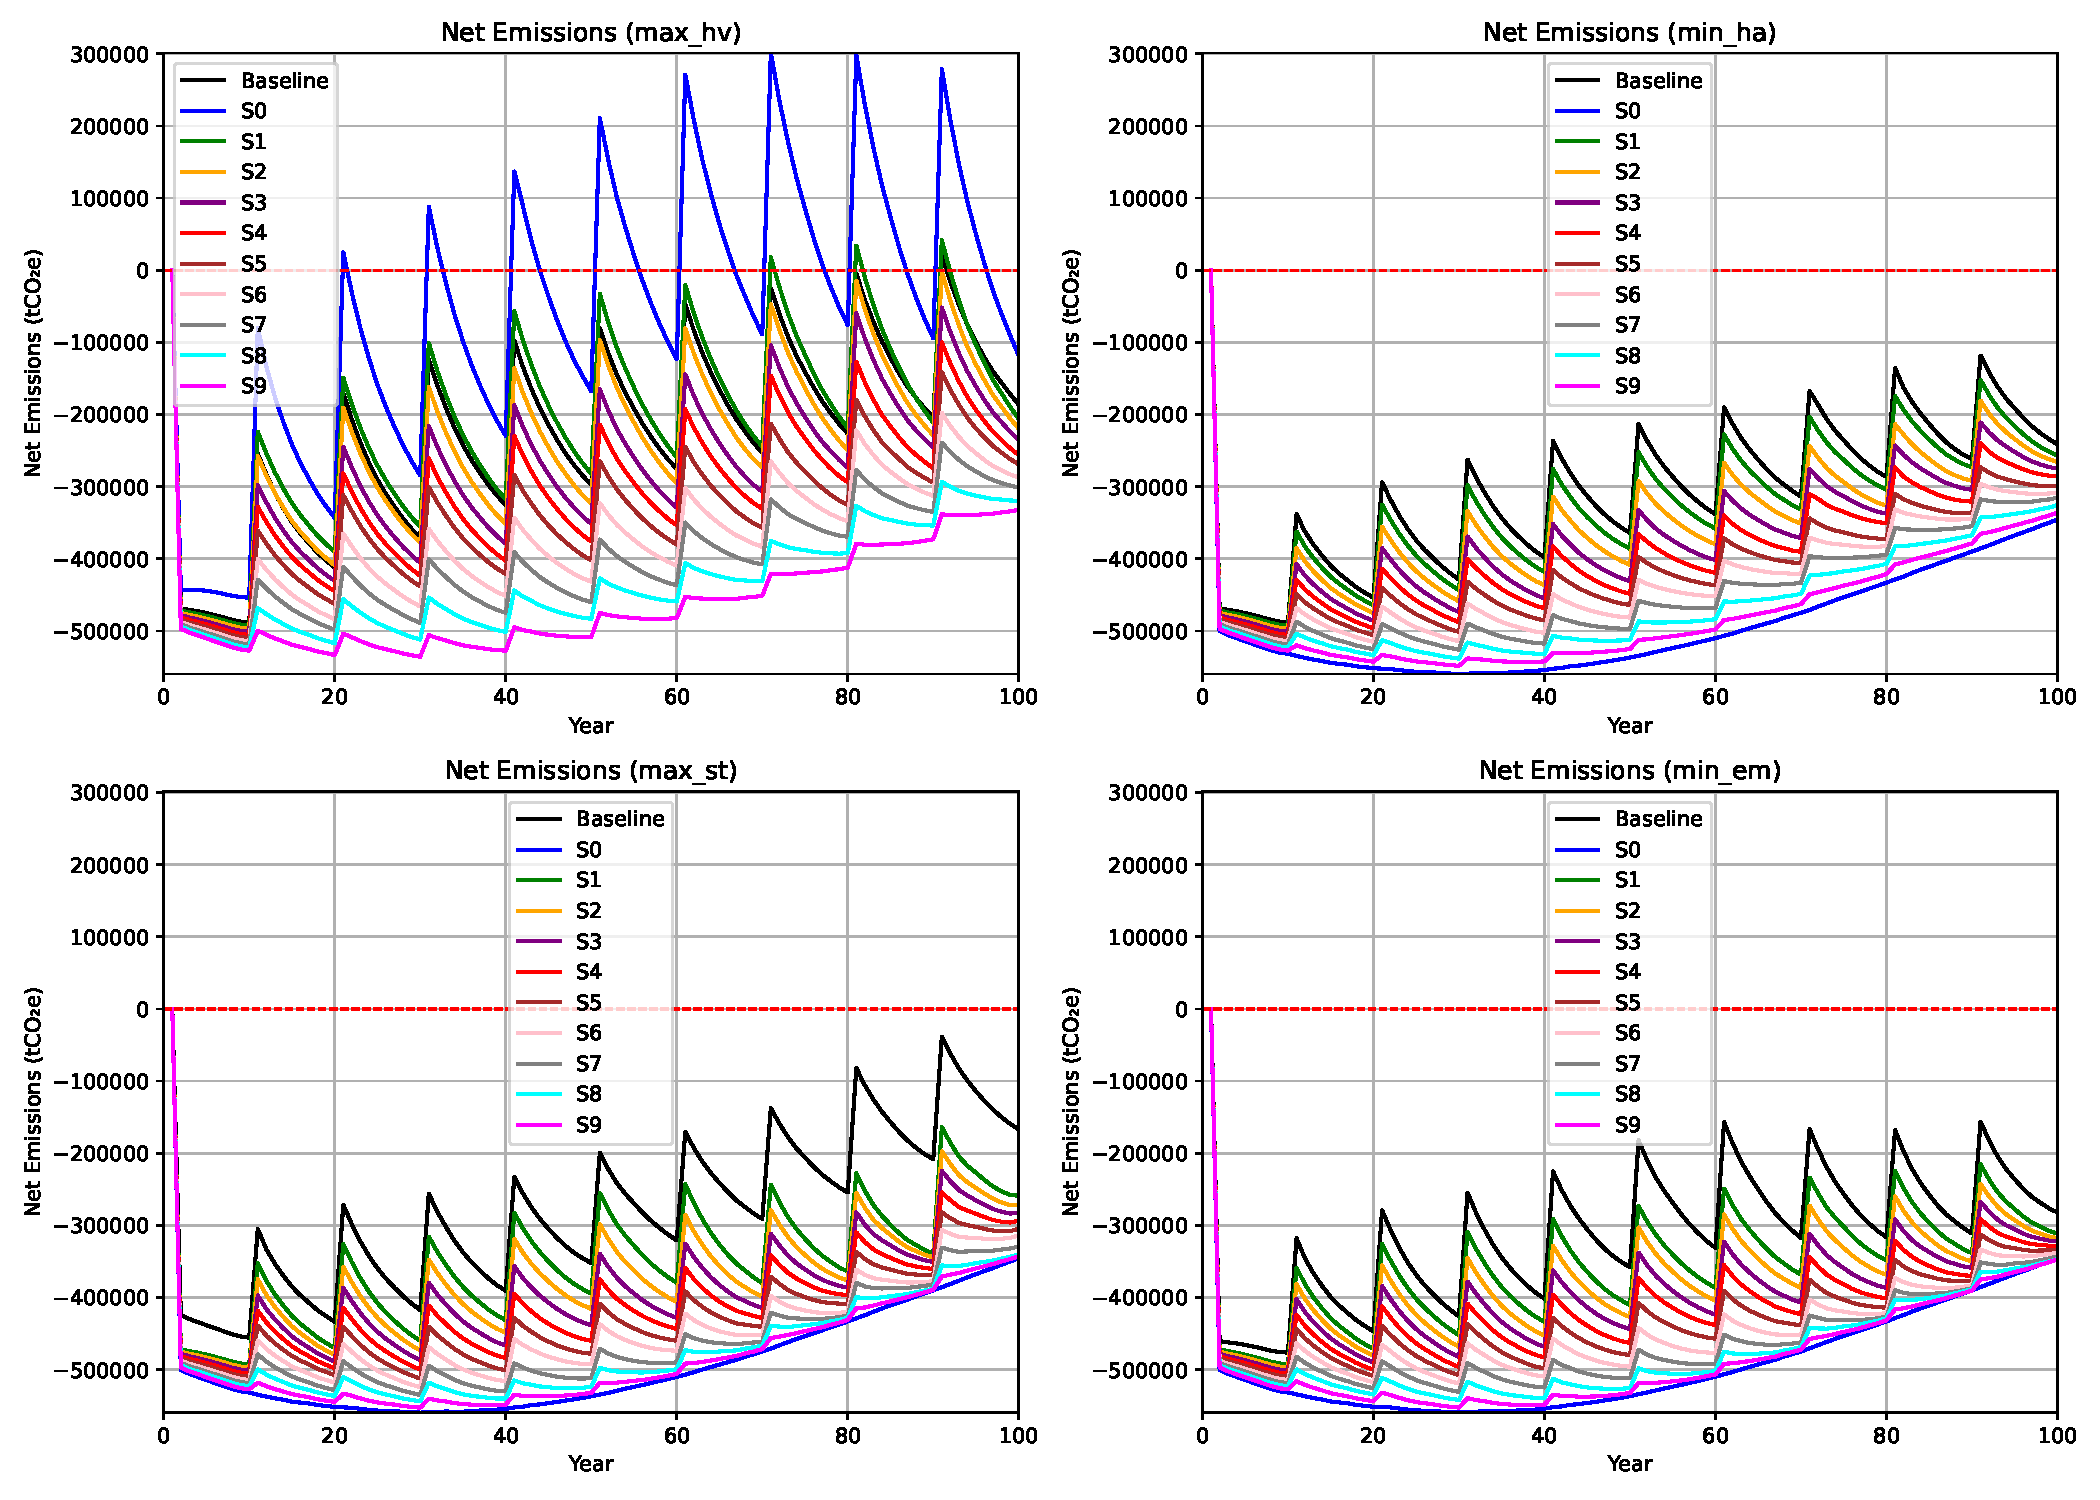
\includegraphics[width=\linewidth]{Fig.A.6.pdf} 
    \caption{Comparison of net emissions across different scenarios and planning objectives in the forest lands surrounding Mining Site 2 over a 100-year planning horizon.}
    \label{fig:Fig.A.6}    
\end{figure}

\begin{figure}[H]
    \centering
    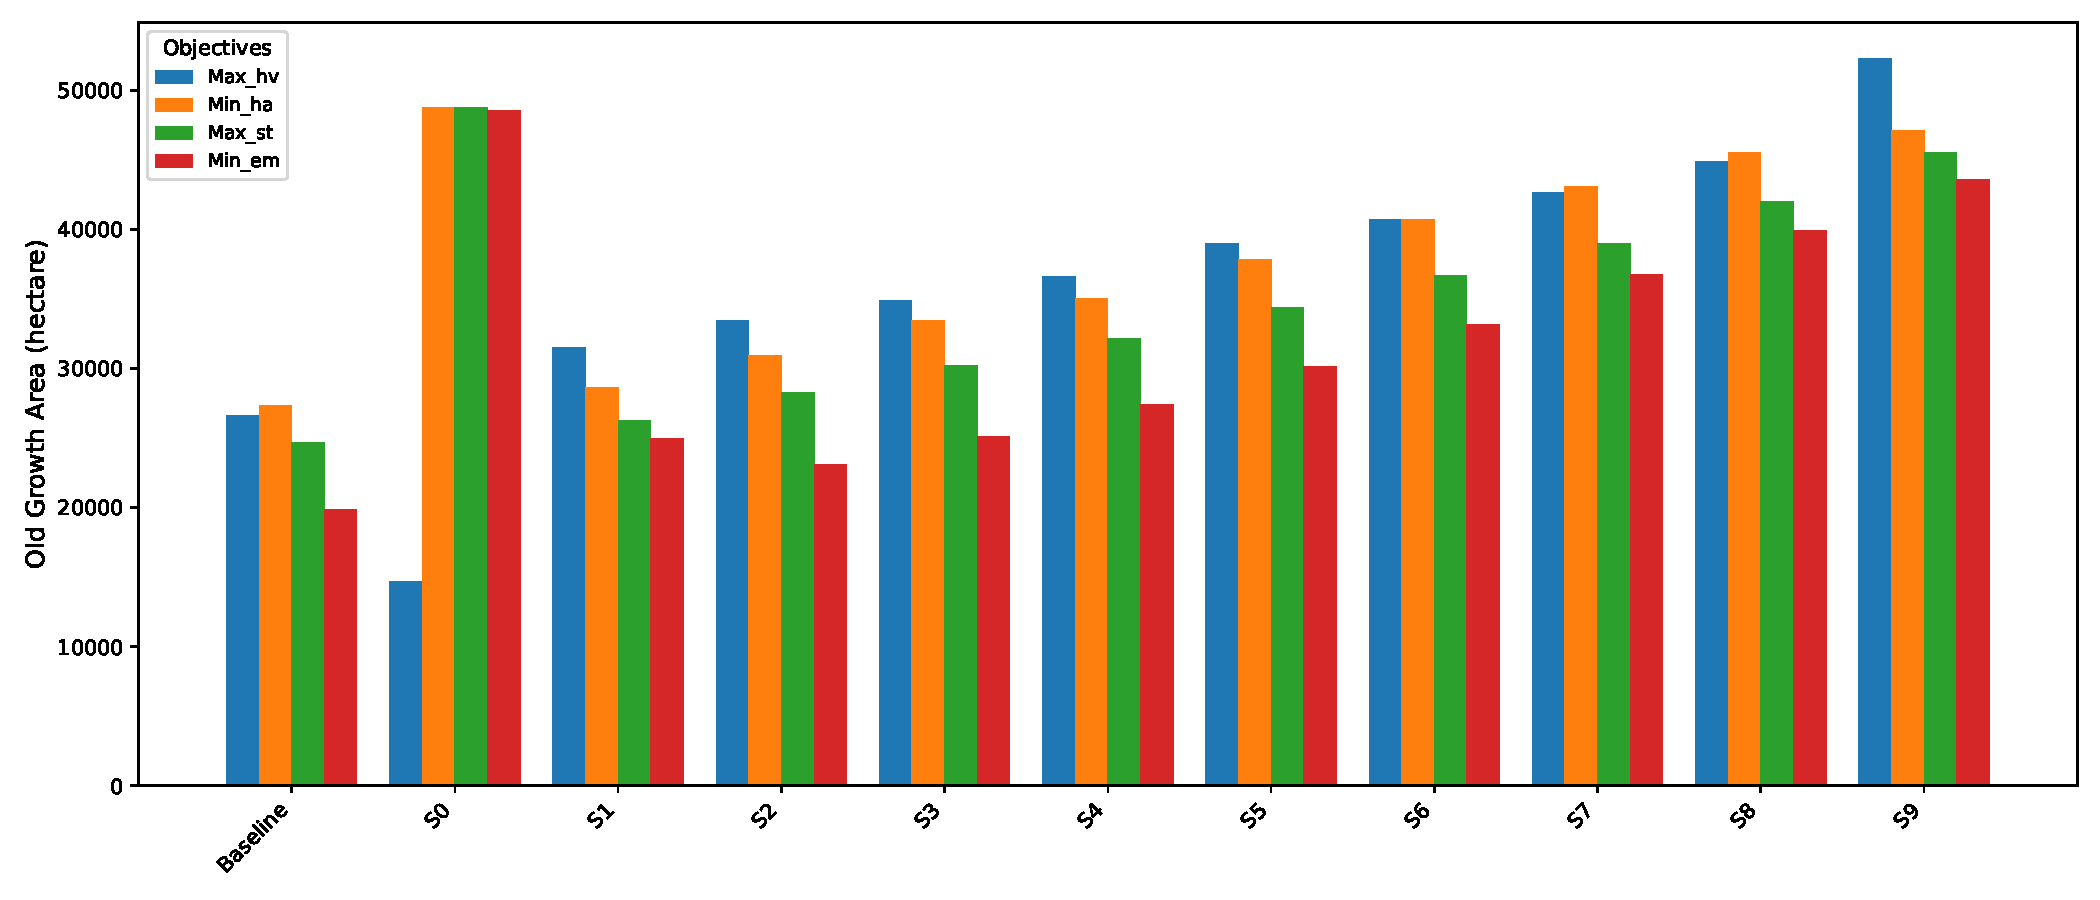
\includegraphics[width=\linewidth]{Fig.A.7.pdf} 
    \caption{Comparison of old growth attributes across harvesting scenarios and planning objectives in the forest lands surrounding Mining Site 2.}
    \label{fig:Fig.A.7}    
\end{figure}

\begin{figure}[H]
    \centering
    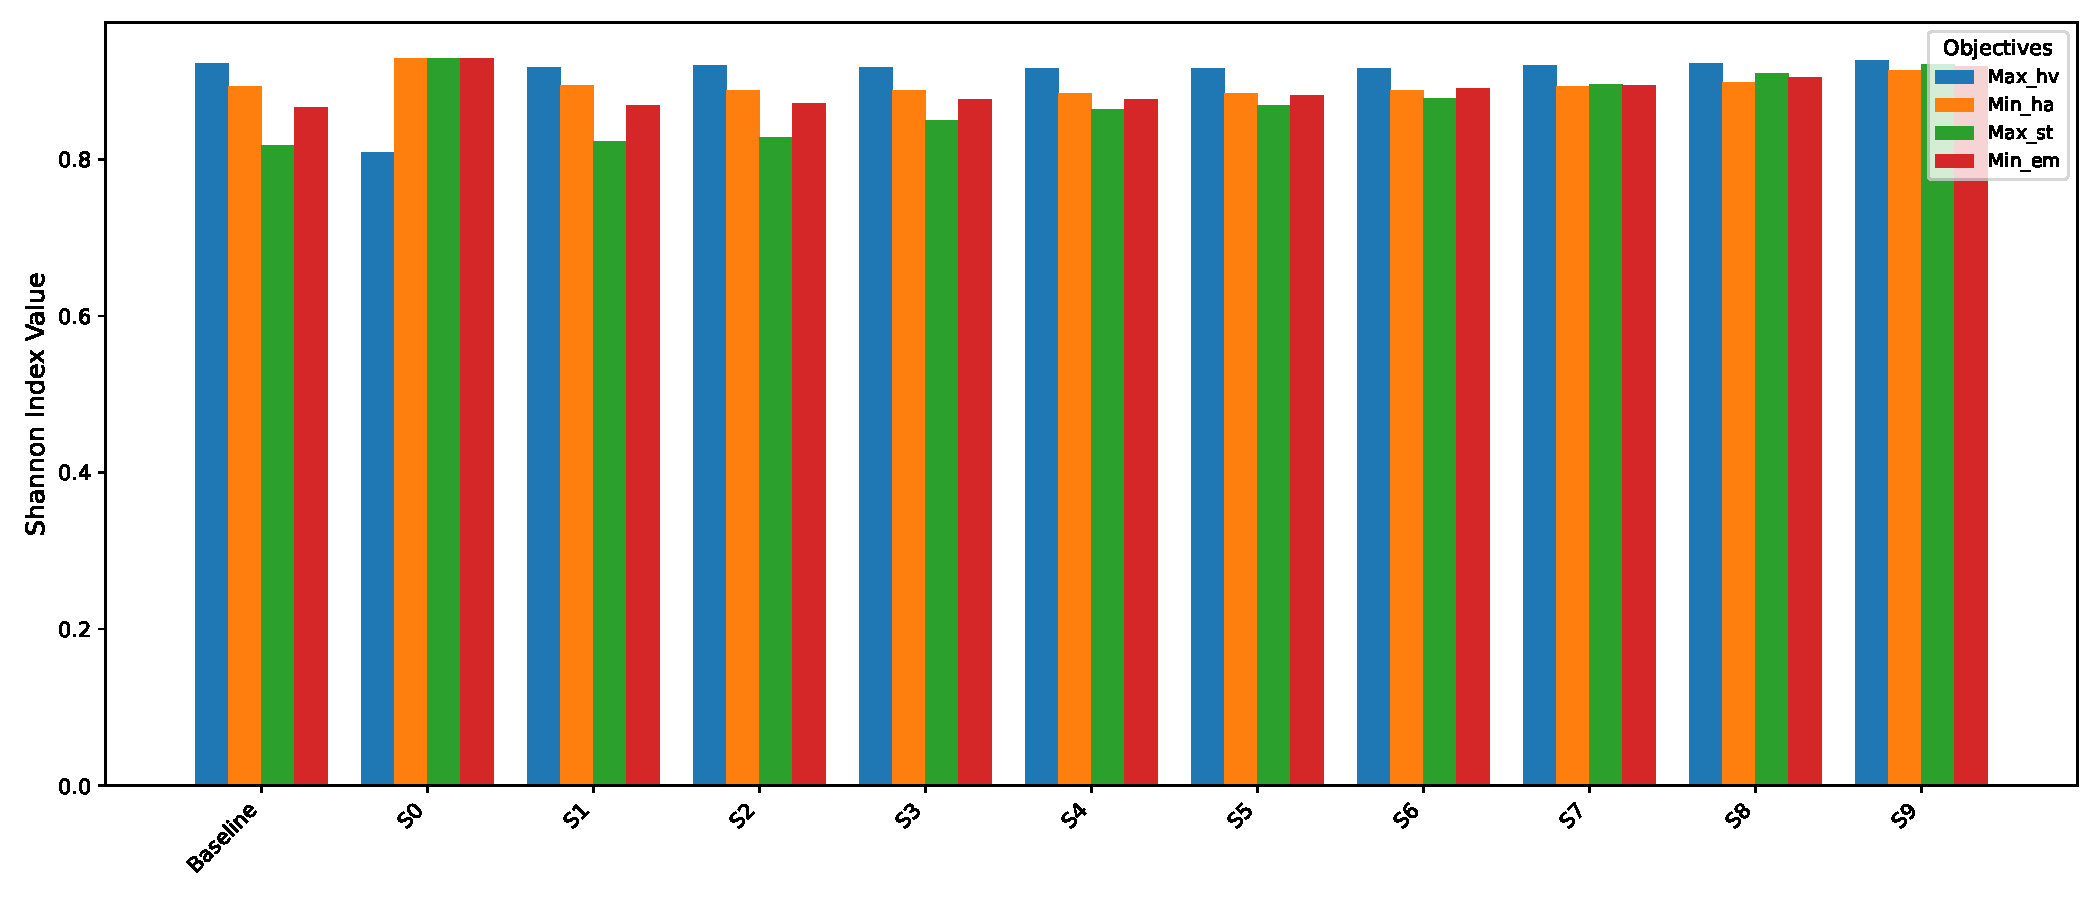
\includegraphics[width=\linewidth]{Fig.A.8.pdf} 
    \caption{Comparison of tree species diversity across harvesting scenarios and planning objectives in the forest lands surrounding Mining Site 2.}
    \label{fig:Fig.A.8}    
\end{figure}

\newpage
\section{Results of Mining Site 3}
\label{sec:appendix3}
\renewcommand{\thetable}{B.\arabic{table}} % Set table numbering in the format A.1, A.2, etc.
\setcounter{table}{0} % Reset the table counter for the appendix section
\setcounter{figure}{0} % Reset the table counter for the appendix section

Here, we present the detailed results from running all defined scenarios under various objectives for Mining Site 3.

\begin{figure}[H]
    \centering
    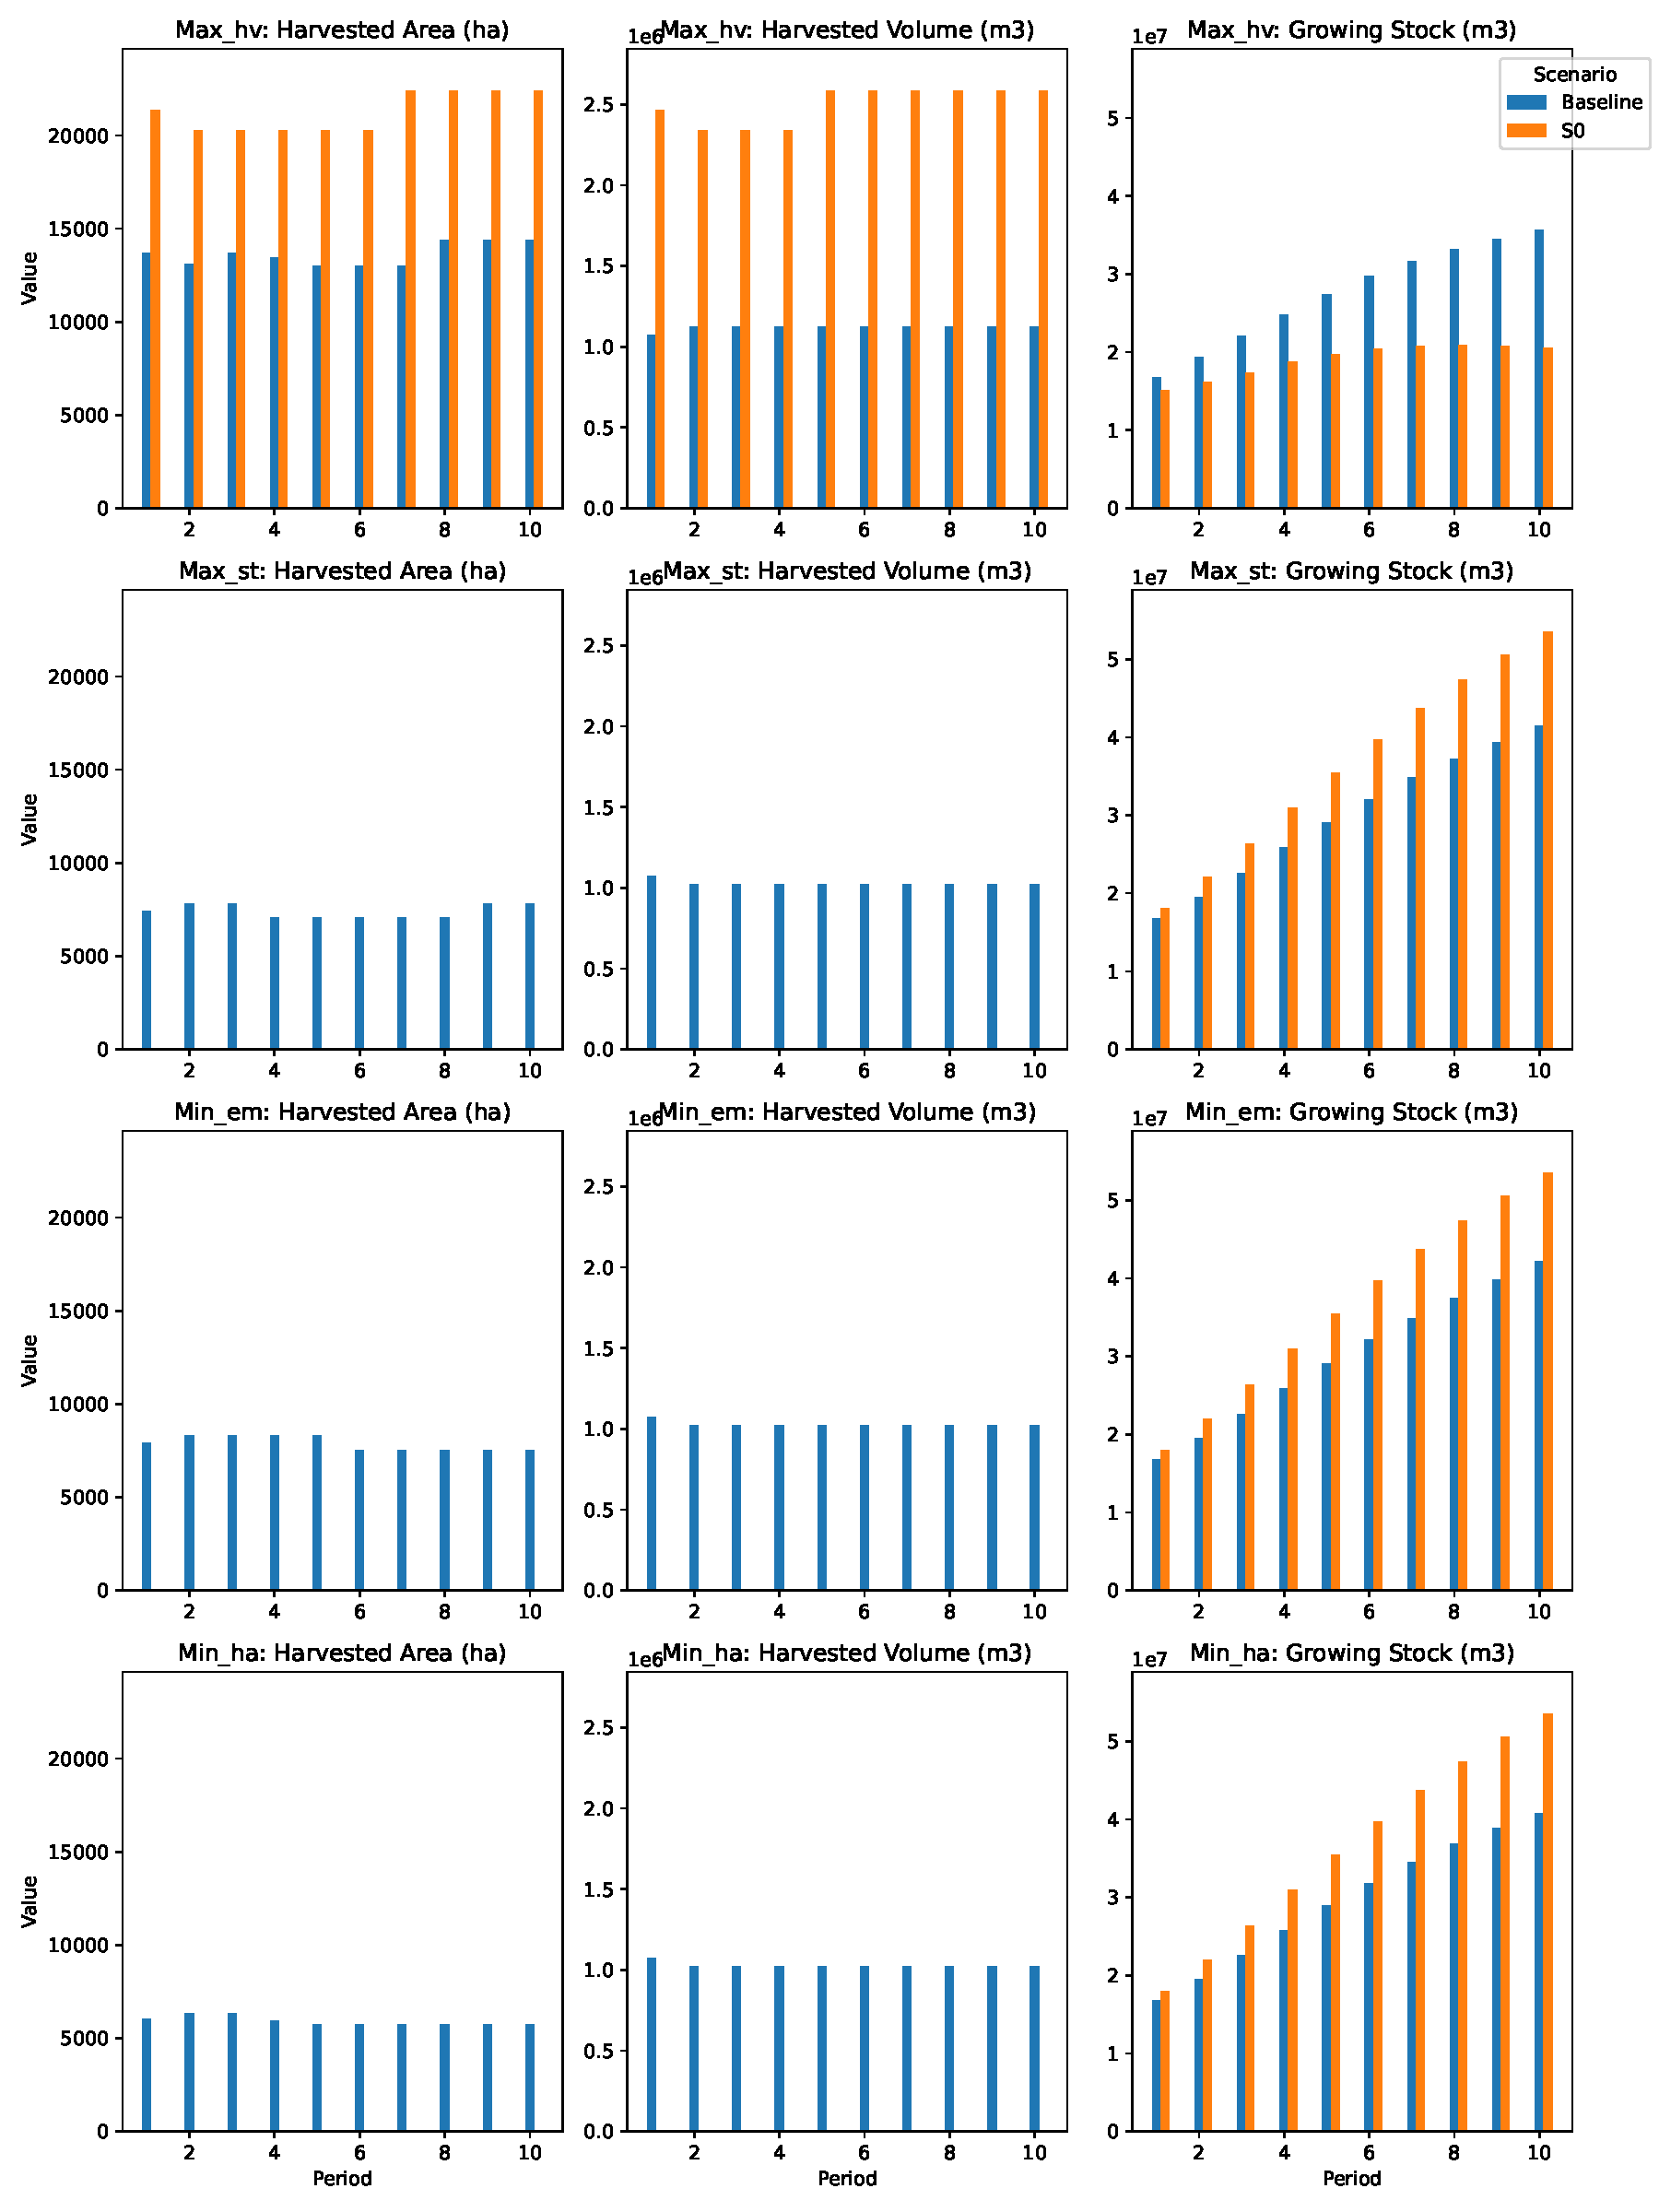
\includegraphics[width=\linewidth]{Fig.B.1.pdf} 
    \caption{Comparison of forest management outcomes in the forest lands surrounding Mining Site 3: Baseline vs. S0 across four objectives.}
    \label{fig:Fig.B.1}    
\end{figure}

\begin{figure}[H]
    \centering
    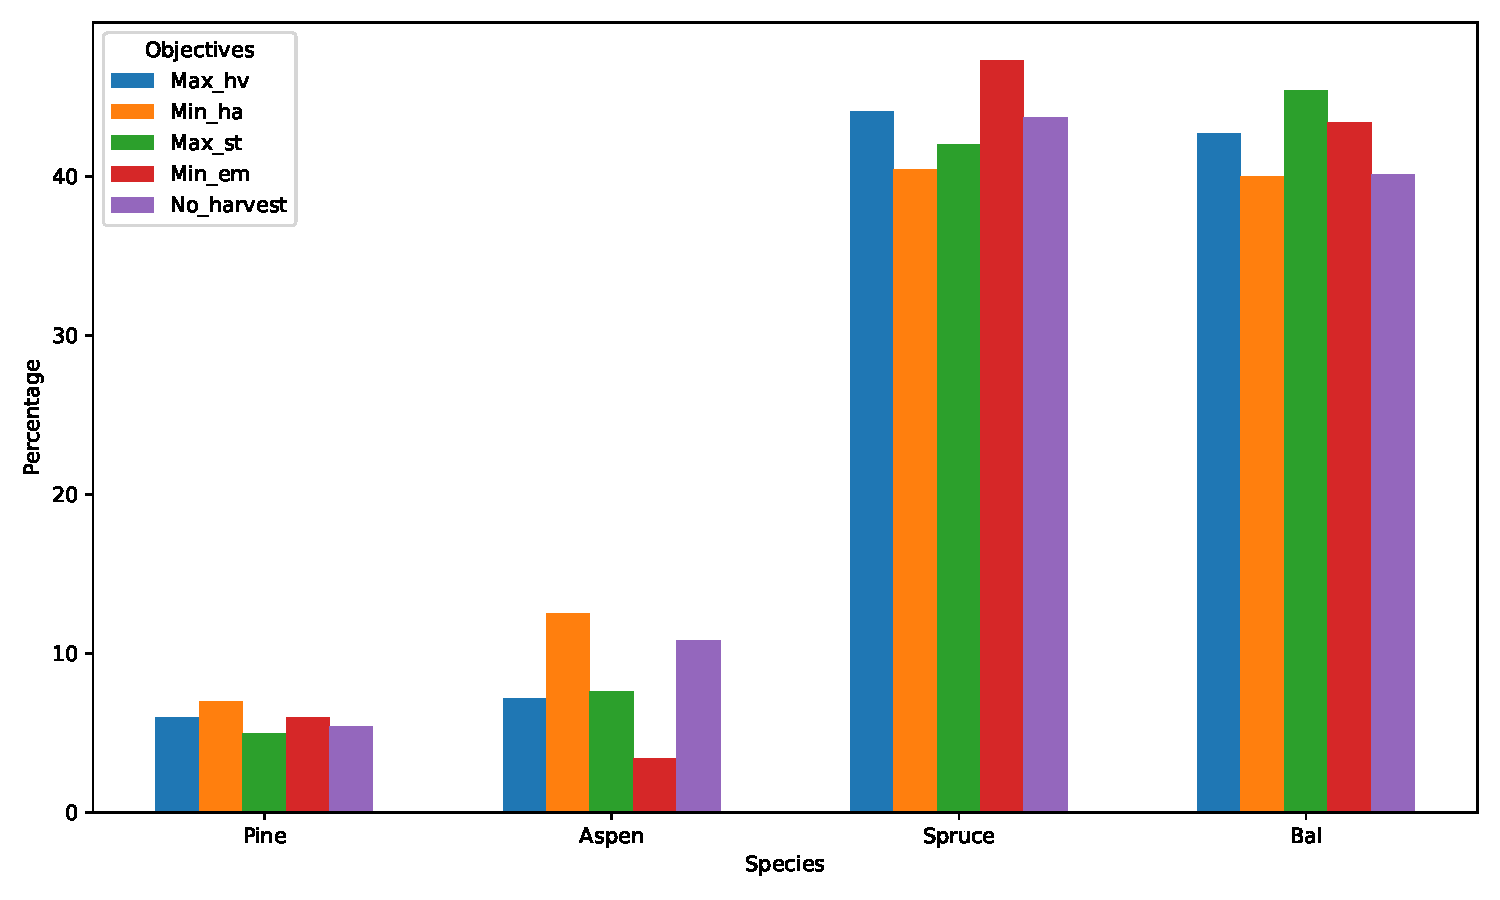
\includegraphics[width=\linewidth]{Fig.B.2.pdf} 
    \caption{Comparison of retained tree species under four management objectives and the no-harvest condition in forest lands surrounding Mining Site 3 (baseline scenario)}
    \label{fig:Fig.B.2}    
\end{figure}

\begin{table}[H]
\centering
\caption{Comparison of KPIs across harvesting scenarios for the forest lands surrounding Mining Site 3 under the objective of maximizing harvested volume.}
\label{tab:KPIs_max_hv_site3}
\begin{adjustbox}{width=\textwidth}
{\small
\begin{tabular}{lrrrr}
\toprule
\makecell[l]{Scenario} & 
\makecell[r]{Harvest\\Volume\\(Mm\textsuperscript{3})} & 
\makecell[r]{Net\\Emissions\\(MtCO\textsubscript{2}e)} & 
\makecell[r]{Species\\Indicator} & 
\makecell[r]{Old Growth\\(k ha)} \\
\midrule
Baseline & 11.21 & -46.08 & 0.780 & 100.4 \\
S0       & 25.00 & -20.55 & 0.730 &  47.2 \\
S1       & 10.09 & -50.23 & 0.777 & 104.5 \\
S2       &  8.97 & -52.65 & 0.783 & 106.8 \\
S3       &  7.85 & -56.56 & 0.785 & 111.0 \\
S4       &  6.73 & -61.57 & 0.779 & 114.1 \\
S5       &  5.61 & -64.19 & 0.771 & 115.2 \\
S6       &  4.48 & -68.33 & 0.773 & 119.9 \\
S7       &  3.36 & -71.72 & 0.781 & 124.7 \\
S8       &  2.24 & -76.11 & 0.780 & 128.3 \\
S9       &  1.12 & -78.93 & 0.799 & 139.2 \\
\bottomrule
\end{tabular}
}
\end{adjustbox}
\end{table}

\begin{table}[H]
\centering
\caption{Comparison of KPIs across harvesting scenarios for the forest lands surrounding Mining Site 3 under the objective of maximizing carbon stock.}
\label{tab:KPIs_max_cs_site3}
\begin{adjustbox}{width=\textwidth}
{\small
\begin{tabular}{lrrrrr}
\toprule
\makecell[l]{Scenario} & 
\makecell[r]{Harvest\\Volume\\($\mathrm{Mm}^3$)} &
\makecell[r]{Carbon\\Stock\\(MtC)} & 
\makecell[r]{Net\\Emissions\\(MtCO\textsubscript{2}e)} & 
\makecell[r]{Species\\Indicator} & 
\makecell[r]{Old Growth\\(k ha)} \\
\midrule
Baseline & 10.25 & 69.02 & -61.35 & 0.770 & 101.9 \\
S0       & -     & 72.96 & -81.55 & 0.812 & 150.2 \\
S1       & 9.22  & 69.49 & -63.71 & 0.776 & 107.0 \\
S2       & 8.20  & 69.95 & -66.06 & 0.782 & 112.3 \\
S3       & 7.17  & 70.41 & -68.41 & 0.784 & 117.1 \\
S4       & 6.15  & 70.85 & -70.66 & 0.785 & 121.9 \\
S5       & 5.12  & 71.29 & -72.75 & 0.785 & 126.7 \\
S6       & 4.10  & 71.71 & -74.81 & 0.789 & 132.1 \\
S7       & 3.07  & 72.11 & -76.81 & 0.792 & 137.5 \\
S8       & 2.05  & 72.48 & -78.79 & 0.793 & 141.7 \\
S9       & 1.02  & 72.78 & -80.47 & 0.804 & 146.2 \\
\bottomrule
\end{tabular}
}
\end{adjustbox}
\end{table}


\begin{table}[H]
\centering
\caption{Comparison of KPIs across harvesting scenarios for the forest lands surrounding Mining Site 3 under the objective of minimizing net emissions.}
\label{tab:KPIs_min_em_site3}
\begin{adjustbox}{width=\textwidth}
{\small
\begin{tabular}{lrrrrr}
\toprule
\makecell[l]{Scenario} & 
\makecell[r]{Harvest\\Volume\\($\mathrm{Mm}^3$)} &
\makecell[r]{Net\\Emissions\\(MtCO\textsubscript{2}e)} & 
\makecell[r]{Species\\Indicator} & 
\makecell[r]{Old Growth\\(k ha)} \\
\midrule
Baseline & 10.25 & -62.35 & 0.721 & 76.6 \\
S0       & 0.04 & -81.52 & 0.812 & 150.0 \\
S1       & 9.22 & -64.60 & 0.743 & 85.2 \\
S2       & 8.20 & -66.80 & 0.751 & 92.8 \\
S3       & 7.17 & -68.91 & 0.754 & 99.5 \\
S4       & 6.15 & -70.96 & 0.754 & 104.1 \\
S5       & 5.12 & -72.96 & 0.751 & 111.3 \\
S6       & 4.10 & -75.04 & 0.769 & 121.1 \\
S7       & 3.07 & -77.01 & 0.783 & 130.6 \\
S8       & 2.05 & -78.90 & 0.792 & 138.7 \\
S9       & 1.02 & -80.49 & 0.801 & 145.0 \\
\bottomrule
\end{tabular}
}
\end{adjustbox}
\end{table}

\begin{table}[H]
\centering
\caption{Comparison of KPIs across harvesting scenarios for the forest lands surrounding Mining Site 3 under the objective of minimizing harvested area.}
\label{tab:KPIs_min_ha_site3}
\begin{adjustbox}{width=\textwidth}
{\small
\begin{tabular}{lrrrrr}
\toprule
\makecell[l]{Scenario} & 
\makecell[r]{Harvest\\Volume\\($\mathrm{Mm}^3$)} &
\makecell[r]{Harvest\\Area\\(k ha)} & 
\makecell[r]{Net\\Emissions\\(MtCO\textsubscript{2}e)} & 
\makecell[r]{Species\\Indicator} & 
\makecell[r]{Old Growth\\(k ha)} \\
\midrule
Baseline & 10.25 & 59.13  & -60.13 & 0.851 & 111.3 \\
S0       & -    & --     & -81.55 & 0.812 & 150.2 \\
S1       & 9.22 & 52.32  & -62.49 & 0.846 & 116.2 \\
S2       & 8.20 & 45.73  & -64.83 & 0.844 & 119.1 \\
S3       & 7.17 & 39.33  & -67.15 & 0.837 & 122.5 \\
S4       & 6.15 & 33.09  & -69.38 & 0.834 & 126.5 \\
S5       & 5.12 & 27.02  & -71.59 & 0.828 & 129.8 \\
S6       & 4.10 & 21.15  & -73.78 & 0.823 & 133.7 \\
S7       & 3.07 & 15.50  & -75.96 & 0.818 & 138.6 \\
S8       & 2.05 & 10.02  & -77.71 & 0.818 & 142.0 \\
S9       & 1.02 & 4.76   & -79.63 & 0.816 & 146.7 \\
\bottomrule
\end{tabular}
}
\end{adjustbox}
\end{table}


\begin{figure}[H]
    \centering
    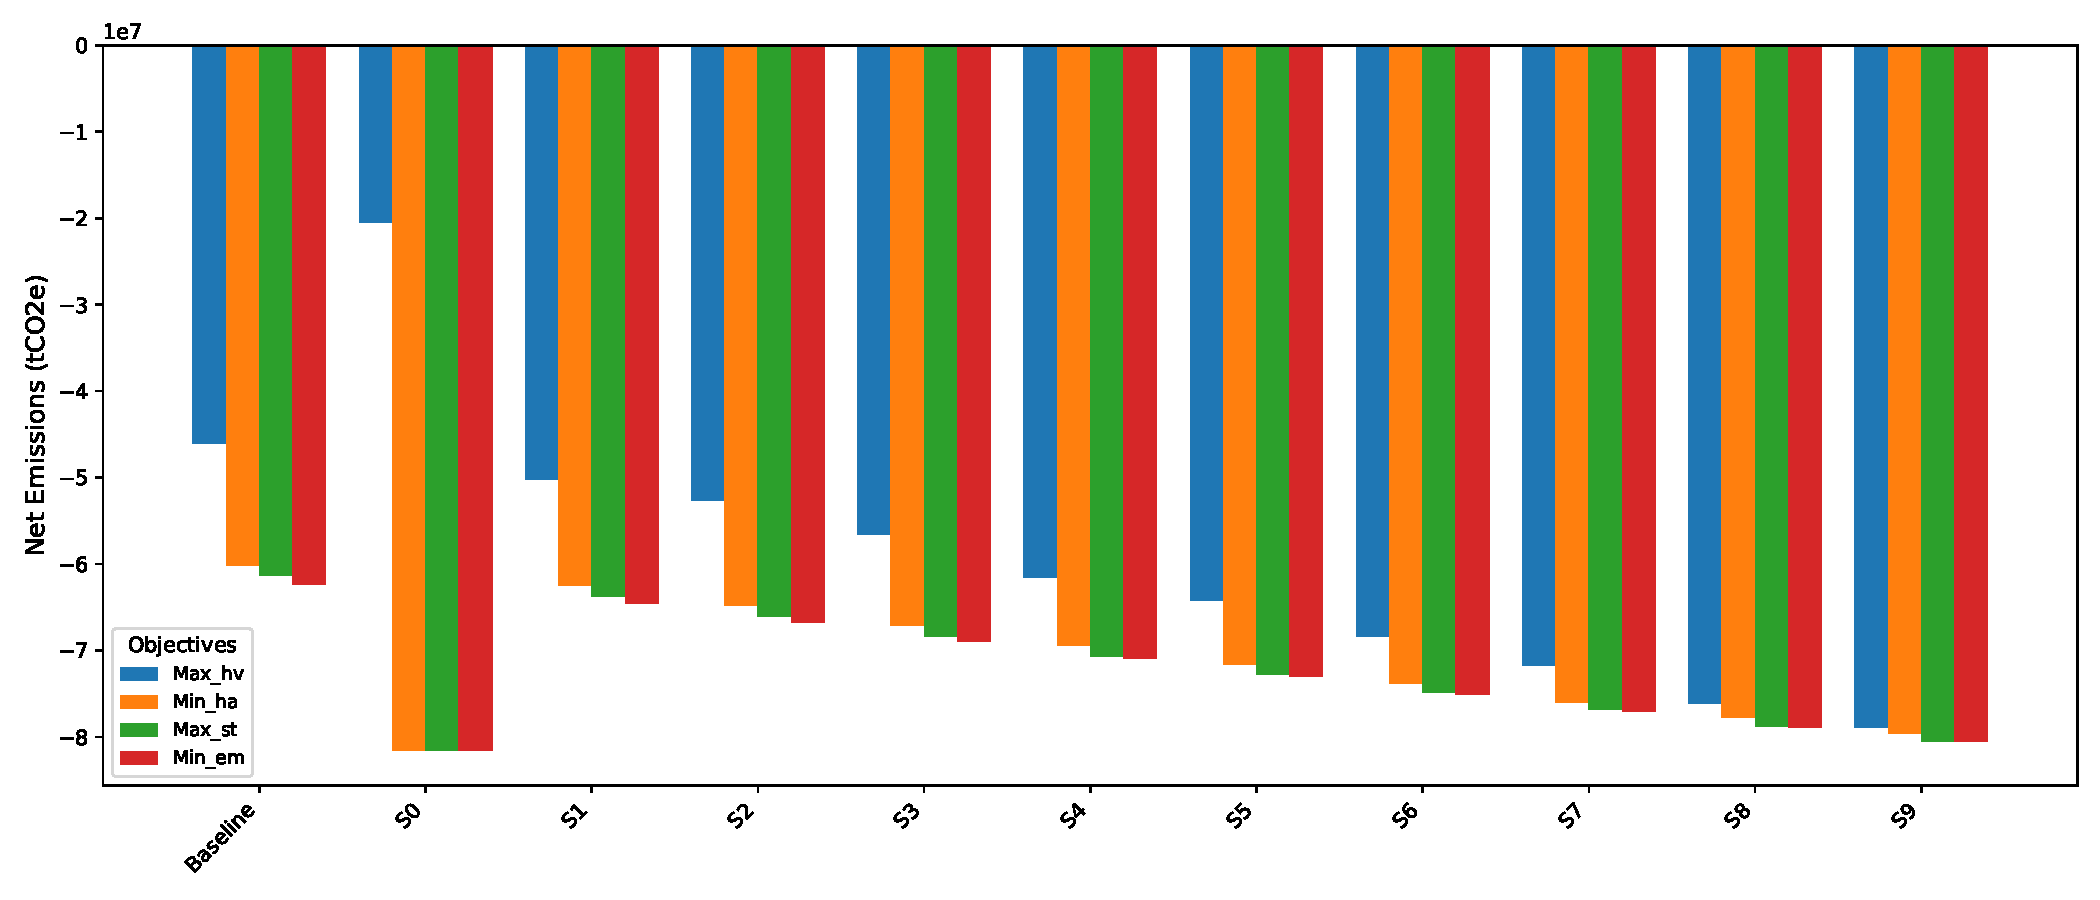
\includegraphics[width=\linewidth]{Fig.B.5.pdf} 
    \caption{Comparison of net emissions across different scenarios and planning objectives in the forest lands surrounding Mining site 3.}
    \label{fig:Fig.B.5}    
\end{figure}

\begin{figure}[H]
    \centering
    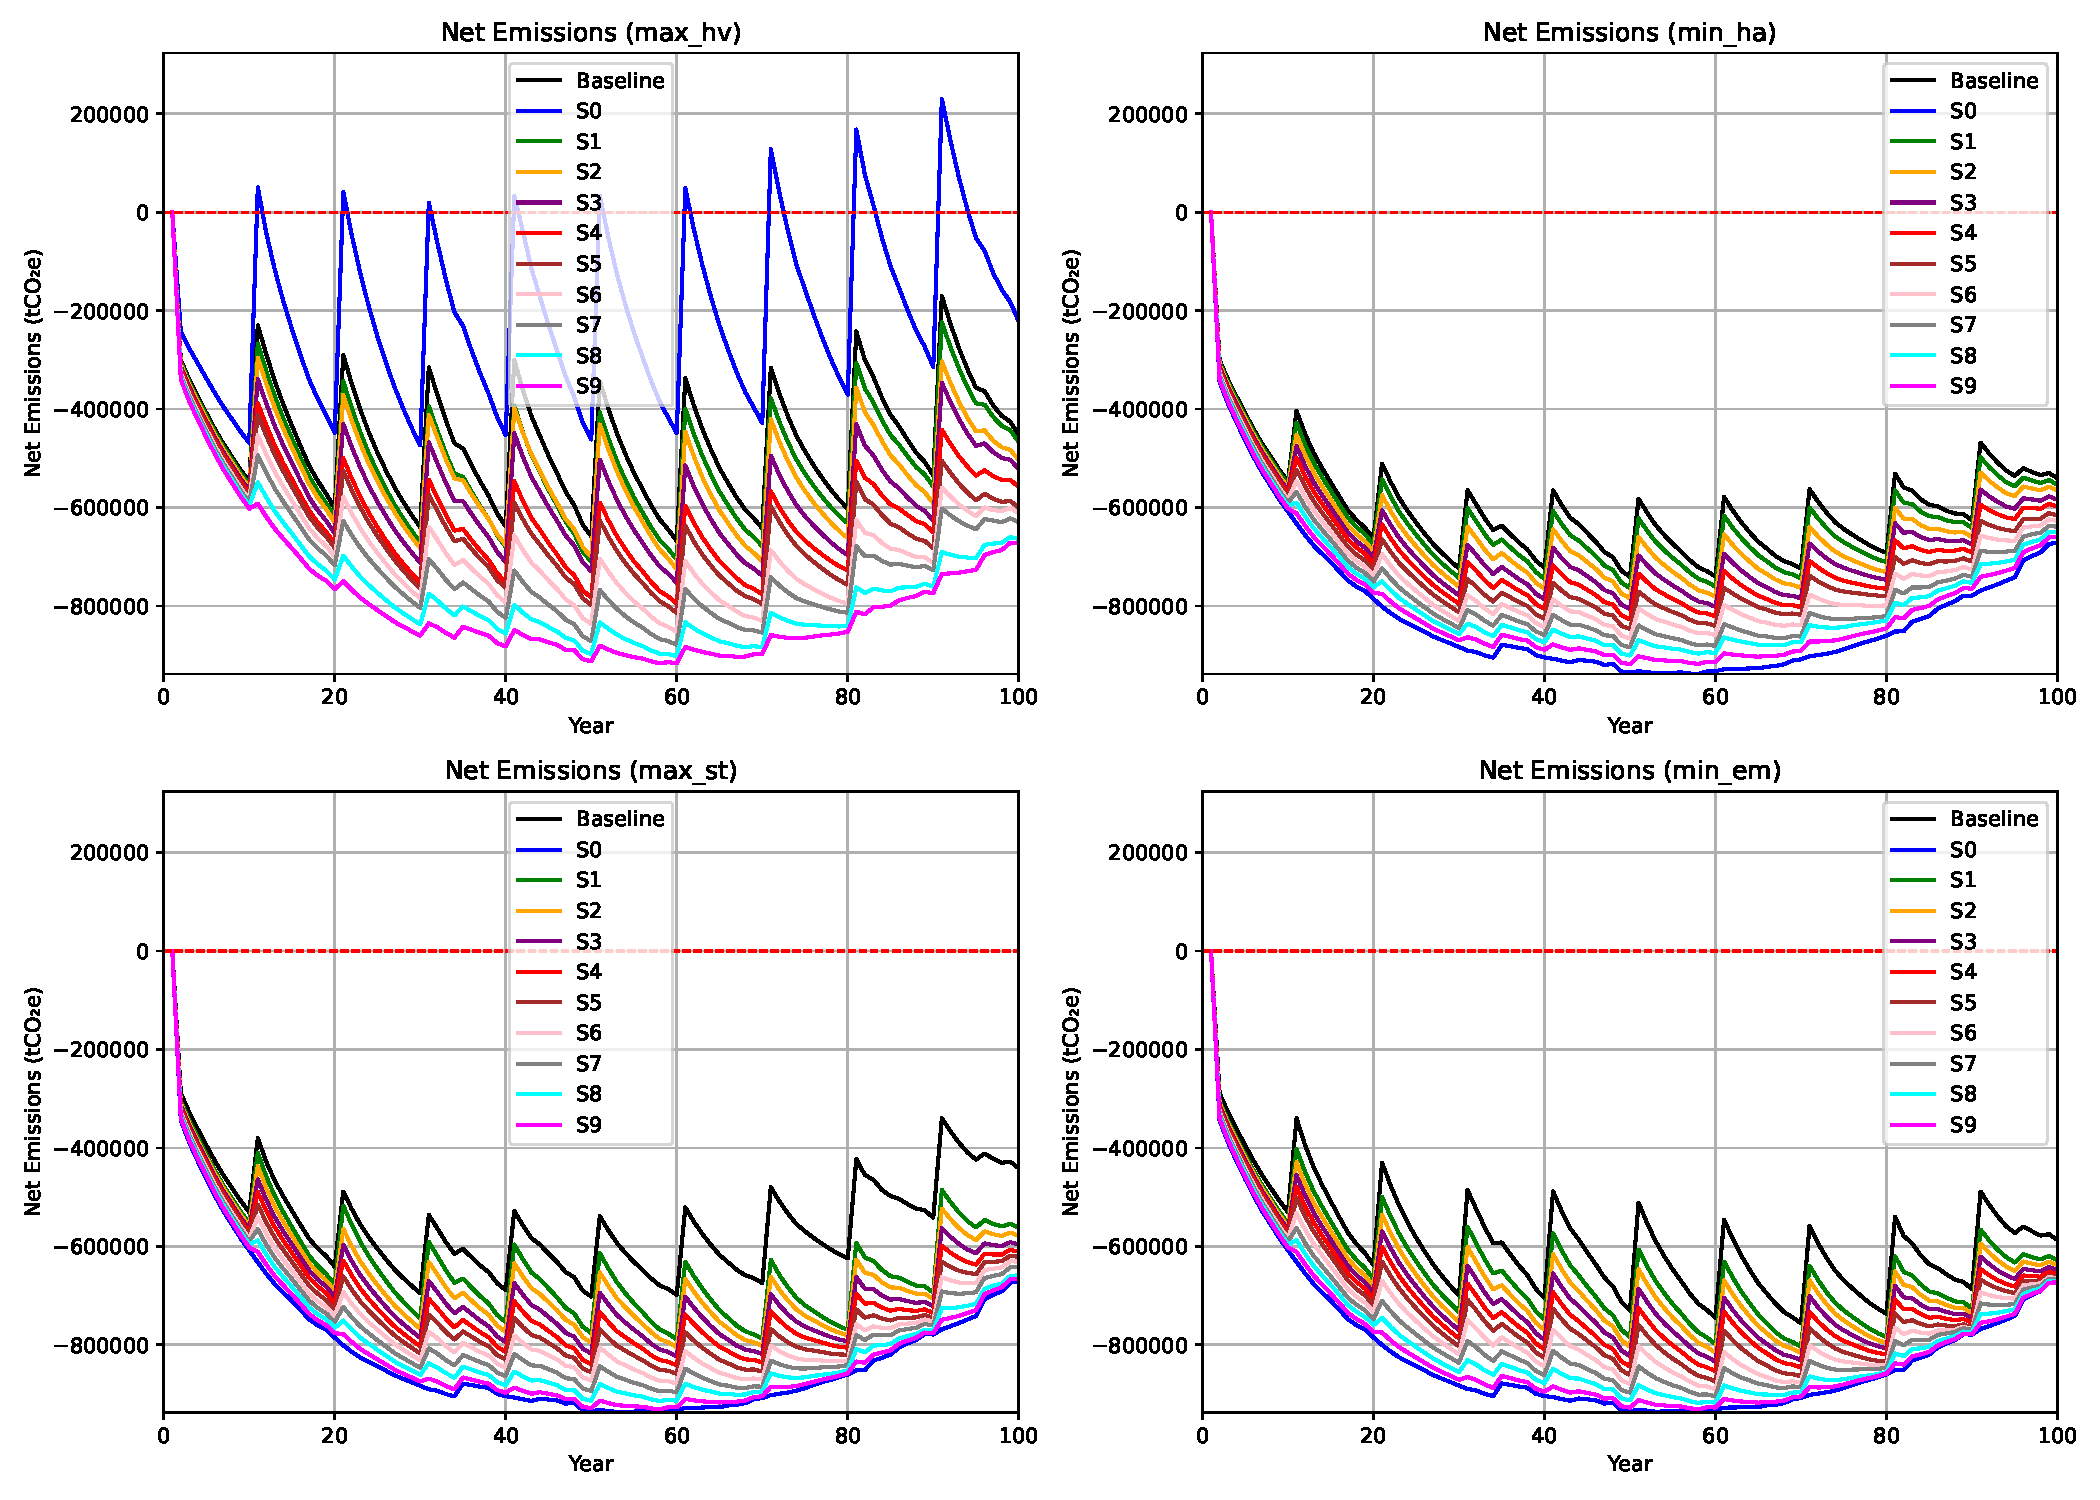
\includegraphics[width=\linewidth]{Fig.B.6.pdf} 
    \caption{Comparison of net emissions across different scenarios and planning objectives in the forest lands surrounding Mining Site 3 over a 100-year planning horizon.}
    \label{fig:Fig.B.6}    
\end{figure}

\begin{figure}[H]
    \centering
    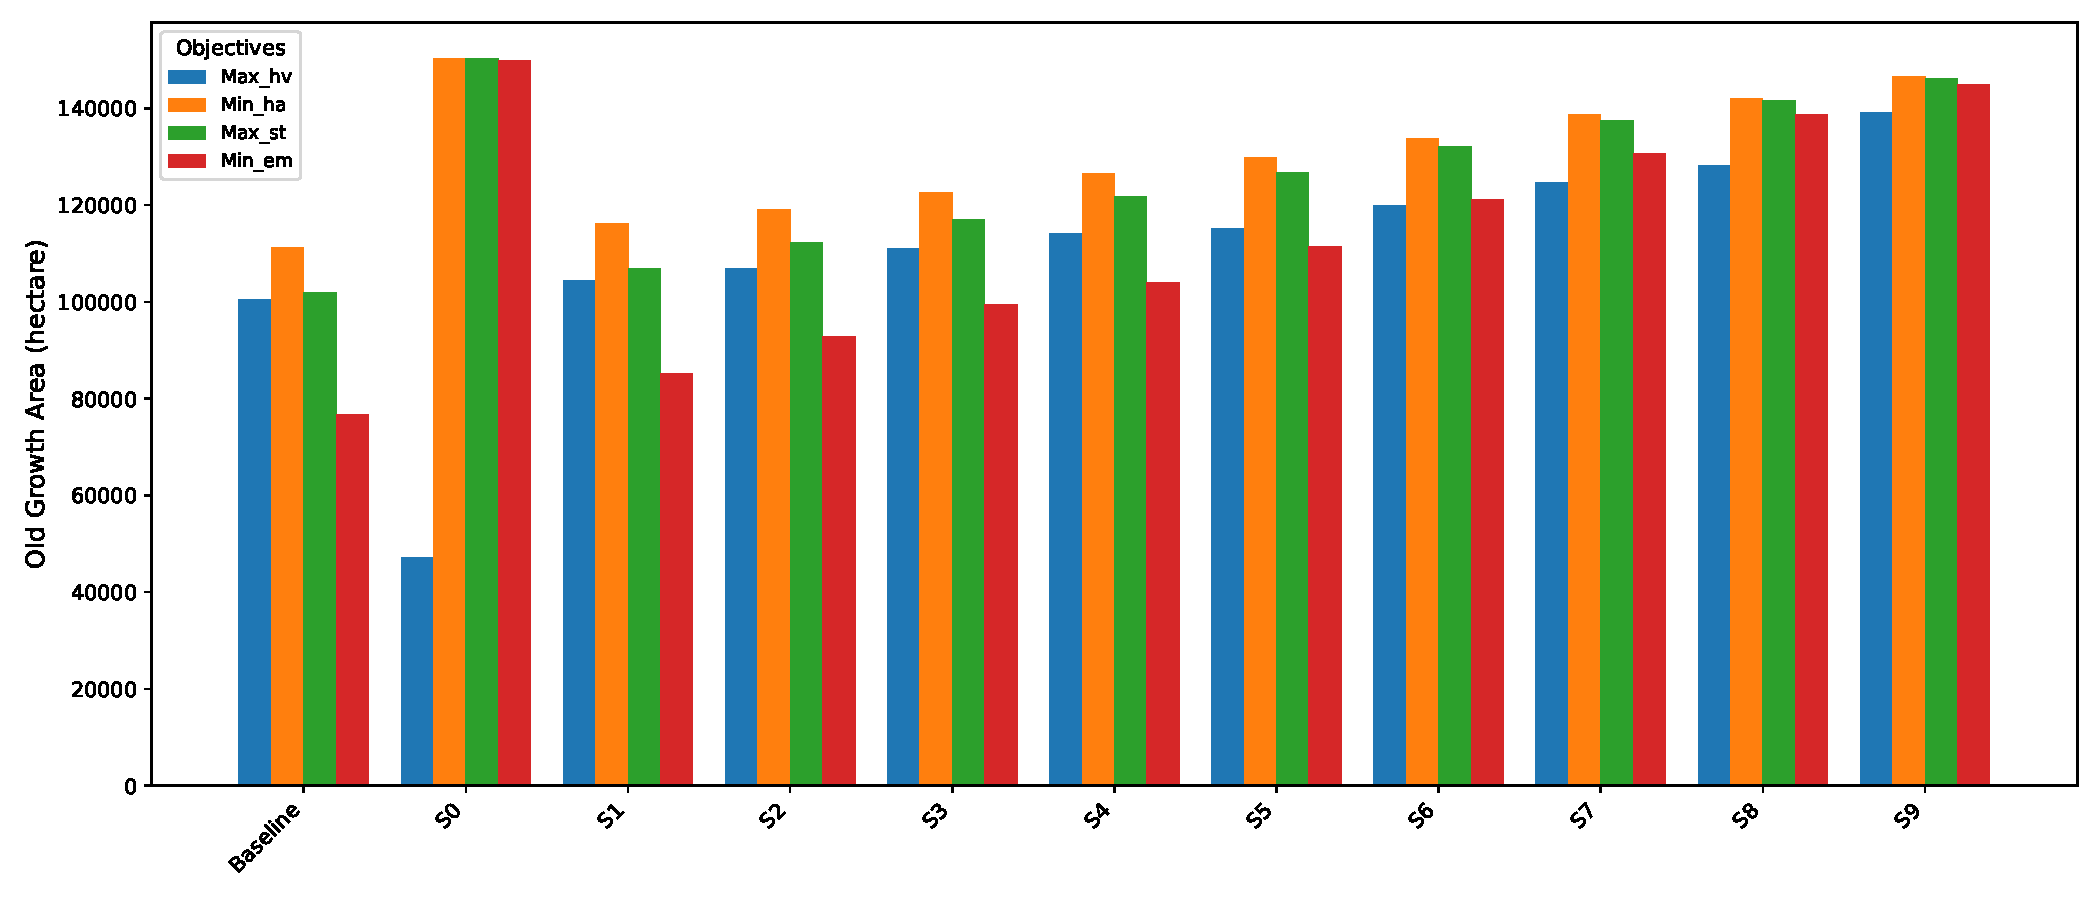
\includegraphics[width=\linewidth]{Fig.B.7.pdf} 
    \caption{Comparison of old growth attributes across harvesting scenarios and planning objectives in the forest lands surrounding Mining Site 3.}
    \label{fig:Fig.B.7}    
\end{figure}

\begin{figure}[H]
    \centering
    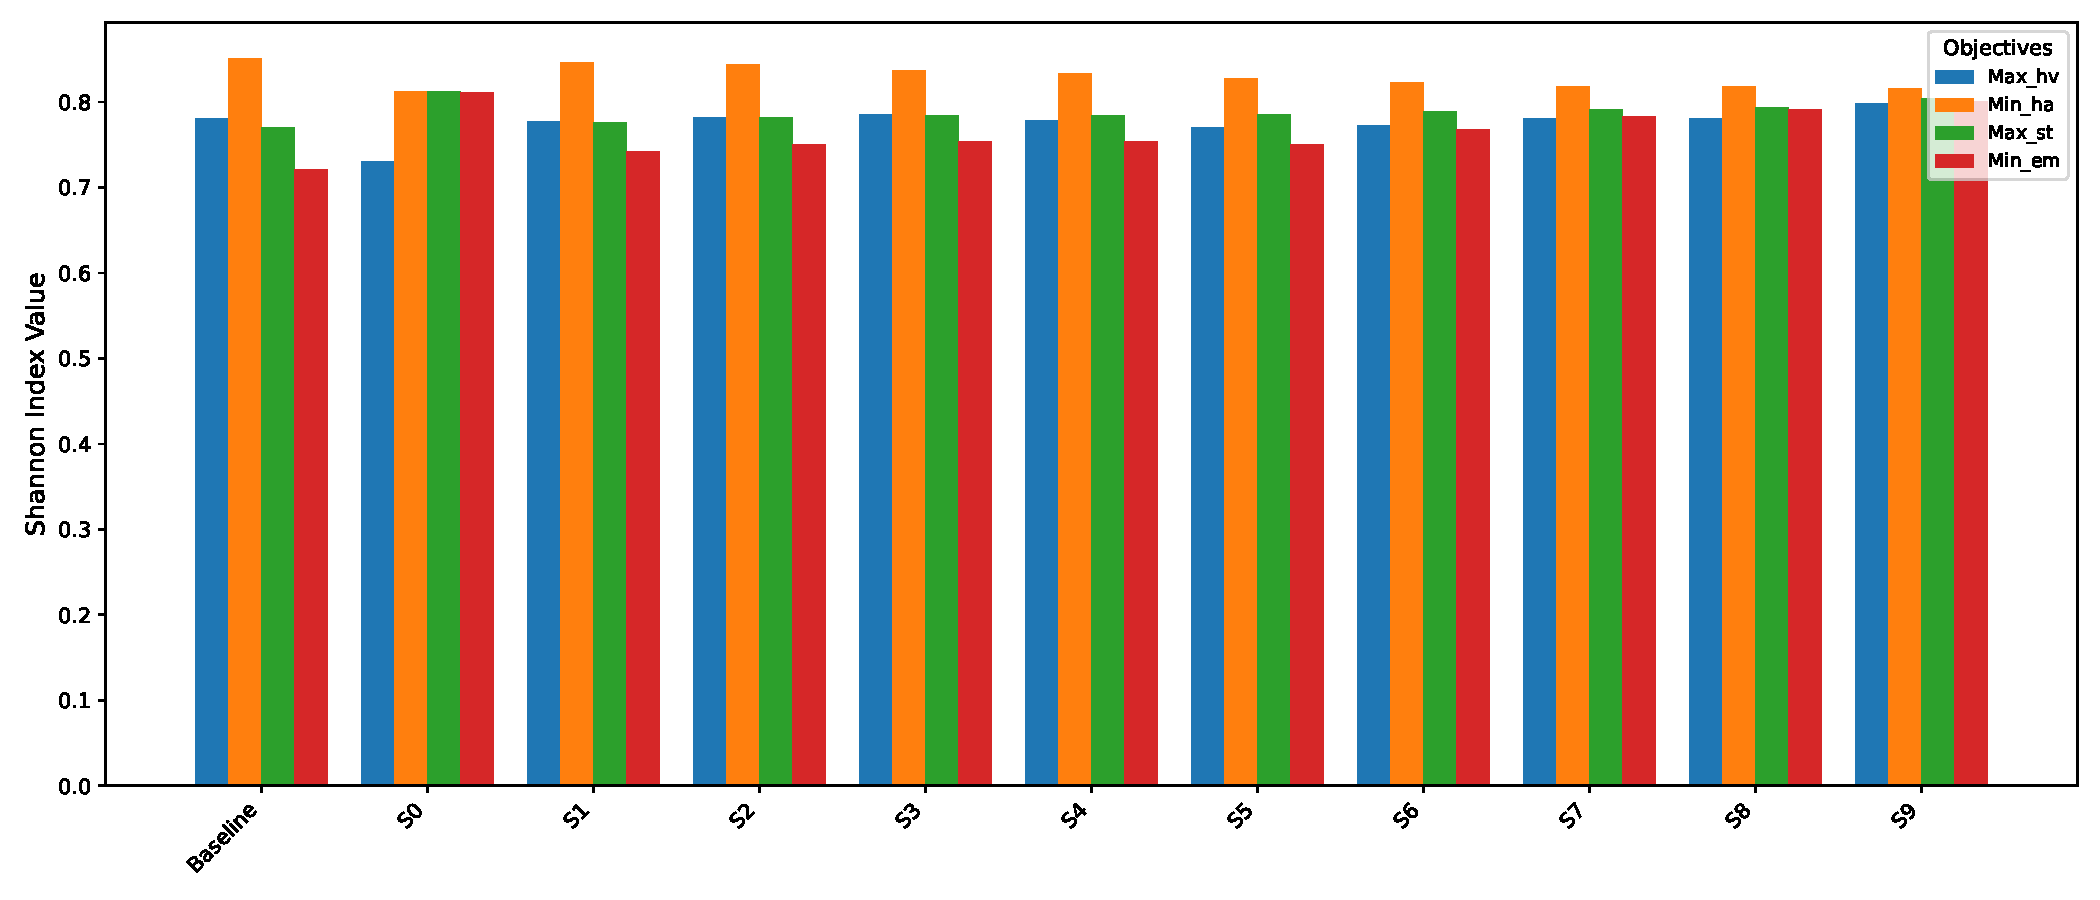
\includegraphics[width=\linewidth]{Fig.B.8.pdf} 
    \caption{Comparison of tree species diversity across harvesting scenarios and planning objectives in the forest lands surrounding Mining Site 3.}
    \label{fig:Fig.B.8}    
\end{figure}

\end{document}
\endinput